\documentclass[12pt,a4paper,openany]{book}

% Librerias

\usepackage{babel}
\babelprovide[main,import]{spanish}
\usepackage[utf8]{inputenc}
\usepackage[T1]{fontenc}
\usepackage[sfdefault,scale=0.96]{plex-sans}
\usepackage[scale=0.91]{plex-mono}

% Permite a pdfTeX realizar ajustes tipográficos mínimos en el cuerpo del texto.
% Otros motores, como XeTeX, no exponen estas primitivas.
\AtBeginDocument{%
	\ifdefined\pdffontexpand
		\pdffontexpand\font 25 25 1 autoexpand
		\pdfadjustspacing=2
	\fi
}

\usepackage{amsmath, amssymb}
\usepackage{siunitx}
\sisetup{
	output-decimal-marker = {,},
	inter-unit-product = \cdot,
	exponent-product = \cdot,
	per-mode = symbol
}

\usepackage{tabularx}
\usepackage{booktabs}
\setlength{\extrarowheight}{2pt}
\renewcommand{\arraystretch}{1.18}
\newcolumntype{Y}{>{\raggedright\arraybackslash}X}
\newcolumntype{Z}{>{\centering\arraybackslash}X}
\newcolumntype{L}[1]{>{\raggedright\arraybackslash}p{#1}}
\newcolumntype{C}[1]{>{\centering\arraybackslash}p{#1}}
\usepackage{float}

\usepackage{graphicx}
\usepackage{caption}
\captionsetup[figure]{justification=centering, singlelinecheck=false}
\captionsetup[table]{justification=centering, singlelinecheck=false}
\renewcommand{\tablename}{Tabla}
\addto\captionsspanish{\renewcommand{\tablename}{Tabla}}

\usepackage[top=2.5cm, bottom=2.5cm, left=1.5cm, right=1.5cm]{geometry}
\raggedbottom
\setlength{\emergencystretch}{0.5em}
\tolerance=1800
\setlength{\parskip}{0.55em}

\usepackage{xcolor}
\definecolor{codeback}{RGB}{252,251,255}
\definecolor{coderule}{RGB}{218,212,232}
\definecolor{codeviolet}{RGB}{109,78,180}
\definecolor{codeblue}{RGB}{48,97,171}
\definecolor{codestring}{RGB}{38,127,118}
\definecolor{codecomment}{RGB}{118,124,132}
\definecolor{codenumber}{RGB}{142,134,164}
\definecolor{technicalviolet}{RGB}{98,64,150}
\definecolor{placeholdergray}{RGB}{248,248,248}
\definecolor{placeholderline}{RGB}{160,160,160}

\DeclareTextFontCommand{\texttt}{\ttfamily\color{technicalviolet}}
\newcommand{\tech}[1]{\mbox{\texttt{#1}}}

\usepackage{listings}
\lstdefinelanguage{SystemVerilog}{
	morekeywords={module,endmodule,input,output,wire,reg,logic,parameter,localparam,integer,
		always,always_comb,posedge,negedge,begin,end,if,else,case,endcase,default,
	task,endtask,automatic,initial,repeat,for,signed,assign},
	sensitive=true,
	morecomment=[l]{//},
	morecomment=[s]{/*}{*/},
	morestring=[b]"
}
\lstdefinestyle{tpcode}{
	basicstyle=\ttfamily\small\color{black!88},
	breaklines=true,
	columns=fullflexible,
	commentstyle=\color{codecomment}\itshape,
	keywordstyle=\color{codeviolet}\bfseries,
	morekeywords={module_init,module_exit,THIS_MODULE,KERN_INFO,KERN_ERR,NULL,true,false,None,global,with,as,return,try,except,while,if,else,elif},
	emph={always_comb,urandom,fatal,display,finish,signed,ASYNC_REG,create_clock,set_false_path},
	emphstyle=\color{codeblue},
	stringstyle=\color{codestring},
	frame=none,
	keepspaces=true,
	lineskip=1.5pt,
	numbers=none,
	numberstyle=\scriptsize\ttfamily\color{codenumber},
	showstringspaces=false,
	tabsize=2
}
\lstset{style=tpcode}
\usepackage[skins,breakable,listings]{tcolorbox}
\usetikzlibrary{positioning,arrows.meta,fit}
\newtcblisting{codebox}[1][]{
	listing only,
	enhanced,
	colback=codeback,
	colframe=coderule,
	boxrule=0.45pt,
	borderline west={2.8pt}{0pt}{codeviolet},
	arc=2mm,
	boxsep=0pt,
	left=10pt,
	right=10pt,
	top=8pt,
	bottom=8pt,
	before skip=1.15em,
	after skip=1.25em,
	drop fuzzy shadow=black!8!white,
	listing options={style=tpcode,#1}
}

\newcommand{\placeholder}[2]{
	\begin{figure}[H]
		\centering
		\fcolorbox{placeholderline}{placeholdergray}{
			\parbox[c][6.2cm][c]{0.88\textwidth}{
				\centering
				\textbf{Captura pendiente}\\[0.25cm]
				#1\\[0.2cm]
				\small #2
			}
		}
	\end{figure}
}

\usepackage{fancyhdr}
\pagestyle{fancy}
\setlength{\headheight}{14.5pt}

\usepackage{tocloft}
\setlength{\cftbeforechapskip}{0.42em}
\setlength{\cftbeforesecskip}{0.08em}
\setlength{\cftchapindent}{0pt}
\setlength{\cftsecindent}{1.35em}
\setlength{\cftchapnumwidth}{2.1em}
\setlength{\cftsecnumwidth}{2.8em}
\renewcommand{\cftchapfont}{\bfseries}
\renewcommand{\cftchappagefont}{\bfseries}
\renewcommand{\cftchapleader}{\cftdotfill{\cftdotsep}}
\renewcommand{\cfttoctitlefont}{\huge\bfseries}
\setlength{\cftbeforetoctitleskip}{-1.2em}
\setlength{\cftaftertoctitleskip}{1.0em}

\usepackage[colorlinks=true, allcolors=black]{hyperref}
\Urlmuskip=0mu plus 1mu\relax
\fancyhead{}
\fancyhead[L]{UNC \textperiodcentered{} FCEFyN}
\fancyhead[R]{Arquitectura de Computadoras}
\fancyfoot{}
\fancyfoot[C]{\thepage}
\fancypagestyle{plain}{
	\fancyhead{}
	\fancyhead[L]{UNC \textperiodcentered{} FCEFyN}
	\fancyhead[R]{Arquitectura de Computadoras}
	\fancyfoot{}
	\fancyfoot[C]{\thepage}
}

% Reduce el espacio vertical excesivo que la clase book agrega antes
% de cada seccion.
\makeatletter
\renewcommand{\chaptername}{Sección}
\renewcommand{\@chapapp}{Sección}
\def\@makechapterhead#1{%
	\vspace*{-28\p@}%
	{\parindent \z@ \raggedright \normalfont
		\ifnum \c@secnumdepth >\m@ne
		\Large\bfseries \@chapapp\space \thechapter
		\par\nobreak
		\vskip 3\p@
		\fi
		\huge \bfseries #1\par\nobreak
		\vskip 4\p@
}}
\def\@makeschapterhead#1{%
	\vspace*{-28\p@}%
	{\parindent \z@ \raggedright
		\normalfont
		\huge \bfseries #1\par\nobreak
		\vskip 4\p@
}}
\renewcommand
\section{%
	\@startsection{section}{1}{\z@}%
	{-2.0ex \@plus -0.5ex \@minus -0.2ex}%
	{0.35em}%
	{\normalfont\Large\bfseries}%
}
\renewcommand
\subsection{%
	\@startsection{subsection}{2}{\z@}%
	{-1.6ex \@plus -0.4ex \@minus -0.2ex}%
	{0.25em}%
	{\normalfont\large\bfseries}%
}
\makeatother


\begin{document}

\begin{titlepage}
  \thispagestyle{empty}
  \sffamily
  \setlength{\parindent}{0pt}

  \begin{tikzpicture}[remember picture,overlay]
    \fill[technicalviolet] (current page.north west) rectangle
    ([xshift=0.34cm]current page.south west);
    \fill[codeback] ([xshift=0.34cm]current page.north west) rectangle
    (current page.south east);
  \end{tikzpicture}

  \vspace*{-0.2cm}
  \noindent
  \begin{minipage}[c][1.85cm][c]{0.38\textwidth}
    
\includegraphics[height=1.42cm]{img/UNC_2025.png}
  \end{minipage}
  \hfill
  \begin{minipage}[c][1.85cm][c]{0.48\textwidth}
    \raggedleft
    
\includegraphics[height=1.15cm]{img/FCEFYN_compact.png}
  \end{minipage}

  \vspace{1.45cm}

  {\color{technicalviolet}\bfseries\large Arquitectura de Computadoras\par}
  \vspace{0.25cm}
  {\fontsize{43}{47}\selectfont\bfseries UART\par}
  \vspace{0.35cm}
  {\Large Trabajo Práctico Nº 2\par}

  \vspace{0.78cm}
  \begin{minipage}{0.90\textwidth}
    \large
    Diseño de una interfaz \tech{UART} mediante \tech{FSM} y
    \tech{FIFO} en \tech{SystemVerilog}, integrada con la \tech{ALU} y
    la placa \tech{Basys 3}.
  \end{minipage}

  \vfill

  \begin{minipage}[t]{0.45\textwidth}
    \raggedright
    {\color{technicalviolet}\bfseries Institución\par}
    \vspace{0.18cm}
    Universidad Nacional de Córdoba\\
    Facultad de Ciencias Exactas, Físicas y Naturales\\[0.55cm]
    {\color{technicalviolet}\bfseries Repositorio\par}
    \vspace{0.18cm}
    \small\texttt{github.com/FrancoPerotti/}\\
    \texttt{computer-architecture-tps}
  \end{minipage}
  \hfill
  \begin{minipage}[t]{0.43\textwidth}
    \raggedright
    {\color{technicalviolet}\bfseries Docente\par}
    \vspace{0.18cm}
    Martín Pereyra\\[0.55cm]
    {\color{technicalviolet}\bfseries Carrera\par}
    \vspace{0.18cm}
    Ingeniería en Computación
  \end{minipage}

  \vspace{0.85cm}

  \begin{minipage}{0.92\textwidth}
    {\color{technicalviolet}\bfseries Integrantes\par}
    \vspace{0.2cm}
    \small
    \begin{minipage}[t]{0.46\linewidth}
      \raggedright Arnaudo, Federico Andrés
    \end{minipage}
    \hfill
    \begin{minipage}[t]{0.46\linewidth}
      \raggedright Perotti, Franco José
    \end{minipage}
  \end{minipage}

  \vspace{0.65cm}
  {\Large 2026\par}

\end{titlepage}

\begingroup
\pagestyle{plain}
\tableofcontents
\thispagestyle{plain}
\endgroup
\newpage

\chapter{Introducción}\label{chap:introduccion}
El Trabajo Práctico Nº 1 permitió construir una unidad
aritmético-lógica de ocho bits y separar el cálculo combinacional de
la interfaz física de la \tech{Basys 3}. Los operandos y el código de
operación se cargaban entonces con switches y pulsadores. El
resultado y las banderas se observaban en los LED. Esta organización
permitió conservar la \tech{ALU} y modificar por completo la forma de
suministrarle datos.

En este segundo trabajo la computadora envía dos operandos y un
código de operación por el conversor USB--UART de la placa, y recibe
como respuesta el resultado. La transformación parece, en una primera
mirada, un reemplazo de pines. Sin embargo, el enlace UART transmite
un bit por vez, no comparte una señal de reloj con la FPGA y puede
detenerse a mitad de una operación. El circuito ya no solo debe
calcular, ahora debe recordar qué recibió, medir intervalos,
administrar capacidad y regresar al estado inicial del protocolo
cuando la entrada es inválida.

Las máquinas de estado finitas organizan ese comportamiento temporal.
Una máquina valida y reconstruye los bytes de entrada; otra produce
las tramas de salida; una tercera interpreta la secuencia
A--B--opcode. Entre productor y consumidor se interponen buffers
\tech{FIFO}. En este caso, su función no es aumentar la velocidad de
la UART, sino impedir que diferencias breves de ritmo se conviertan
en pérdidas o sobrescrituras silenciosas de información.


\chapter{Objetivos y alcance}
\section{Objetivo general}

El objetivo de este trabajo es diseñar, describir y verificar un
sistema digital capaz de recibir dos operandos y un código de
operación mediante UART, ejecutar sobre ellos la ALU desarrollada en
el TP1 y transmitir el resultado por el mismo enlace. Además, el
sistema debe ser sintetizable, reproducible y capaz de volver al
estado inicial del protocolo después de recibir una trama incompleta o inválida.

\section{Objetivos específicos}

\begin{itemize}
  \item Mantener el contrato funcional de la ALU del TP1, incluidas las
    operaciones ADD, SUB, AND, OR, XOR, NOR, SRA y SRL.
  \item Implementar una UART 8N1 a \num{19200} baud con sobremuestreo 16x.
  \item Describir FSM separadas para re\-cep\-ción, transmisión y control
    de la tran\-sac\-ción con recuperación segura.
  \item Desacoplar comunicación y procesamiento mediante FIFOs.
  \item Definir un protocolo binario sobre el orden de los bytes y el
    tratamiento de errores.
  \item Verificar cada bloque de manera aislada y comprobar después el recorrido
    completo desde el pin RX hasta el pin TX.
  \item Proveer una interfaz gráfica en Python que permita operar la ALU,
    ejecutar suites reproducibles y registrar la validación física.
\end{itemize}


\chapter{Arquitectura general}
\section{Separación de responsabilidades}

El sistema completo debe resolver problemas de naturaleza diferente.
Por un lado, debe observar una entrada asíncrona y reconstruir una
trama UART bit a bit; por otro, debe conservar bytes mientras los
bloques avanzan a ritmos distintos, reconocer el orden A--B--opcode,
ejecutar la operación y volver a serializar el resultado. Reunir esas
tareas en un único módulo mezclaría tiempos de bit, reglas del
protocolo y cálculo aritmético. Por eso el diseño elegido distribuye
el trabajo entre módulos con interfaces explícitas.

La figura~\ref{fig:arquitectura-general} presenta la arquitectura
general y el recorrido completo de una operación.

\begin{figure}[H]
  \centering
  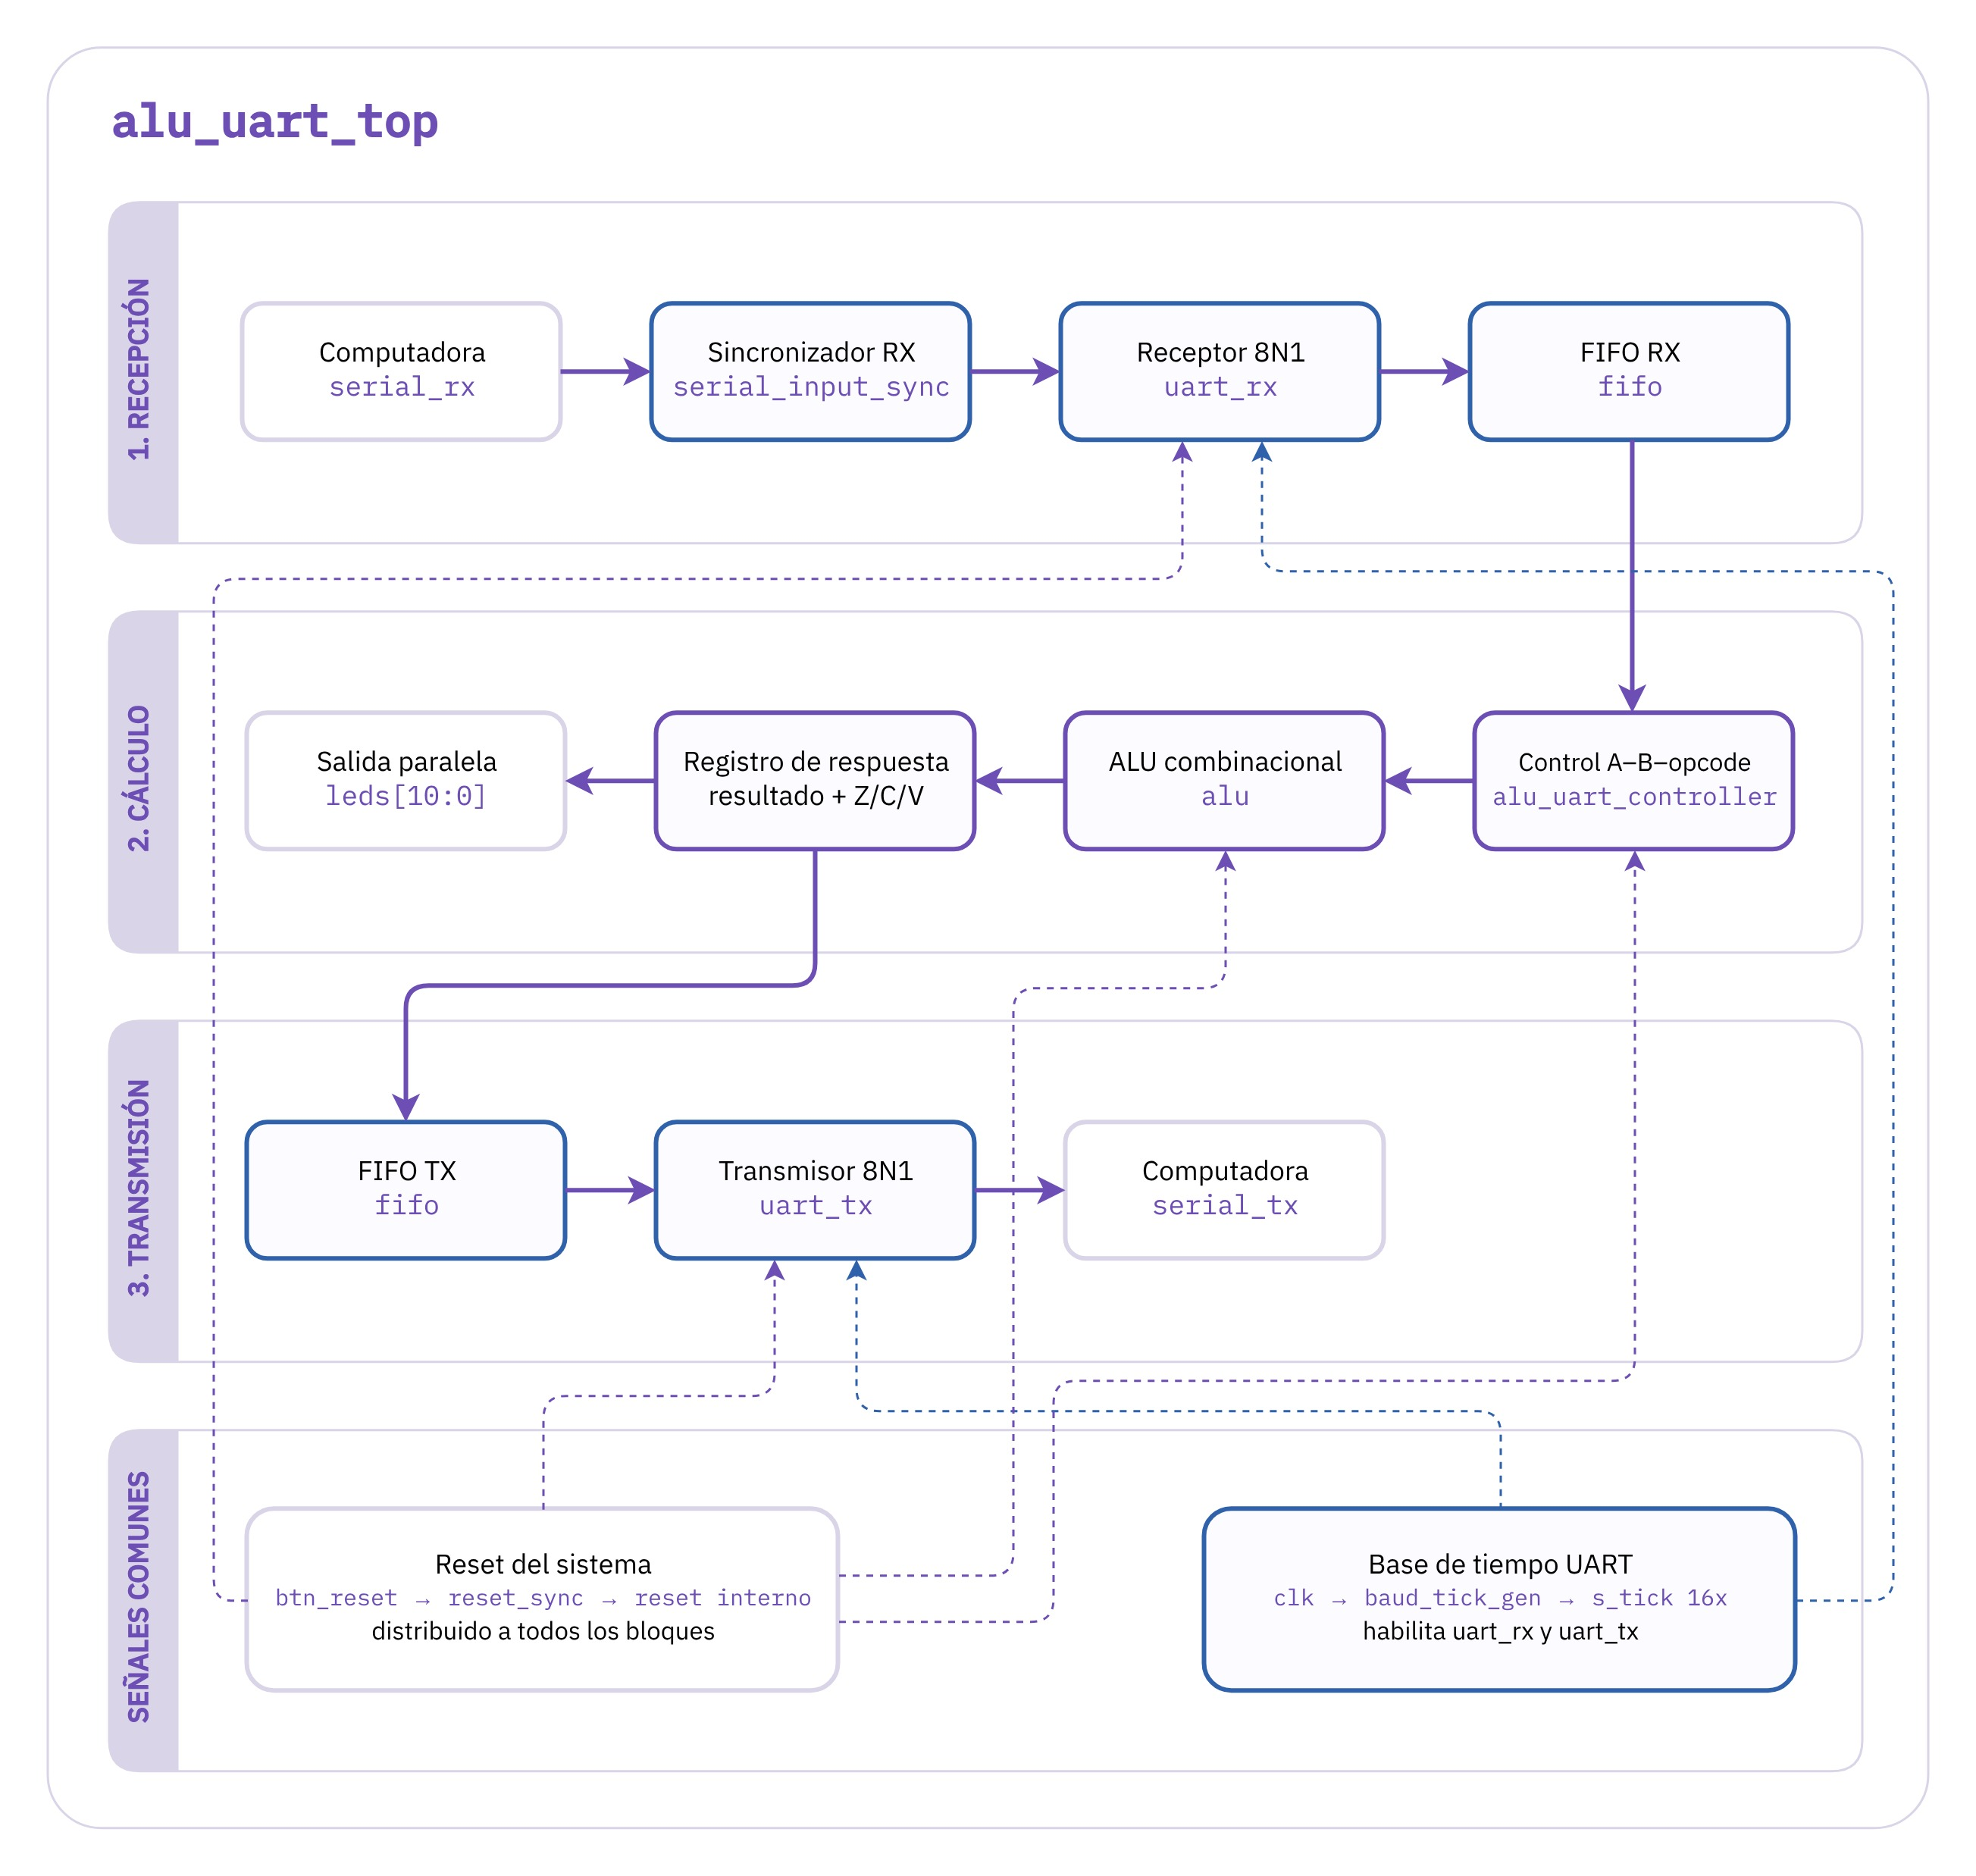
\includegraphics[width=0.88\textwidth]{img/architecture.jpg}
  \caption{Recorrido de los datos y separación funcional de la arquitectura.}%
  \label{fig:arquitectura-general}
\end{figure}

\clearpage

\newcommand{\moduleinterface}[4]{%
  \begin{figure}[H]
    \centering
    \begin{tikzpicture}[
        ifmodule/.style={draw=codeviolet,fill=codeback,rounded corners=2mm,
          minimum height=3.7cm,text width=4.5cm,align=center,thick,
        inner xsep=8pt,inner ysep=8pt,font=\normalsize},
        ifflow/.style={very thick,draw=codeviolet},
        iflabel/.style={font=\scriptsize,fill=white,inner sep=1.5pt}
      ]
      \node[ifmodule] (module) at (0,0)
      {{\color{technicalviolet}\bfseries\texttt{#1}}};
      \foreach \port/\height in {#2} {
        \draw[ifflow,-{Latex[length=2.6mm]}] (-6.6,\height) --
        node[iflabel,above] {\port} (-2.55,\height);
      }
      \foreach \port/\height in {#3} {
        \draw[ifflow,-{Latex[length=2.6mm]}] (2.55,\height) --
        node[iflabel,above] {\port} (6.6,\height);
      }
    \end{tikzpicture}
    \caption{Interfaz de #4.}%
  \end{figure}%
}

\subsection{Integración y acondicionamiento}

\texttt{alu\_uart\_top} es el módulo superior y representa el circuito conectado
a la placa. Expone únicamente el reloj de \SI{100}{\mega\hertz}, el pulsador de
reset, los pines \texttt{serial\_rx} y \texttt{serial\_tx}, y los once LED. Su
función no es procesar bits ni ejecutar operaciones: instancia los bloques
principales, les entrega los mismos parámetros de frecuencia y velocidad, y
conecta las interfaces de lectura y escritura entre el núcleo UART y el
controlador. Esta capa permite cambiar la implementación de una parte
sin alterar
los pines físicos del diseño.

\moduleinterface{alu\_uart\_top}
{{\texttt{clk}}/0.6,
  {\texttt{btn\_reset}}/0,
{\texttt{serial\_rx}}/-0.6}
{{\texttt{serial\_tx}}/0.35,
{\texttt{leds[10:0]}}/-0.35}
{\texttt{alu\_uart\_top}}

La entrada, al ser externa, puede cambiar sin relación con el reloj.
\texttt{reset\_sync} es el módulo que sincroniza ese cambio. Al
presionar el botón de reset, el reset interno se activa de inmediato;
al soltarlo, se mantiene activo durante dos flancos y recién entonces
se libera. De ese modo todos los módulos abandonan el reset sobre un
flanco conocido.

\moduleinterface{reset\_sync}
{{\texttt{clk}}/0.35,
{\texttt{async\_reset}}/-0.35}
{{\texttt{reset}}/0}
{\texttt{reset\_sync}}

\texttt{uart\_core} se ocupa de la comunicación serie. A partir de los bits que
llegan por \texttt{serial\_rx}, reconstruye cada byte y lo conserva hasta que el
controlador lo retira. En el sentido opuesto, recibe los bytes producidos por el
controlador y los transmite por \texttt{serial\_tx}.

De este modo, el controlador trabaja únicamente con bytes completos.
Las señales \texttt{rx\_empty} y \texttt{tx\_full} indican cuándo
puede leer o escribir, mientras que un pulso separado informa la
recepción de una trama inválida. Los detalles propios de UART, como
la duración y el orden de los bits o la comprobación del bit de stop,
permanecen contenidos dentro del núcleo.

\moduleinterface{uart\_core}
{{\texttt{clk}}/1.35,
  {\texttt{reset}}/0.81,
  {\texttt{serial\_rx}}/0.27,
  {\texttt{rd\_uart}}/-0.27,
  {\texttt{w\_data[7:0]}}/-0.81,
{\texttt{wr\_uart}}/-1.35}
{{\texttt{serial\_tx}}/1.08,
  {\texttt{r\_data[7:0]}}/0.54,
  {\texttt{rx\_empty}}/0,
  {\texttt{tx\_full}}/-0.54,
{\texttt{rx\_error\_tick}}/-1.08}
{\texttt{uart\_core}}

\subsection{Camino de recepción}

\texttt{serial\_input\_sync} adapta la entrada asíncrona
\texttt{serial\_rx} al reloj interno. Para ello hace pasar la señal por dos
flip-flops consecutivos y utiliza solamente la salida del segundo, lo que reduce
el riesgo de propagar metastabilidad. La salida sigue siendo un único bit, que
luego es procesado por la FSM receptora.

\moduleinterface{serial\_input\_sync}
{{\texttt{clk}}/0.6,
  {\texttt{reset}}/0,
{\texttt{serial\_async}}/-0.6}
{{\texttt{serial\_sync}}/0}
{\texttt{serial\_input\_sync}}

\texttt{baud\_tick\_gen} divide el reloj del sistema y produce
\texttt{s\_tick}, una habilitación de un ciclo a dieciséis veces la velocidad de
baud. No crea un reloj nuevo. RX y TX conservan el reloj de
\SI{100}{\mega\hertz}
y solo avanzan sus contadores cuando reciben ese pulso. Compartir el generador
mantiene una única referencia temporal para ambos sentidos de la comunicación.

\moduleinterface{baud\_tick\_gen}
{{\texttt{clk}}/0.35,
{\texttt{reset}}/-0.35}
{{\texttt{s\_tick}}/0}
{\texttt{baud\_tick\_gen}}

\texttt{uart\_rx} es el receptor del enlace UART. Su función es convertir la
secuencia recibida por la línea serie en bytes de ocho bits. Cuando completa una
trama 8N1 válida, coloca el byte en
\texttt{data\_out} y activa \texttt{rx\_done\_tick} durante un ciclo.
Si la trama
es inválida, descarta el dato y lo informa mediante
\texttt{frame\_error\_tick}. De este modo, los bloques siguientes reciben bytes
completos y una indicación explícita de éxito o error.

\moduleinterface{uart\_rx}
{{\texttt{clk}}/0.9,
  {\texttt{reset}}/0.3,
  {\texttt{rx}}/-0.3,
{\texttt{s\_tick}}/-0.9}
{{\texttt{data\_out[7:0]}}/0.6,
  {\texttt{rx\_done\_tick}}/0,
{\texttt{frame\_error\_tick}}/-0.6}
{\texttt{uart\_rx}}

\texttt{rx\_fifo} es la cola de recepción. Su función es conservar los bytes
entregados por \texttt{uart\_rx} hasta que el controlador pueda procesarlos. El
byte más antiguo queda disponible en \texttt{r\_data};
\texttt{rx\_empty} indica si la cola está vacía y \texttt{rd\_uart} retira el
dato leído. Si se recibe un byte cuando no queda espacio, \texttt{uart\_core}
informa el desbordamiento mediante \texttt{rx\_error\_tick}. Esta cola y la de
transmisión son dos instancias del mismo módulo paramétrico \texttt{fifo}.

\moduleinterface{fifo}
{{\texttt{clk}}/1.2,
  {\texttt{reset}}/0.6,
  {\texttt{rd}}/0,
  {\texttt{wr}}/-0.6,
{\texttt{write\_data[7:0]}}/-1.2}
{{\texttt{read\_data[7:0]}}/0.6,
  {\texttt{empty}}/0,
{\texttt{full}}/-0.6}
{la instancia \texttt{rx\_fifo}}

\subsection{Interpretación y cálculo}

\texttt{alu\_uart\_controller} es el módulo que interpreta el protocolo de la
aplicación y coordina la ejecución de la ALU. Recibe bytes completos desde
\texttt{uart\_core}, los organiza como operando A, operando B y
opcode, y entrega
el resultado al camino de transmisión. También conserva el resultado y las
banderas que se muestran en los LED. Si ocurre un error de recepción o vence el
timeout antes de completar una solicitud, descarta los datos parciales y espera
una transacción nueva.

\moduleinterface{alu\_uart\_controller}
{{\texttt{clk}}/1.35,
  {\texttt{reset}}/0.81,
  {\texttt{r\_data[7:0]}}/0.27,
  {\texttt{rx\_empty}}/-0.27,
  {\texttt{rx\_error\_tick}}/-0.81,
{\texttt{tx\_full}}/-1.35}
{{\texttt{rd\_uart}}/0.9,
  {\texttt{w\_data[7:0]}}/0.3,
  {\texttt{wr\_uart}}/-0.3,
{\texttt{leds[10:0]}}/-0.9}
{\texttt{alu\_uart\_controller}}

\texttt{alu} es el bloque combinacional que realiza las operaciones aritméticas
y lógicas. Recibe los operandos A y B junto con los seis bits del opcode, y
produce el resultado y las banderas zero, carry y overflow. El controlador
registra esas salidas para mantenerlas estables durante la transmisión y en los
LED. De este modo, la ALU se ocupa únicamente del cálculo y no interviene en la
comunicación UART.

\moduleinterface{alu}
{{\texttt{i\_data\_a[7:0]}}/0.6,
  {\texttt{i\_data\_b[7:0]}}/0,
{\texttt{i\_data\_opcode[5:0]}}/-0.6}
{{\texttt{o\_result[7:0]}}/0.9,
  {\texttt{o\_zero}}/0.3,
  {\texttt{o\_carry}}/-0.3,
{\texttt{o\_overflow}}/-0.9}
{\texttt{alu}}

\subsection{Camino de transmisión y salidas}

\texttt{tx\_fifo} es la cola de transmisión. Almacena los bytes producidos por
el controlador hasta que \texttt{uart\_tx} pueda enviarlos. El controlador
escribe mediante \texttt{w\_data} y \texttt{wr\_uart}, mientras que
\texttt{tx\_full} indica si existe espacio disponible. Cuando la cola está
llena, el controlador conserva el resultado y espera, evitando que se pierda la
respuesta.

\moduleinterface{fifo}
{{\texttt{clk}}/1.2,
  {\texttt{reset}}/0.6,
  {\texttt{rd}}/0,
  {\texttt{wr}}/-0.6,
{\texttt{write\_data[7:0]}}/-1.2}
{{\texttt{read\_data[7:0]}}/0.6,
  {\texttt{empty}}/0,
{\texttt{full}}/-0.6}
{la instancia \texttt{tx\_fifo}}

\texttt{uart\_tx} es el transmisor del enlace UART. Su función es convertir un
byte completo en una trama 8N1 y enviarla por la salida serie. La señal
\texttt{tx\_start} inicia la transmisión, \texttt{tx\_busy} indica que el módulo
está ocupado y \texttt{tx\_done\_tick} informa que la trama terminó. La salida
\texttt{tx} se conecta a \texttt{serial\_tx} en el nivel superior.

\moduleinterface{uart\_tx}
{{\texttt{clk}}/1.2,
  {\texttt{reset}}/0.6,
  {\texttt{tx\_start}}/0,
  {\texttt{s\_tick}}/-0.6,
{\texttt{data\_in[7:0]}}/-1.2}
{{\texttt{tx}}/0.6,
  {\texttt{tx\_done\_tick}}/0,
{\texttt{tx\_busy}}/-0.6}
{\texttt{uart\_tx}}

Los once LED se controlan de forma independiente al transmisor.
Muestran el resultado registrado y las banderas Z, C y V, por lo que
conservan su estado aunque la respuesta UART ya haya finalizado.

Esta distribución establece una regla clara entre módulos: el
productor solo escribe si la cola no está llena y el consumidor solo
lee si no está vacía. Las señales \texttt{wr}/\texttt{full} y
\texttt{rd}/\texttt{empty} convierten una relación temporal implícita
en un contrato verificable. Gracias a ello, cada bloque puede
probarse de manera aislada antes de comprobar el recorrido completo.

\section{Flujo de operación}

En reposo, las señales RX y TX permanecen en nivel alto, la cola de
recepción se encuentra vacía y el controlador espera el operando A.
Cuando llega una trama válida, RX entrega el byte recibido a la cola
de recepción. El controlador lo retira y pasa a esperar el operando
B; el proceso se repite para el opcode. En el estado correspondiente
la ALU ve los tres registros estables. Un ciclo después se capturan
el resultado y las banderas, y se espera a que haya capacidad
suficiente en la cola del transmisor.

La respuesta no se retira de la cola de transmisión cuando comienza a
transmitirse, sino al final del stop. En consecuencia, el dato
frontal permanece estable durante toda la trama. Si llega un error
antes de recibir los tres operandos, el controlador descarta los
registros parciales y el próximo byte vuelve a interpretarse como el
operando A. Esta regla evita asociar datos pertenecientes a
solicitudes distintas.

\section{Decisiones de diseño}

El protocolo con la computadora se mantuvo deliberadamente pequeño.
Cada solicitud está formada por tres bytes binarios enviados en un
orden fijo: primero el operando A, después el operando B y por último
el código de operación. Una vez recibida la terna, el circuito
responde con un único byte de resultado. Este formato evita
incorporar un analizador de texto, conversiones desde ASCII o
caracteres separadores, recursos que no contribuirían al objetivo del
trabajo. Como contrapartida, el emisor debe respetar el orden
acordado y el controlador debe recordar cuántos bytes válidos recibió
antes de ejecutar la ALU.

La UART opera a \num{19200} baud, una velocidad muy inferior al reloj
de \SI{100}{\mega\hertz} de la placa. Para relacionar ambas
velocidades, \texttt{baud\_tick\_gen} cuenta ciclos del reloj
principal y activa \texttt{s\_tick} cada 326 ciclos. De esta forma se
obtienen aproximadamente dieciséis instantes de referencia durante
cada bit de la trama UART.

El receptor y el transmisor continúan sincronizados con el reloj de
\SI{100}{\mega\hertz}, pero utilizan \texttt{s\_tick} para determinar
cuándo avanzar. Por lo tanto, \texttt{s\_tick} es una señal de
habilitación y no un segundo reloj. El receptor aprovecha esas
referencias para verificar el inicio de la trama y leer cada bit
cerca de su centro.

La recepción, la transmisión y la interpretación de una solicitud
avanzan por etapas y deben recordar cuál es la siguiente acción. Por
eso cada una se controla mediante una máquina de estados: RX, TX y el
controlador. Las tres utilizan codificación one-hot. Cada estado
posee su propio flip-flop: RX emplea cinco, TX cuatro y el
controlador otros cinco. Frente a una codificación binaria se
consumen más registros, pero en esta FPGA el costo es reducido y se
obtiene una relación directa entre cada estado y su bit de
representación. Esto simplifica el seguimiento de las transiciones
durante la simulación y permite reconocer con facilidad el estado
activo en los reportes de síntesis. El atributo \texttt{fsm\_encoding
= "one\_hot"} deja explícita esa elección, y la rama por defecto de
cada FSM define además un retorno seguro si el registro de estado
adopta una combinación inválida.

Los FIFO resuelven la diferencia de ritmo entre la comunicación UART
y el procesamiento interno. Se eligió una profundidad de cuatro bytes
porque alcanza para absorber una ráfaga breve sin convertir las colas
en memoria para una sesión completa. En recepción, cada trama válida
ocupa una posición hasta que el controlador la retira; si llega un
nuevo byte con las cuatro posiciones ocupadas, el núcleo no
sobrescribe información previa y notifica el desbordamiento
(\textit{overrun}). En transmisión, la situación se resuelve mediante
espera: si \texttt{tx\_full} está activo, el controlador conserva el
resultado y sus banderas hasta que exista una posición libre. El
registro de respuesta también mantiene estables los LED y evita que
una solicitud parcial modifique el último resultado válido.

El orden fijo de tres bytes plantea un último problema: si la
computadora envía A o A--B y luego interrumpe la transferencia, el
controlador no puede conservar esa solicitud incompleta de manera
indefinida. Por ese motivo se incorporó un tiempo máximo de espera
(\textit{timeout}) de \SI{10}{\milli\second}. A \num{19200} baud, una
trama 8N1 dura aproximadamente \SI{0.521}{\milli\second}, de modo que
el margen admite pausas considerablemente mayores que el tiempo de
transmisión normal. Si el plazo vence o RX informa un error antes de
completar la terna, se descartan los registros parciales y el
siguiente byte vuelve a interpretarse como el operando A.

En conjunto, estas decisiones priorizan un comportamiento
determinista y verificable. Cada bloque posee una condición explícita
para aceptar datos, esperar o recuperarse, sin depender de retardos
implícitos entre módulos.

\section{Organización del proyecto}

El árbol de la figura~\ref{fig:jerarquia-modulos} refleja la
jerarquía sintetizable, no solo la distribución de
archivos.\ \texttt{alu\_uart\_top} instancia el acondicionador de
reset, el núcleo UART y el controlador. Dentro del núcleo quedan
sincronizador, generador, receptor, transmisor y ambos FIFO; dentro
del controlador se conserva la ALU del TP1.

\begin{figure}[H]
  \centering
  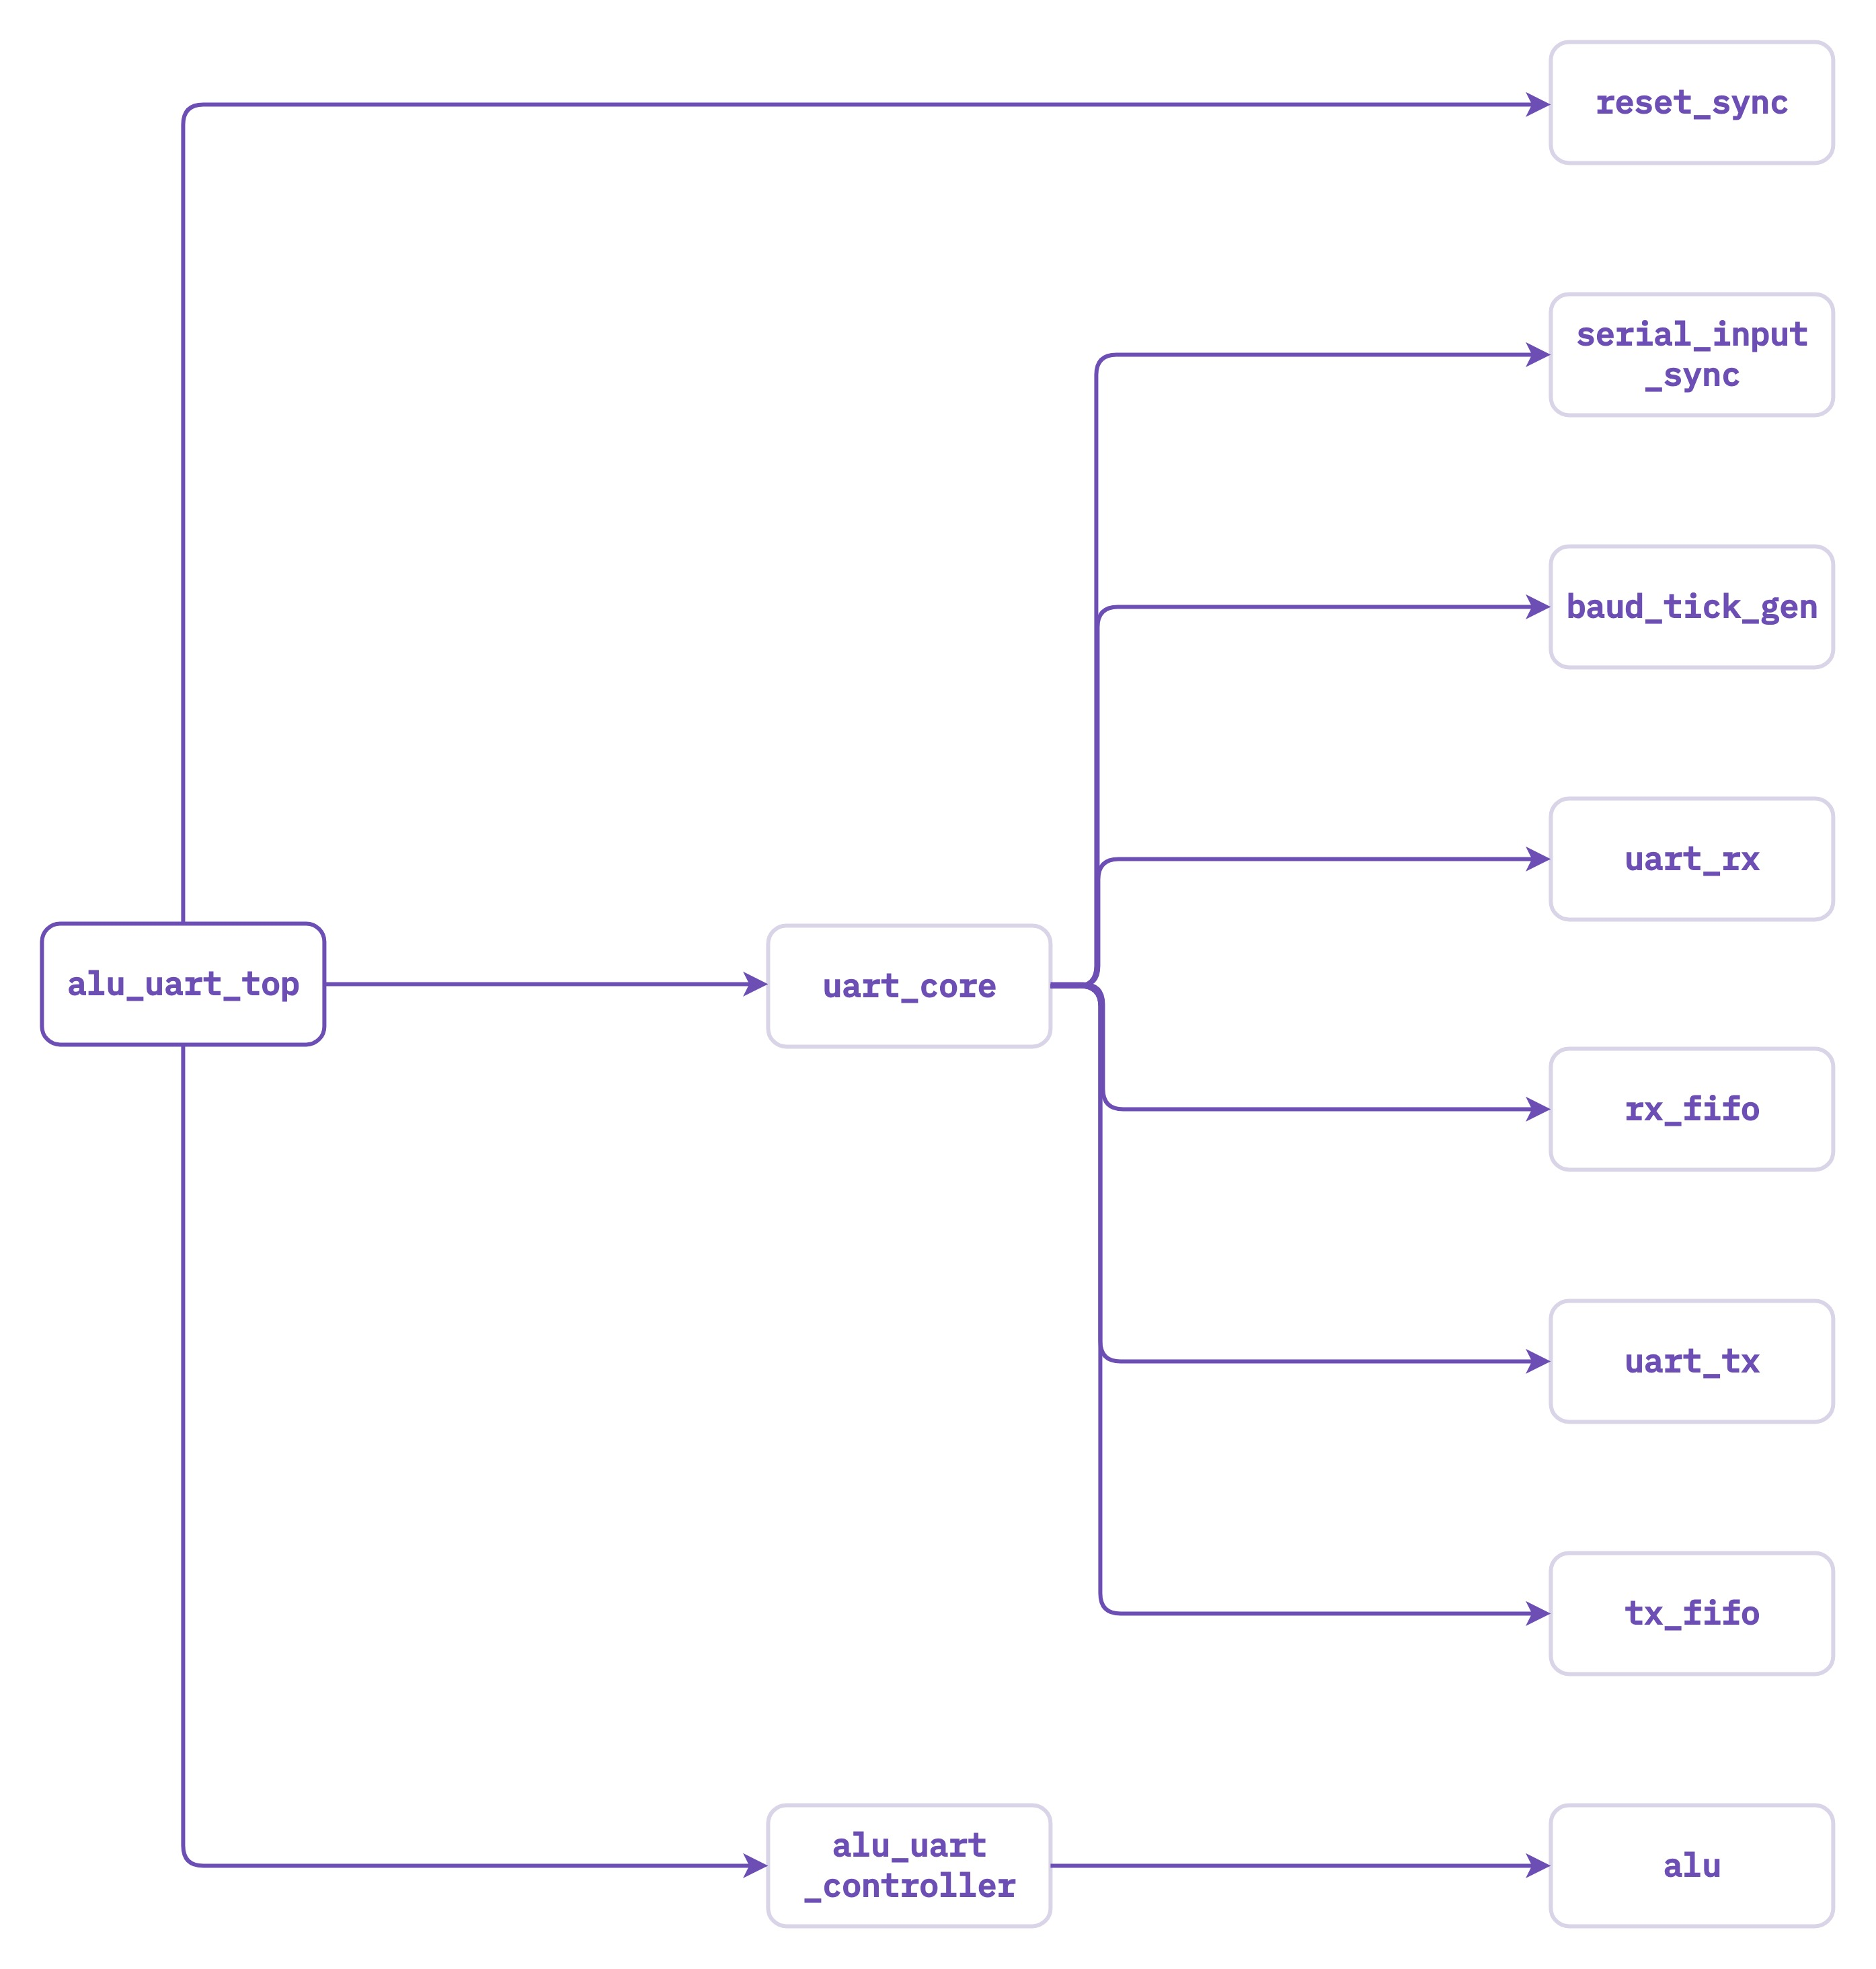
\includegraphics[height=10.8cm,keepaspectratio]{img/modules.jpg}
  \caption{Jerarquía de módulos elaborada a partir de las instancias RTL.}%
  \label{fig:jerarquia-modulos}
\end{figure}


\chapter{Núcleo UART y máquinas de estado}\label{chap:nucleo-uart}
\section{Contrato del enlace y formato UART 8N1}

En el TP1, cada operando llegaba a la ALU mediante ocho señales
paralelas: una por cada bit. En este trabajo, la computadora envía
esos mismos ocho bits de forma secuencial mediante UART. Los bits de
cada byte ingresan uno después de otro por RX y la respuesta se
transmite del mismo modo por TX. Como UART no incorpora una señal de
reloj, la computadora y la FPGA deben utilizar la misma velocidad y
el mismo formato de trama. En este diseño se emplean \num{19200} baud
y el formato 8N1: ocho bits de datos, sin paridad y con un bit de stop.

Cada byte ocupa diez períodos de bit. Mientras no hay una
transmisión, RX y TX permanecen en nivel alto. Un bit de start en
bajo marca el comienzo de la trama; a continuación se envían los ocho
bits de datos, desde el menos significativo hasta el más
significativo, y un bit de stop en alto indica el final.

\begin{figure}[H]
  \centering
  \begin{tikzpicture}[
      x=1.05cm,y=0.8cm,
      lbl/.style={font=\small,align=center}
    ]
    \draw[->,thick] (-0.35,0) -- (10.55,0);
    \foreach \x in {0,...,10} {
      \draw[gray!55] (\x,-0.15) -- (\x,1.2);
    }
    \draw[very thick,codeviolet]
    (-0.3,1) -- (0,1) -- (0,0.2) -- (1,0.2);
    \draw[very thick,codeviolet]
    (1,0.2) -- (1,0.82) -- (2,0.82) -- (2,0.2) --
    (3,0.2) -- (3,0.82) -- (4,0.82) -- (4,0.2) --
    (5,0.2) -- (5,0.82) -- (6,0.82) -- (6,0.2) --
    (7,0.2) -- (7,0.82) -- (8,0.82) -- (8,0.2) --
    (9,0.2) -- (9,1) -- (10.4,1);
    \node[lbl] at (0.5,-0.42) {start};
    \foreach \x in {0,...,7} {
      \node[lbl] at ({1.5+\x},-0.42) {D\x};
    }
    \node[lbl] at (9.5,-0.42) {stop};
    \draw[<->,codeblue] (0,1.37) -- node[above,lbl]
    {$T_{\mathrm{bit}}$} (1,1.37);
  \end{tikzpicture}
  \caption{Estructura temporal de una trama UART 8N1.}%
  \label{fig:trama-uart}
\end{figure}

Las líneas verticales de la figura~\ref{fig:trama-uart} delimitan
diez intervalos iguales. El primer nivel bajo no es parte del dato:
permite al receptor detectar el inicio. D0 llega antes que D7, por lo
que el orden temporal no coincide con la forma habitual de escribir
un byte. El stop alto confirma el final y devuelve la línea a su
nivel de reposo.

A \num{19200} baud, un bit dura aproximadamente
\SI{52.083}{\micro\second} y cada byte ocupa
\SI{520.833}{\micro\second}. El envío de los tres bytes de entrada
demanda al menos \SI{1.563}{\milli\second}; la respuesta agrega otro
intervalo de byte. Estos valores no incluyen demoras del sistema
operativo o del adaptador USB.

\section{Generación del tick de muestreo}

El receptor utiliza sobremuestreo 16x: por cada bit recibido se
generan dieciséis pulsos de muestreo. De este modo, cada período de
bit queda dividido en dieciséis intervalos que sirven como referencia
temporal. Después de detectar la transición que puede indicar un bit
de start, el receptor espera ocho pulsos para comprobar su valor
cerca del centro. Si el start es válido, toma una muestra de cada bit
de datos cada dieciséis pulsos y finalmente hace lo mismo con el bit de stop.

Para obtener esos dieciséis pulsos por bit, el generador produce
\texttt{s\_tick} a una frecuencia 16 veces mayor que la tasa UART:

\begin{equation}
  f_{\mathrm{tick}} = 16 \cdot 19200 =
  \SI{307200}{\hertz}.
\end{equation}

Como el reloj de la placa es de \SI{100}{\mega\hertz}, se utiliza un
divisor entero redondeado al valor más próximo:

\begin{equation}
  D = \operatorname{round}
  \left(\frac{100\,000\,000}{307\,200}\right) = 326.
\end{equation}

El resultado no es exacto. El tick real es \SI{306748.466}{\hertz} y
la tasa efectiva es \SI{19171.779}{baud}, con un error relativo de
aproximadamente \SI{-0.147}{\percent}. La diferencia acumulada a lo
largo de una trama es muy inferior a medio bit y queda dentro del
margen que ofrece el muestreo central.

El RTL conserva el reloj de \SI{100}{\mega\hertz} y genera un pulso
de habilitación cada 326 ciclos. La suma de media frecuencia antes de
la división implementa el redondeo entero.

% tex-fmt: off
\begin{codebox}[language=SystemVerilog]
localparam integer TICK_FREQ_HZ = BAUD_RATE * OVERSAMPLE;
localparam integer DIVISOR =
  (CLK_FREQ_HZ + (TICK_FREQ_HZ / 2)) / TICK_FREQ_HZ;

always @(posedge clk) begin
  if (reset) begin
    counter <= '0;
    s_tick  <= 1'b0;
  end else if (counter == DIVISOR - 1) begin
    counter <= '0;
    s_tick  <= 1'b1;
  end else begin
    counter <= counter + 1'b1;
    s_tick  <= 1'b0;
  end
end
\end{codebox}
% tex-fmt: on

El fragmento muestra qué hardware se obtiene: un contador, un
comparador contra 325 y un registro para el pulso. Como
\texttt{s\_tick} permanece bajo en todos los demás ciclos, RX y TX
avanzan sus contadores de sub-bit únicamente cuando corresponde, pero
todos sus registros siguen capturados por \texttt{clk}.

\section{Protocolo de aplicación}

Cada operación tiene longitud fija. La computadora transmite A, luego
B y por último el opcode. Una vez recibidos los tres bytes válidos,
la FPGA responde con un byte de resultado.

\begin{table}[H]
  \centering
  \begin{tabularx}{0.94\textwidth}{ZZZZZ}
    \toprule
    \textbf{Sentido} & \textbf{Byte 0} & \textbf{Byte 1} &
    \textbf{Byte 2} & \textbf{Respuesta} \\
    \midrule
    PC a FPGA & A, 8 bits & B, 8 bits &
    Opcode en bits 5--0 & --- \\
    FPGA a PC & --- & --- & --- & Resultado, 8 bits \\
    \bottomrule
  \end{tabularx}
  \caption{Orden de los bytes del protocolo binario.}%
\end{table}

Los bits 7 y 6 del tercer byte se ignoran. Esta elección permite
enviar el opcode dentro de una palabra UART completa sin agregar
codificación ASCII. El protocolo es deliberadamente mínimo: no se
devuelve un byte separado de estado porque el requisito funcional
solicita el resultado y las banderas continúan visibles en LED8, LED9 y LED10.

\begin{table}[H]
  \centering
  \begin{tabular}{lccc}
    \toprule
    \textbf{Operación} & \textbf{Opcode} & \textbf{Hexadecimal} &
    \textbf{Resultado} \\
    \midrule
    SRA & \texttt{000011} & \texttt{03} & A desplazado aritméticamente
    B lugares \\
    SRL & \texttt{000010} & \texttt{02} & A desplazado lógicamente B lugares \\
    ADD & \texttt{100000} & \texttt{20} & A + B \\
    SUB & \texttt{100010} & \texttt{22} & A - B \\
    AND & \texttt{100100} & \texttt{24} & A AND B \\
    OR  & \texttt{100101} & \texttt{25} & A OR B \\
    XOR & \texttt{100110} & \texttt{26} & A XOR B \\
    NOR & \texttt{100111} & \texttt{27} & NOT (A OR B) \\
    \bottomrule
  \end{tabular}
  \caption{Operaciones conservadas del TP1.}%
\end{table}

Por ejemplo, para calcular \texttt{7F + 01}, el host transmite
\texttt{7F 01 20}. La respuesta esperada es \texttt{80}; al mismo
tiempo, LED10 se enciende para indicar overflow y los LED de carry y
cero permanecen apagados.

\section{Recuperación y casos inválidos}

El controlador debe volver a su estado inicial si la computadora deja
de enviar datos antes de completar una solicitud. Una vez recibido A,
o A y B, espera como máximo \SI{10}{\milli\second} el byte siguiente.
Si vence ese plazo, descarta la operación parcial y el próximo byte
se interpreta nuevamente como A. El timeout supera ampliamente los
\SI{0.521}{\milli\second} de una trama normal, aun cuando los bytes
se envían de manera individual.

\begin{table}[H]
  \centering
  \begin{tabularx}{\textwidth}{L{4.0cm}L{4.6cm}Y}
    \toprule
    \textbf{Situación} & \textbf{Acción} & \textbf{Respuesta} \\
    \midrule
    Start vuelve a alto antes del centro & Abortar la trama y esperar
    reposo alto. & Ninguna. \\
    Stop bajo & Emitir error de trama y esperar reposo alto. & Ninguna. \\
    FIFO RX lleno & Conservar los cuatro bytes previos y notificar
    overrun. & Se aborta la transacción parcial. \\
    Transacción incompleta & Vencer el contador a los
    \SI{10}{\milli\second}. & Ninguna. \\
    Opcode no reconocido & Ejecutar el caso por defecto de la ALU. &
    Un byte \texttt{00}, con Z activo. \\
    FIFO TX lleno & Conservar resultado e indicadores. & Esperar espacio
    antes de encolar. \\
    \bottomrule
  \end{tabularx}
  \caption{Política de tratamiento de condiciones excepcionales.}%
\end{table}

\section{Estructura y codificación de las máquinas de estado}

Como se anticipó al describir la arquitectura, la recepción, la
transmisión y el control de cada operación avanzan por etapas y
necesitan conservar su progreso entre ciclos de reloj. Por ese motivo
se utilizaron tres máquinas de estado: RX, TX y el controlador.

Las tres FSM comparten la misma estructura: un registro de estado,
lógica combinacional para determinar el próximo estado y las salidas,
constantes locales para representar cada etapa y una rama
\texttt{default} que permite regresar a IDLE ante una codificación no
contemplada.

Se eligió la codificación one-hot para las tres FSM. En este tipo de
codificación cada estado ocupa un flip-flop y solo un bit debe
permanecer activo. Esta representación consume más registros que una
codificación binaria, pero simplifica la lógica de decodificación en
FPGA y hace visibles los estados durante la depuración. RX utiliza
cinco bits, TX cuatro y el controlador cinco. El atributo
\texttt{fsm\_encoding = one\_hot} conserva esta intención durante la
extracción y optimización de las máquinas en Vivado.

En una codificación binaria cinco estados requerirían tres bits y
cada transición debería decodificar una combinación. En la
codificación one-hot se reservan cinco bits, por ejemplo
\texttt{00001} para IDLE y \texttt{00100} para DATA. El costo
adicional es de dos flip-flops; la ventaja es que comprobar ``estoy
en DATA'' se reduce conceptualmente a observar un solo bit. Esto no
elimina la necesidad de describir qué ocurre ante \texttt{00000} o
ante dos bits activos: la rama \texttt{default} devuelve la FSM al estado IDLE.

% tex-fmt: off
\begin{codebox}[language=SystemVerilog]
(* fsm_encoding = "one_hot" *) reg [4:0] state = STATE_IDLE;
reg [4:0] next_state;

always @(posedge clk) begin
  if (reset)
    state <= STATE_IDLE;
  else
    state <= next_state;
end

always_comb begin
  next_state = state;
  case (state)
    // cada estado modifica solo las senales necesarias
    default: next_state = STATE_IDLE;
  endcase
end
\end{codebox}
% tex-fmt: on

El registro secuencial \texttt{state} representa el estado actual. El
bloque combinacional calcula el próximo estado \texttt{next\_state} y
las salidas a partir de entradas y registros.

\section{Receptor UART}

La FSM del receptor separa reposo, validación del bit de start,
recepción de los datos, validación del bit de stop y recuperación.
Sus transiciones principales se resumen en la figura~\ref{fig:fsm-rx}.

\begin{figure}[H]
  \centering
  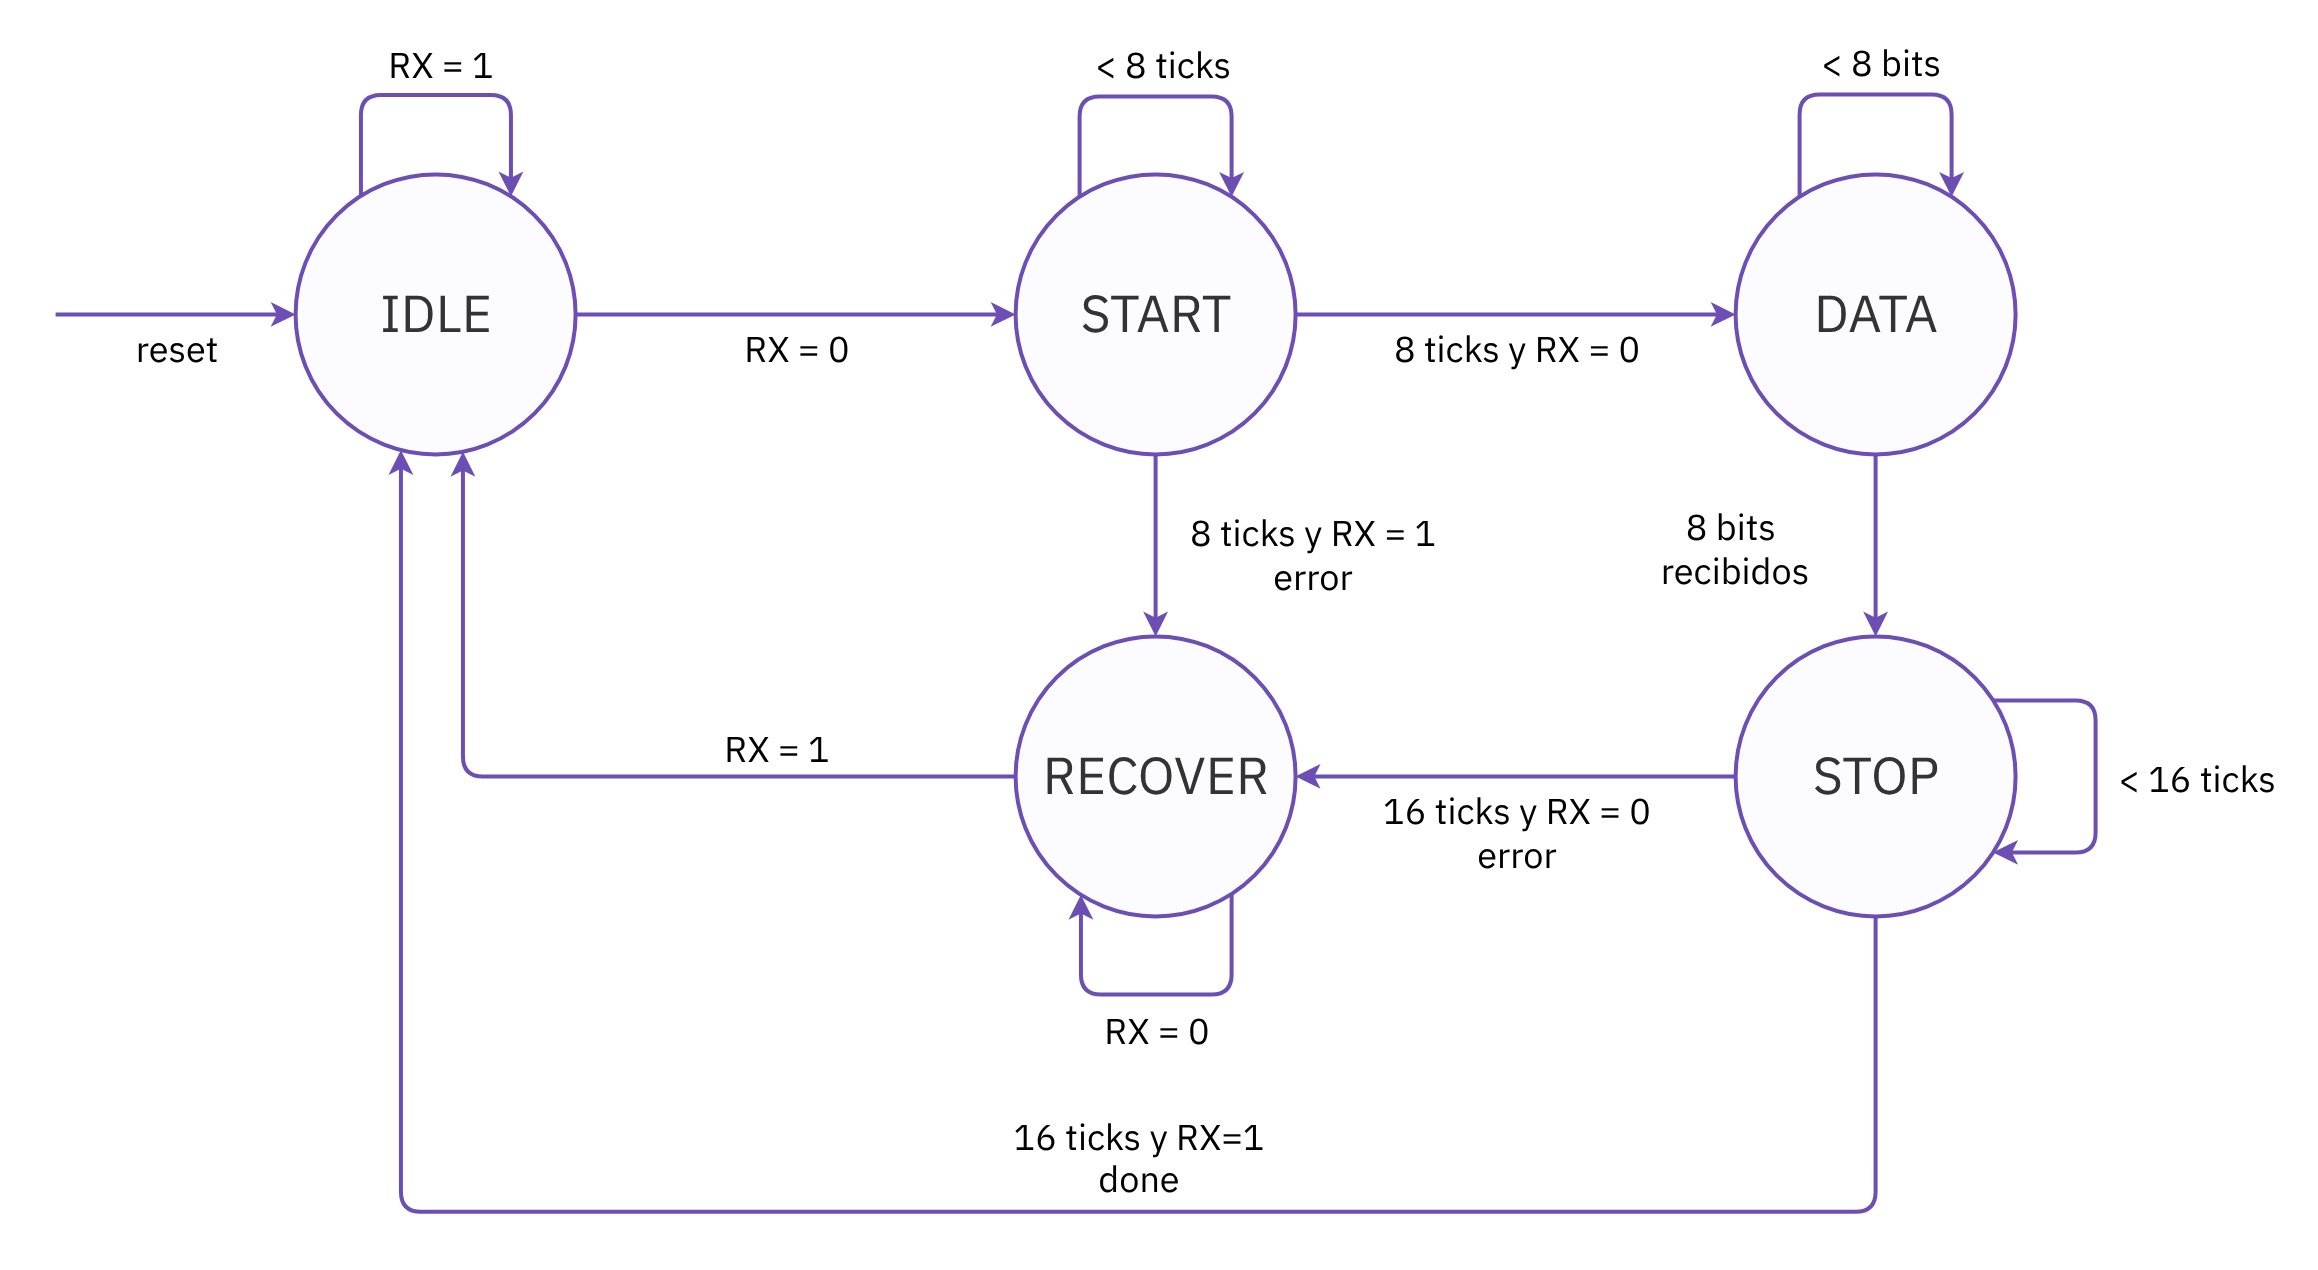
\includegraphics[width=0.94\textwidth]{img/fsm_rx.jpg}
  \caption{Estados y condiciones principales del receptor.}%
  \label{fig:fsm-rx}
\end{figure}

\subsection{Validación del bit de start}

En IDLE, una entrada baja inicia la observación. La FSM no la acepta
de inmediato si no que espera ocho ticks, es decir, medio período de
bit para sobremuestreo 16x. Si RX continúa bajo, el punto observado
corresponde al centro del start y se pasa a DATA. Si volvió a alto,
se trata de un pulso espurio por lo que se genera un único
\texttt{frame\_error\_tick} y se ingresa en RECOVER.

\subsection{Muestreo y orden de bits}

Después del centro del start, cada dato se toma al completar
dieciséis ticks. Como UART envía D0 primero, la nueva muestra entra
por el bit más significativo de un registro que se desplaza a la derecha:

% tex-fmt: off
\begin{codebox}[language=SystemVerilog]
next_data = {rx, data_reg[DATA_BITS-1:1]};
\end{codebox}
% tex-fmt: on

Tras ocho iteraciones, las muestras quedan en su posición natural. Se
espera entonces un período completo de stop. Solo si RX es alto se
genera \texttt{rx\_done\_tick}; un stop bajo no publica el byte.

\subsection{Estado de recuperación}

Después de un falso start o de un stop inválido, la línea puede
permanecer baja durante varios bits. Si se volviera inmediatamente a
IDLE se generaría un error repetido por cada nueva observación de ese
mismo nivel. RECOVER mantiene los contadores en cero y espera el
retorno a reposo en alto antes de habilitar otra trama. Así, cada
evento defectuoso produce un solo pulso de error.

\section{Transmisor UART}

El transmisor recibe un byte completo, pero debe enviarlo por
\texttt{tx} un bit a la vez y respetar la duración de cada parte de
la trama 8N1. Una máquina de estados conserva el avance de esa
secuencia. Como todos los niveles de salida son generados por el
propio circuito, se requieren cuatro estados: IDLE, START, DATA y STOP.

En IDLE, la línea permanece en alto. Un pulso en \texttt{tx\_start}
hace que el módulo guarde \texttt{data\_in} y comience el bit de
start en nivel bajo. Luego transmite los ocho bits de datos desde D0
hasta D7 y finaliza con el bit de stop en alto. Cada bit se mantiene
durante dieciséis pulsos de \texttt{s\_tick}.

\begin{figure}[H]
  \centering
  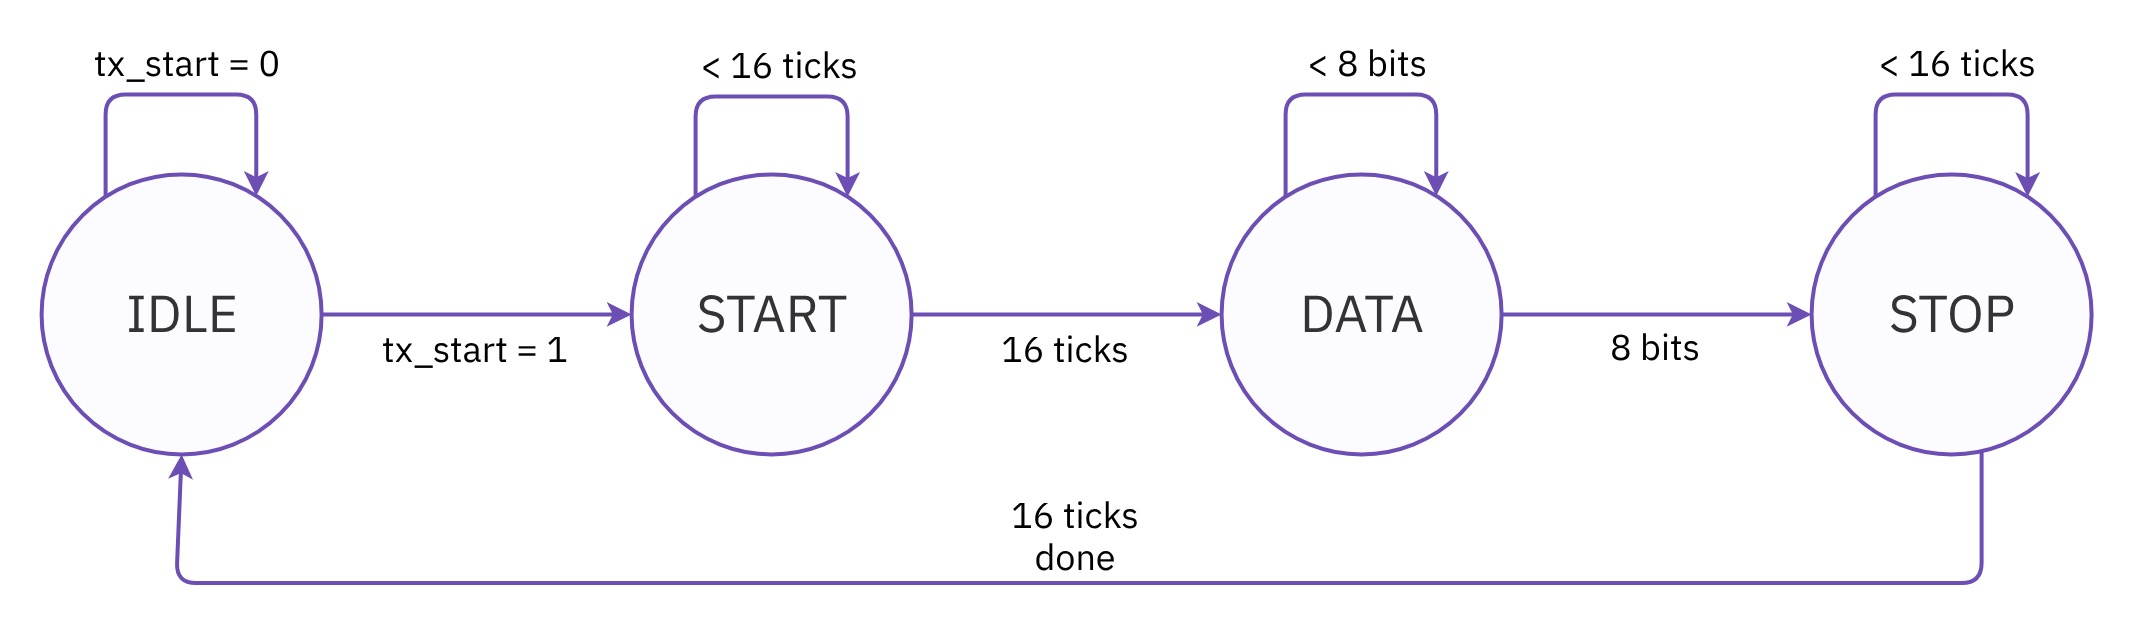
\includegraphics[width=0.86\textwidth]{img/fsm_tx.jpg}
  \caption{Secuencia de estados del transmisor.}%
\end{figure}

Mientras la trama está en curso, \texttt{tx\_busy} permanece activo.
Al completar el stop, \texttt{tx\_done\_tick} se activa durante un
ciclo y permite que el núcleo retire el byte del FIFO. Si todavía
quedan datos pendientes, una nueva activación de \texttt{tx\_start}
inicia la trama siguiente.

El byte se copia a un registro interno al comenzar la transmisión.
Así conserva el mismo valor durante toda la trama, aunque
\texttt{data\_in} cambie antes de que finalice. Al terminar cada
período de bit, el registro se desplaza para presentar el dato siguiente:

% tex-fmt: off
\begin{codebox}[language=SystemVerilog]
if (tx_start) begin
  next_state = STATE_START;
  next_data  = data_in;
  next_tx    = 1'b0;
end
// ... al terminar cada dato
next_data = {1'b0, data_reg[DATA_BITS-1:1]};
next_tx   = data_reg[1];
\end{codebox}
% tex-fmt: on

\section{Buffers FIFO}

La UART y el controlador no siempre están listos en el mismo ciclo.
El FIFO se ubica entre ambos y conserva temporalmente los bytes, de
modo que el productor puede escribir sin esperar que el consumidor
los retire de inmediato. Una escritura se acepta mientras exista
espacio y una lectura, mientras haya datos disponibles.

Cada FIFO puede almacenar cuatro bytes. El registro
\texttt{read\_pointer} señala el byte que se leerá a continuación,
mientras que \texttt{write\_pointer} indica la posición de la próxima
escritura. Ambos avanzan de forma circular: después de la última
posición regresan a la primera.

El registro \texttt{count} indica cuántos bytes contiene la cola.
Este valor permite distinguir entre vacío y lleno incluso cuando los
dos punteros coinciden. Si una lectura y una escritura se aceptan en
el mismo ciclo, sale un byte y entra otro, por lo que la cantidad de
datos almacenados no cambia.

% tex-fmt: off
\begin{codebox}[language=SystemVerilog]
assign empty = (count == 0);
assign full  = (count == DEPTH);
assign read_accept  = rd && !empty;
assign write_accept = wr && !full;

case ({write_accept, read_accept})
  2'b10:   count <= count + 1'b1;
  2'b01:   count <= count - 1'b1;
  default: count <= count;
endcase
\end{codebox}
% tex-fmt: on

Si la cola está llena al comenzar el ciclo, no puede aceptar una
nueva escritura, aunque \texttt{rd} y \texttt{wr} se activen al mismo
tiempo. En ese flanco se realiza solamente la lectura, que libera una
posición. La escritura puede repetirse en el ciclo siguiente, cuando
ya existe espacio disponible. De esta forma se evita sobrescribir el
dato más antiguo. Este caso también se comprueba en \texttt{fifo\_tb}.

\section{Controlador de transacciones}\label{sec:controlador-transacciones}

La tercera FSM traduce bytes completos al contrato de la ALU. En el
estado WAIT\_A consume el primer elemento de la cola de recepción y
carga el operando A. En los estados WAIT\_B y WAIT\_OPCODE se hace lo
mismo para el operando B y el opcode. El estado de EXECUTE reserva un
ciclo para registrar el resultado y mostrar los indicadores. El
estado de WAIT\_TX conserva esos registros si la cola de transmisión
está llena y escribe cuando existe espacio en la misma.

\begin{figure}[H]
  \centering
  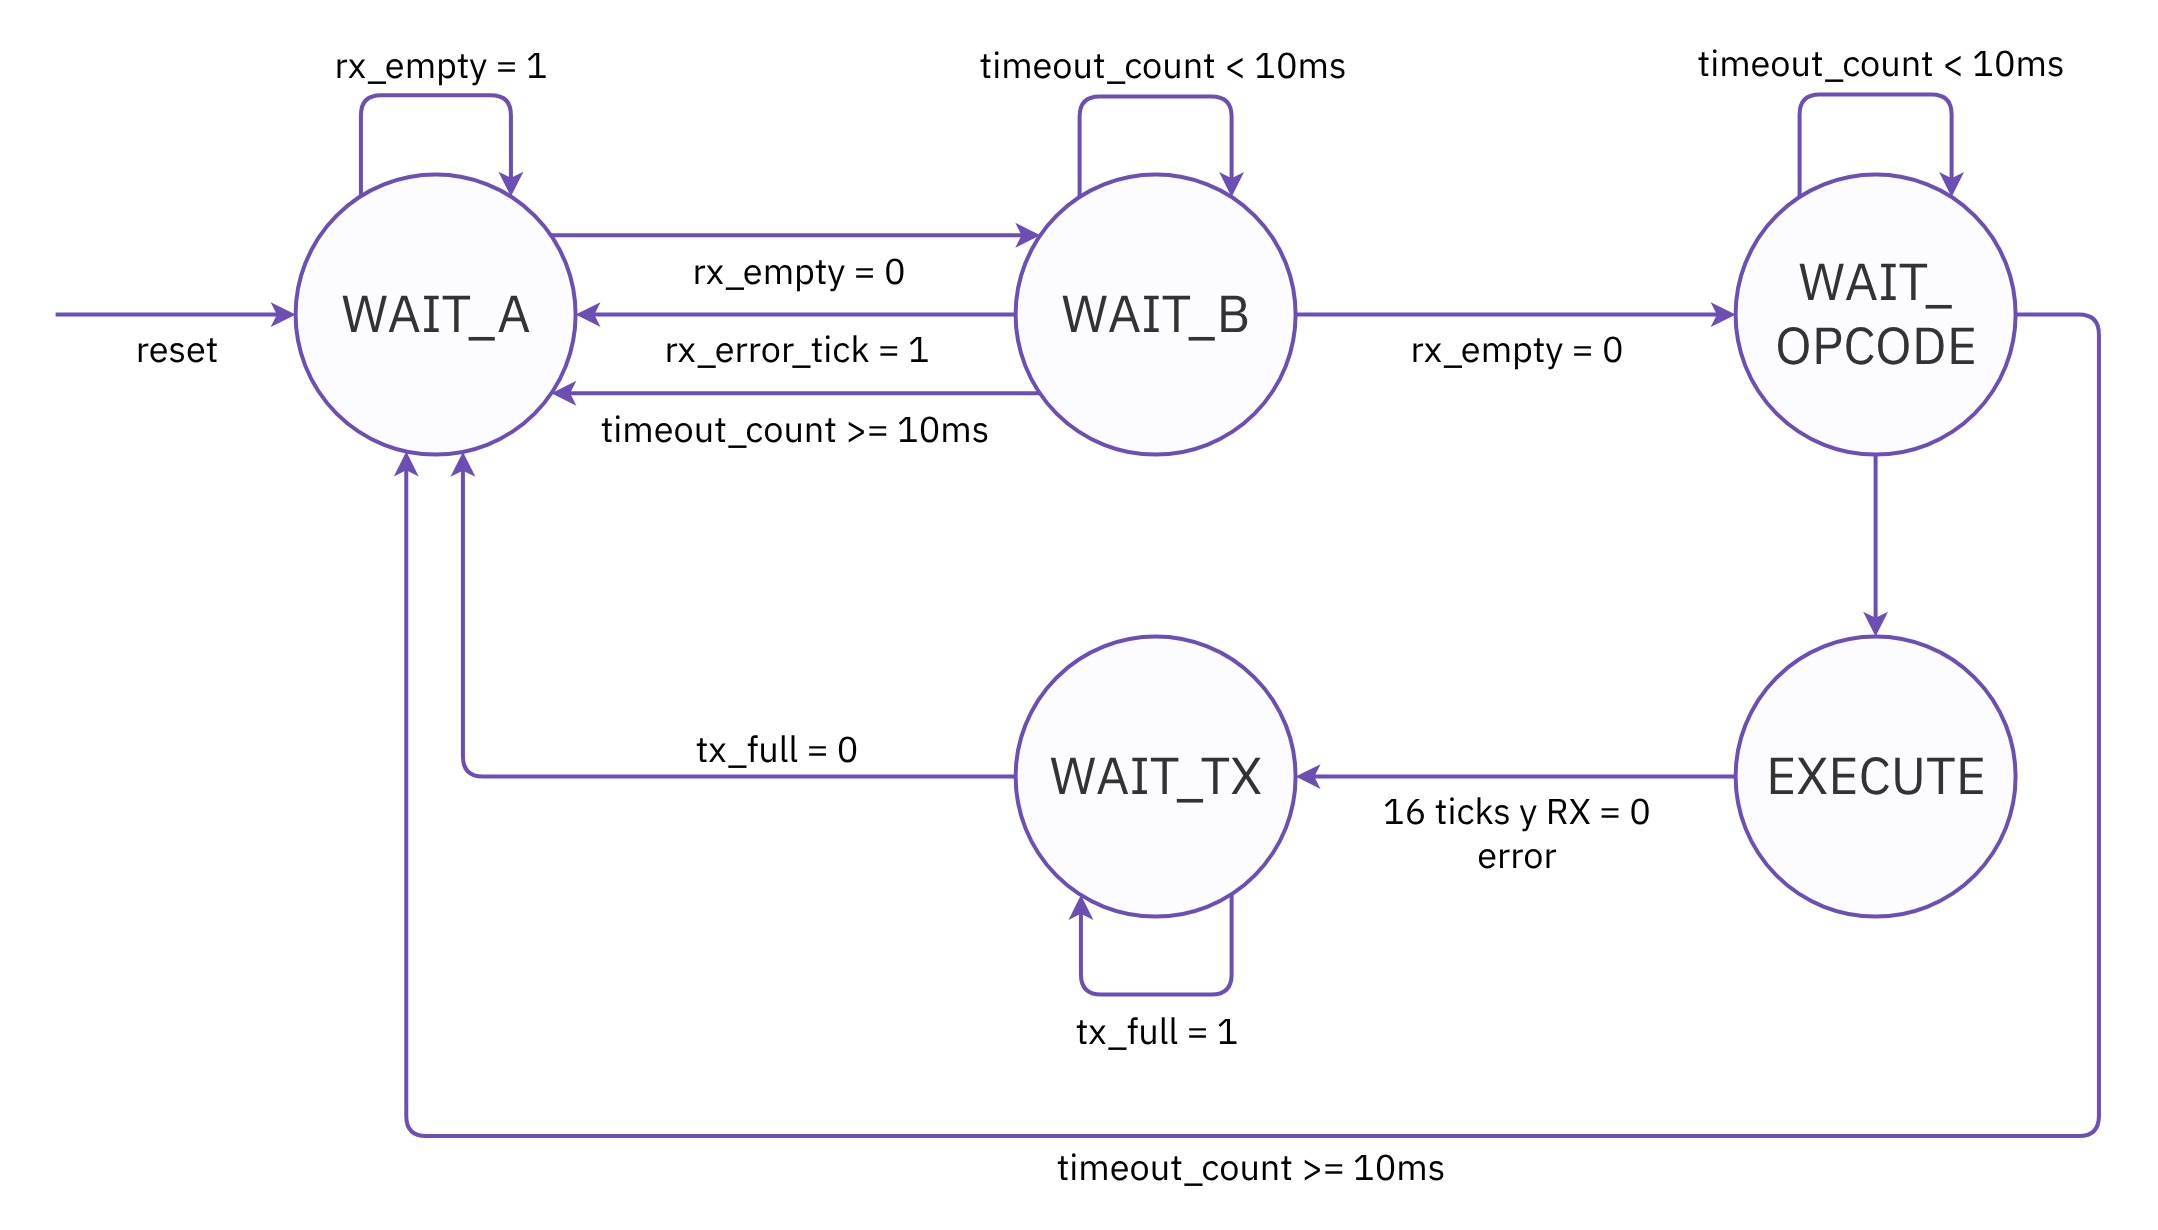
\includegraphics[width=0.875\textwidth]{img/fsm_controller.jpg}
  \caption{FSM que delimita una operación de tres bytes.}%
\end{figure}

El timeout solo es necesario después de recibir el primer operando y
antes de completar la solicitud. Por eso el contador avanza mientras
el controlador espera B o el opcode, y vuelve a cero cada vez que
llega un byte válido. Mientras se espera A permanece inactivo. Si
vence el plazo o RX informa un error durante una solicitud parcial,
los datos recibidos se descartan y el controlador vuelve a WAIT\_A.

Cuando llega el opcode, su registro se actualiza al finalizar el
flanco de reloj. El resultado de la ALU no puede capturarse en ese
mismo instante porque todavía depende del valor anterior. El estado
EXECUTE proporciona un ciclo adicional para que A, B y opcode
permanezcan estables y la ALU produzca el resultado correcto.
Después, WAIT\_TX conserva ese resultado y sus banderas hasta que
haya espacio en la cola de transmisión.

% tex-fmt: off
\begin{codebox}[language=SystemVerilog]
STATE_EXECUTE: begin
  capture_result = 1'b1;
  next_state = STATE_WAIT_TX;
end

STATE_WAIT_TX: begin
  if (!tx_full) begin
    wr_uart = 1'b1;
    next_state = STATE_WAIT_A;
  end
end
\end{codebox}
% tex-fmt: on

\section{Recuperación de estados ilegales}

En una codificación one-hot, solo son válidas las combinaciones que
tienen un único bit activo. Una perturbación podría modificar el
registro y producir una combinación que no represente ningún estado
definido. Para evitar que la máquina quede detenida en esa situación,
cada sentencia \texttt{case} incluye una rama \texttt{default}.

Ante un estado no reconocido, las FSM de RX y TX regresan a IDLE y
restablecen sus registros auxiliares. El controlador vuelve a WAIT\_A
para comenzar una solicitud nueva. De este modo, todas las
combinaciones posibles conducen a un comportamiento definido y la
operación puede continuar desde un estado conocido en el ciclo siguiente.


\chapter{Integración con la ALU y la Basys 3}
El sistema se utiliza desde una computadora conectada al puerto USB--UART de la
Basys 3. Desde allí se envían los operandos y el opcode de cada operación. La
placa procesa esos valores y devuelve el resultado por el mismo enlace.

Los datos no pasan directamente desde la computadora hasta la ALU. Primero se
transmiten por UART como una secuencia de tres bytes. El controlador recupera
esos valores y los presenta en paralelo a la ALU. Luego, el resultado vuelve a
la computadora y también queda visible en los LED.

La integración conecta los bloques que participan en ese recorrido. En este
nivel se establece cómo se transfieren los datos, cuándo se acepta cada byte y
qué información se presenta fuera de la FPGA. Cada módulo mantiene una función
propia y se comunica con los demás mediante señales bien definidas.

\section{Recorrido de una transacción}

Cada solicitud comienza con el envío del operando A, el operando B y el opcode.
\texttt{uart\_core} recibe las tres tramas y almacena los bytes reconstruidos.
El controlador los retira en el mismo orden y guarda cada uno en el registro
correspondiente.

Cuando la solicitud está completa, la ALU recibe ambos operandos y los seis bits
inferiores del opcode. El controlador registra el resultado y las banderas en
el ciclo siguiente. El resultado se entrega entonces a la cola de transmisión
y los LED se actualizan con la información de la operación.

La tabla~\ref{tab:secuencia-operacion} resume este recorrido. Cada transferencia
entre bloques se realiza en un flanco del reloj.

\begin{table}[H]
	\centering
	\begin{tabularx}{0.96\textwidth}{C{1.1cm}L{4.2cm}Y}
		\toprule
		\textbf{Paso} & \textbf{Transferencia} & \textbf{Efecto} \\
		\midrule
		0 & Reset hacia todos los bloques &
		Las colas quedan vacías y el resultado inicial toma el valor cero. \\
		1 & Computadora hacia \texttt{uart\_core} &
		Las tramas de A, B y opcode se reconstruyen como bytes. \\
		2 & FIFO RX hacia el controlador &
		Los tres campos se guardan en el orden definido por el protocolo. \\
		3 & Controlador hacia la ALU &
		A, B y opcode quedan disponibles en paralelo. \\
		4 & ALU hacia el controlador &
		El resultado y las banderas se registran y actualizan los LED. \\
		5 & Controlador hacia FIFO TX &
		El byte de resultado queda pendiente de transmisión. \\
		6 & \texttt{uart\_tx} hacia la computadora &
		El resultado se serializa y se envía por la línea UART. \\
		\bottomrule
	\end{tabularx}
	\caption{Recorrido de una operación a través del sistema integrado.}%
	\label{tab:secuencia-operacion}
\end{table}

El controlador vuelve a esperar una solicitud después de registrar la operación
anterior. De esta manera, el byte transmitido y el patrón de los LED
corresponden
a los mismos operandos y al mismo opcode.

\section{Resultado UART e indicadores}

La respuesta UART contiene solamente los ocho bits del resultado. Las banderas
Z, C y V no se transmiten. En cambio, se muestran junto con el resultado en los
once LED de la placa.

El controlador registra todos estos valores al completar una operación. La
salida hacia los LED se forma a partir de esos registros según la siguiente
distribución:

\begin{equation}
	\texttt{leds[10:0]} =
	\{\mathrm{V},\,\mathrm{C},\,\mathrm{Z},\,\mathrm{resultado[7:0]}\}.
\end{equation}

Los valores registrados se mantienen hasta que termina una nueva operación.
Esto permite observar el resultado aunque la respuesta UART ya haya sido
transmitida. Después del reset, los ocho bits de resultado quedan en cero. La
bandera Z queda activa y las banderas C y V permanecen apagadas.

\section{Coordinación y rendimiento}

Los bloques no siempre producen y consumen los bytes en el mismo ciclo. La cola
de recepción conserva los datos que todavía no fueron leídos por el controlador.
La cola de transmisión cumple la misma función con los resultados que todavía
no fueron enviados.

El controlador solo retira un byte cuando la cola de recepción contiene datos.
También comprueba que exista espacio antes de guardar una respuesta. Si la cola
de transmisión está llena, conserva el resultado y espera hasta que pueda
escribirlo. Así, una diferencia momentánea entre los bloques no provoca la
pérdida de información.

La velocidad máxima queda determinada por el enlace UART. Cada trama 8N1 ocupa
diez bits. A \num{19200} baud pueden transmitirse \num{1920} bytes por segundo.
Como cada solicitud contiene tres bytes, la entrada admite como máximo
\num{640} operaciones por segundo.

Cada operación genera un solo byte de respuesta. Por lo tanto, esa cantidad de
solicitudes requiere \num{6400} bits por segundo en el sentido de transmisión.
Este valor se encuentra por debajo de la capacidad disponible. Además, las dos
líneas UART permiten recibir una solicitud mientras se transmite el resultado
anterior.

La aplicación de la computadora espera la respuesta de una operación antes de
enviar la siguiente. Con esta forma de intercambio, cada resultado puede
asociarse directamente con la solicitud que lo produjo.

\section{Interfaz gráfica de la computadora}

Para operar el sistema se desarrolló \texttt{tools/uart\_alu\_gui.py}, una
aplicación de escritorio basada en PySide6. La interfaz enumera los puertos
serie, configura el enlace a \num{19200} baud y permite ingresar ambos
operandos en hexadecimal, decimal o binario. También presenta cada bit de
entrada de forma individual y ofrece las ocho operaciones de la ALU.

El protocolo trabaja con valores binarios y no con caracteres de texto. El
transporte de la GUI forma la solicitud con A, B y opcode, y envía los tres
bytes en ese orden. La comunicación se ejecuta en un hilo separado para que la
ventana permanezca disponible mientras se espera la respuesta de la placa.

Después del envío, la aplicación recibe un único byte y lo compara con un
modelo de referencia. La vista de ALU muestra el resultado en hexadecimal,
binario y decimal, mientras que la vista de pruebas ejecuta casos dirigidos y
pseudoaleatorios con semilla configurable. Cada transacción conserva los
operandos, el opcode, los valores esperado y recibido, el tiempo y el origen de
los datos. La sesión completa puede exportarse en formato JSON.

El modelo calcula además Z, C y V para orientar la inspección de los LED. Esas
banderas se identifican explícitamente como valores esperados: no forman parte
de la respuesta UART. La aplicación mantiene una sola solicitud en vuelo y
deja un intervalo de reposo entre transacciones, de manera que cada respuesta
quede vinculada con el caso que la originó.

\section{Integración con la Basys 3}

El módulo superior \texttt{alu\_uart\_top.sv} conecta el diseño con
los recursos de la placa. Sus puertos corresponden al reloj de
entrada, el pulsador de reset, las dos líneas UART y los once LED. El
archivo \texttt{basys3.xdc} de restricciones asigna estas señales a
los pines de la Basys 3.

\begin{table}[H]
	\centering
	\begin{tabularx}{0.92\textwidth}{L{3.5cm}C{2.0cm}Y}
		\toprule
		\textbf{Puerto} & \textbf{Pin} & \textbf{Recurso físico} \\
		\midrule
		\texttt{clk} & W5 & Oscilador de \SI{100}{\mega\hertz}. \\
		\texttt{btn\_reset} & U18 & Pulsador central BTNC. \\
		\texttt{serial\_rx} & B18 & USB--UART desde la computadora. \\
		\texttt{serial\_tx} & A18 & USB--UART hacia la computadora. \\
		\texttt{leds[7:0]} & varios & Resultado de ocho bits. \\
		\texttt{leds[10:8]} & W3, V3, V13 & Banderas V, C y Z. \\
		\bottomrule
	\end{tabularx}
	\caption{Correspondencia entre los puertos del diseño y la Basys 3.}%
\end{table}

Las señales \texttt{serial\_rx} y \texttt{btn\_reset} se originan fuera de la
FPGA y pueden cambiar en cualquier momento respecto del reloj interno. Por este
motivo, ambas reciben un tratamiento especial antes de utilizarse en el resto
del circuito.

La entrada \texttt{serial\_rx} atraviesa el sincronizador ubicado antes del
receptor UART. En el caso del reset, la activación es inmediata para llevar los
bloques a un estado conocido. Su liberación se sincroniza con el reloj para que
todos retomen el funcionamiento a partir de un flanco válido.

Estas características también se tuvieron en cuenta al definir las restricciones
temporales. El archivo \texttt{basys3.xdc} establece un período de
\SI{10}{\nano\second} para el reloj y aplica las excepciones únicamente al
recorrido de las entradas asíncronas hasta sus sincronizadores. A partir de ese
punto, las señales se analizan del mismo modo que el resto de la lógica interna.
El archivo también establece el estándar eléctrico LVCMOS33 para los puertos de
la placa.

Con estas conexiones, el resultado de una operación puede comprobarse de dos
formas. La computadora recibe el byte transmitido por UART y la placa muestra
ese mismo valor junto con las banderas.


\chapter{Verificación funcional}\label{chap:verificacion}
\section{Criterio de validación}

La verificación funcional se organizó de acuerdo con los niveles del
diseño. Primero se probaron los bloques elementales de forma aislada.
Luego se verificaron el núcleo UART y el controlador. Por último, se
comprobó el recorrido completo entre los pines de recepción y
transmisión. Este orden permitió revisar cada función antes de
evaluar la integración del sistema.

Todos los bancos de pruebas son autocheckeables. Cada uno genera sus
estímulos y determina el valor esperado mediante un modelo
independiente o una secuencia dirigida. Después compara ese valor con
la salida del diseño mediante una desigualdad estricta. Si encuentra
una diferencia, incrementa el contador de errores y finaliza la
simulación con \texttt{\$fatal}.

Cada banco incorpora también un watchdog que limita la duración de la
simulación. Si el diseño queda esperando indefinidamente, el banco
informa el error en lugar de considerar que la prueba terminó correctamente.

El resultado PASS confirma que el banco terminó sin diferencias, pero
no indica por sí solo qué comportamiento fue comprobado. Por eso,
cada resultado se relaciona con los estímulos aplicados y con las
señales observadas.

La tabla~\ref{tab:trazabilidad} relaciona cada requisito con el banco
que lo verifica y con la evidencia obtenida. Las formas de onda
incluidas más adelante muestran las señales necesarias para seguir
los estímulos y las respuestas. Los casos restantes se comprueban
mediante las comparaciones automáticas de cada banco. En cada nivel
se presentan el criterio utilizado, el resultado observado y la
interpretación de esos resultados.

\begin{table}[H]
  \centering
  \small
  \begin{tabularx}{\textwidth}{L{3.3cm}L{3.8cm}Y}
    \toprule
    \textbf{Requisito} & \textbf{Banco} & \textbf{Evidencia} \\
    \midrule
    Conservar la ALU & \texttt{alu\_tb} & 814 comparaciones y ocho
    operaciones. \\
    Tick periódico & \texttt{baud\_tick\_gen\_tb} & Intervalo exacto y reset. \\
    Buffer ordenado & \texttt{fifo\_tb} & Lleno, vacío, bloqueo y
    wrap-around. \\
    Recibir 8N1 & \texttt{uart\_rx\_tb} & Bytes, falso start y stop inválido. \\
    Transmitir 8N1 & \texttt{uart\_tx\_tb} & Orden LSB, duración y
    finalización. \\
    Integrar UART/FIFO & \texttt{uart\_core\_tb} & Ráfagas, orden y overrun. \\
    Interpretar la terna & \texttt{alu\_uart\_}\newline\texttt{controller\_tb} &
    EXECUTE, timeout, error RX y backpressure. \\
    Recorrido pin a pin & \texttt{alu\_uart\_top\_tb} &
    812 transacciones, reset, recuperación y LED. \\
    \bottomrule
  \end{tabularx}
  \caption{Trazabilidad entre requisitos y bancos de pruebas.}%
  \label{tab:trazabilidad}
\end{table}

\section{Bloques elementales: ALU, temporización, FIFO y UART}

El primer nivel de verificación estudia por separado los bloques que
realizan las funciones básicas del sistema. De esta manera se puede
comprobar el cálculo de la ALU, la generación de los ticks, el
comportamiento del FIFO y la formación de las tramas UART antes de
conectarlos entre sí.

\subsection{Criterio y estímulos}

El archivo \texttt{tb/alu\_tb.sv} verifica que la ALU conserve el
comportamiento definido para sus ocho operaciones. El banco aplica
catorce casos dirigidos y cien pares pseudoaleatorios por cada
operación. La secuencia aleatoria utiliza la semilla fija
\texttt{32'h1a2b3c4d} para que pueda repetirse.

El modelo de referencia calcula el resultado y las banderas carry y
overflow con expresiones diferentes de las utilizadas por el DUT. La
bandera Z se obtiene a partir del resultado esperado. En total, el
banco realiza 814 comparaciones.

La prueba del generador se encuentra en
\texttt{tb/baud\_tick\_gen\_tb.sv}. Para reducir el tiempo de
simulación se utilizan una frecuencia de \SI{1000}{\hertz}, una
velocidad de \num{25} baud y un sobremuestreo 4x. Estos valores
mantienen el divisor en diez y permiten comprobar tres intervalos
completos en pocos ciclos. El banco también activa el reset y
verifica que no se produzca ningún pulso espurio.

El archivo \texttt{tb/fifo\_tb.sv} comprueba el orden de los datos y
el comportamiento de la cola en sus límites. Primero escribe los
valores \texttt{11}, \texttt{22}, \texttt{33} y \texttt{44} hasta
completar las cuatro posiciones. A continuación intenta escribir
\texttt{99} y comprueba que el dato sea rechazado.

Después de retirar parte del contenido, el banco escribe \texttt{55}
y \texttt{66}. Con esta secuencia obliga a los punteros a volver al
comienzo de la memoria. También aplica una lectura y una escritura
durante el mismo ciclo con el FIFO lleno. Cada dato extraído se
compara con el orden en que fue insertado.

La recepción se verifica mediante
\texttt{tb/uart\allowbreak\_rx\allowbreak\_tb.sv}. El banco envía las
tramas correspondientes a \texttt{00}, \texttt{FF}, \texttt{A5} y
\texttt{3C}. Luego mantiene la entrada en bajo durante cuatro ticks
para producir un falso start. También envía una trama cuyo bit de
stop permanece en bajo. Después de estos errores transmite
\texttt{69} para comprobar que el receptor pueda volver a aceptar una
trama válida.

El archivo \texttt{tb/uart\_tx\_tb.sv} verifica el recorrido opuesto.
El transmisor recibe los bytes \texttt{A5}, \texttt{00} y
\texttt{FF}. El banco observa la línea durante las dieciséis muestras
de cada bit, comprueba que D0 se envíe primero y exige un único pulso
de finalización por cada trama.

\subsection{Resultado observado}

La figura~\ref{fig:wave-rx-a5} muestra la recepción del byte
\texttt{A5}. La línea serie presenta primero el bit de start y luego
los ocho bits de datos. Durante ese intervalo, la FSM permanece en
DATA y \texttt{bit\_count} avanza con cada muestra aceptada. El
registro interno reconstruye el byte mediante desplazamientos. El
pulso \texttt{done} aparece recién después de comprobar el bit de
stop y el valor publicado es \texttt{A5}.

\begin{figure}[H]
  \centering
  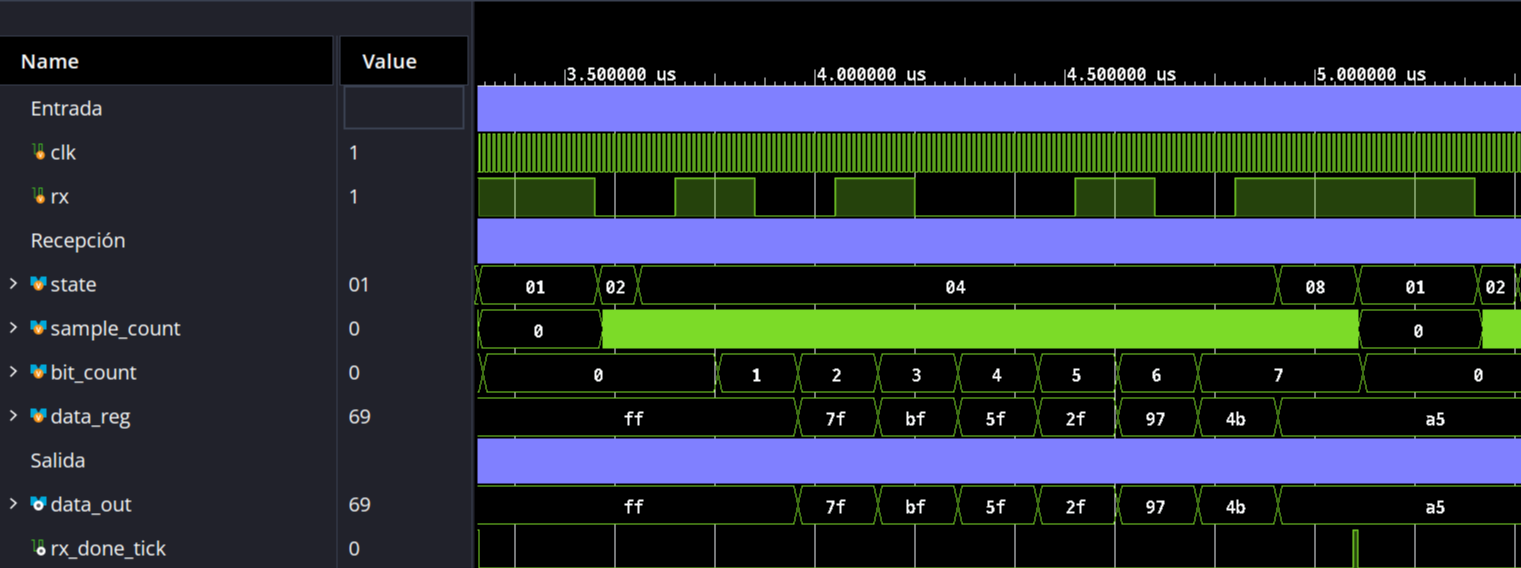
\includegraphics[width=\textwidth]{img/vivado_wave_uart_rx_a5.png}
  \caption{Recepción válida de \texttt{A5} en \texttt{uart\_rx\_tb}.}%
  \label{fig:wave-rx-a5}
\end{figure}

La figura~\ref{fig:wave-rx-errors} reúne las dos tramas defectuosas.
El pulso breve de la entrada produce el primer \texttt{frame\_error}.
La trama siguiente alcanza el estado DATA, pero el nivel bajo durante
el stop produce el segundo error. En ninguno de los casos se activa
\texttt{done}.

Después de detectar cada defecto, el estado RECOVER espera que la
entrada RX regrese al nivel alto antes de volver a IDLE. Por esta
razón, cada trama defectuosa genera un solo pulso de error.

\begin{figure}[H]
  \centering
  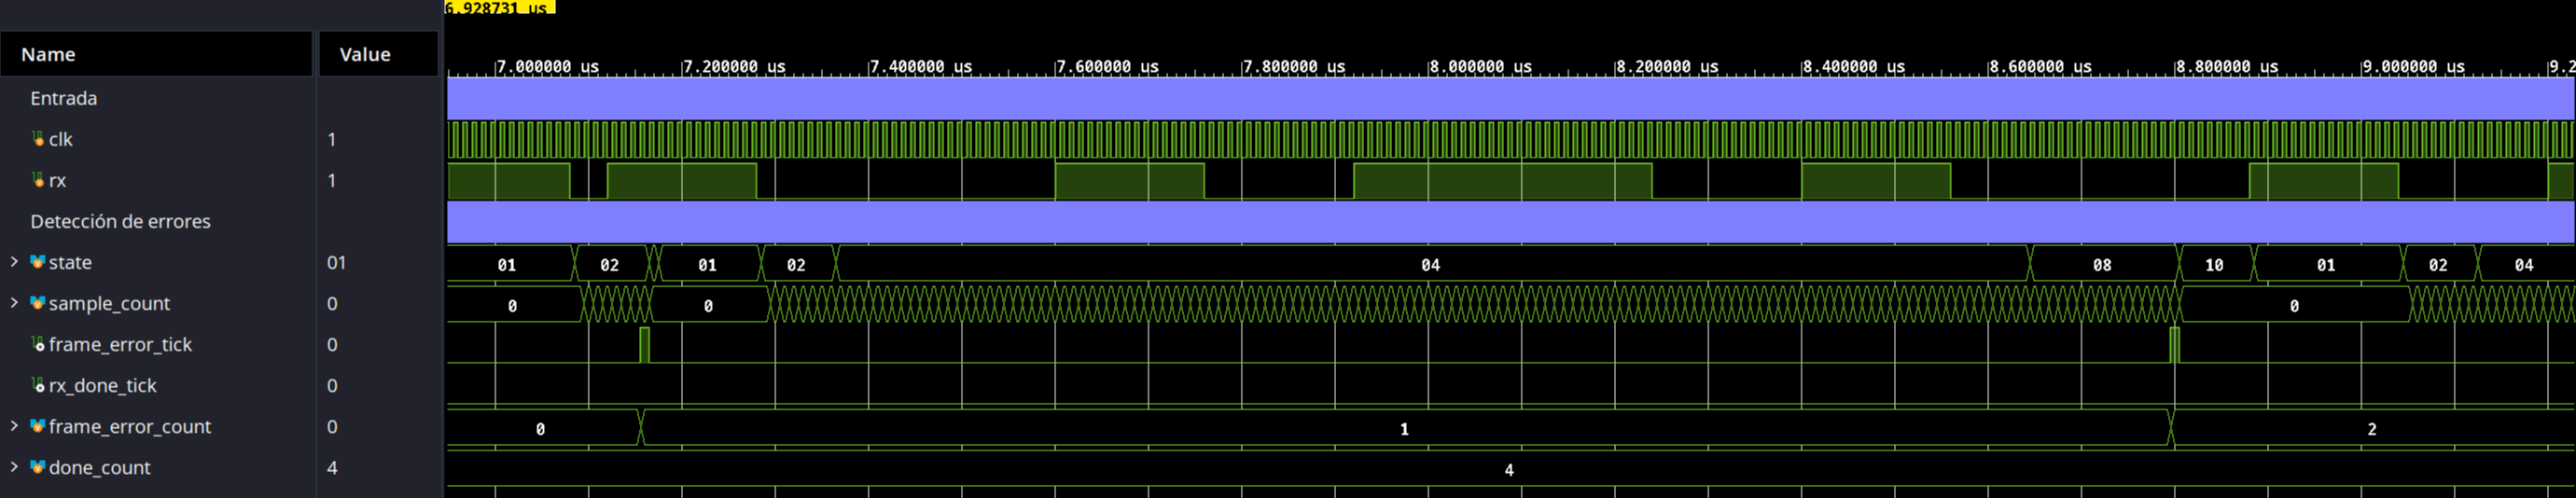
\includegraphics[width=\textwidth]{img/vivado_wave_uart_rx_errors.png}
  \caption{Detección de falso start y stop inválido en \texttt{uart\_rx\_tb}.}%
  \label{fig:wave-rx-errors}
\end{figure}

La figura~\ref{fig:wave-tx-a5} presenta la transmisión de \texttt{A5
= 1010\,0101}. Después del start en nivel bajo, la línea muestra la
secuencia 1, 0, 1, 0, 0, 1, 0, 1. Este orden corresponde al envío
desde D0 hasta D7. La señal \texttt{busy} permanece activa durante
toda la trama y \texttt{done} se mantiene en alto durante un solo
ciclo después del stop.

\begin{figure}[H]
  \centering
  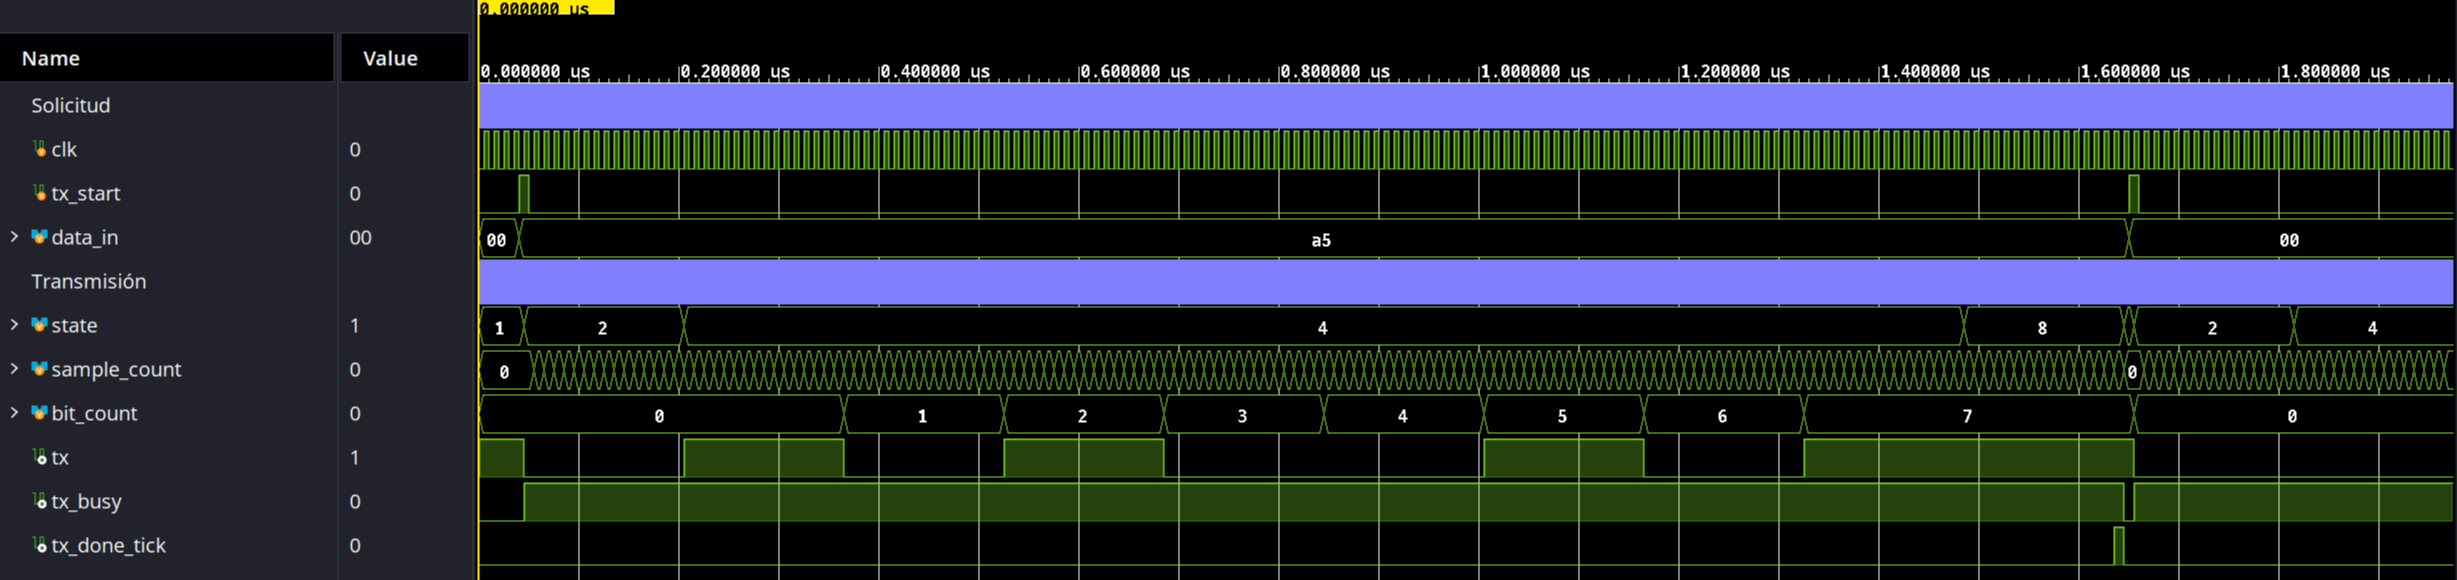
\includegraphics[width=\textwidth]{img/vivado_wave_uart_tx_a5.png}
  \caption{Serialización de \texttt{A5} en \texttt{uart\_tx\_tb}.}%
  \label{fig:wave-tx-a5}
\end{figure}

La figura~\ref{fig:wave-fifo} muestra la ocupación completa del FIFO.
El contador alcanza el valor cuatro y activa \texttt{full}. El
intento de escribir \texttt{99} no modifica el dato ubicado en la
cabeza de la cola.

Las escrituras posteriores reutilizan las posiciones liberadas, pero
no alteran el orden de lectura. La secuencia observada es
\texttt{11,22,33,44,55,66,77,88}. Al retirar el último dato, el
contador vuelve a cero y se activa \texttt{empty}.

\begin{figure}[H]
  \centering
  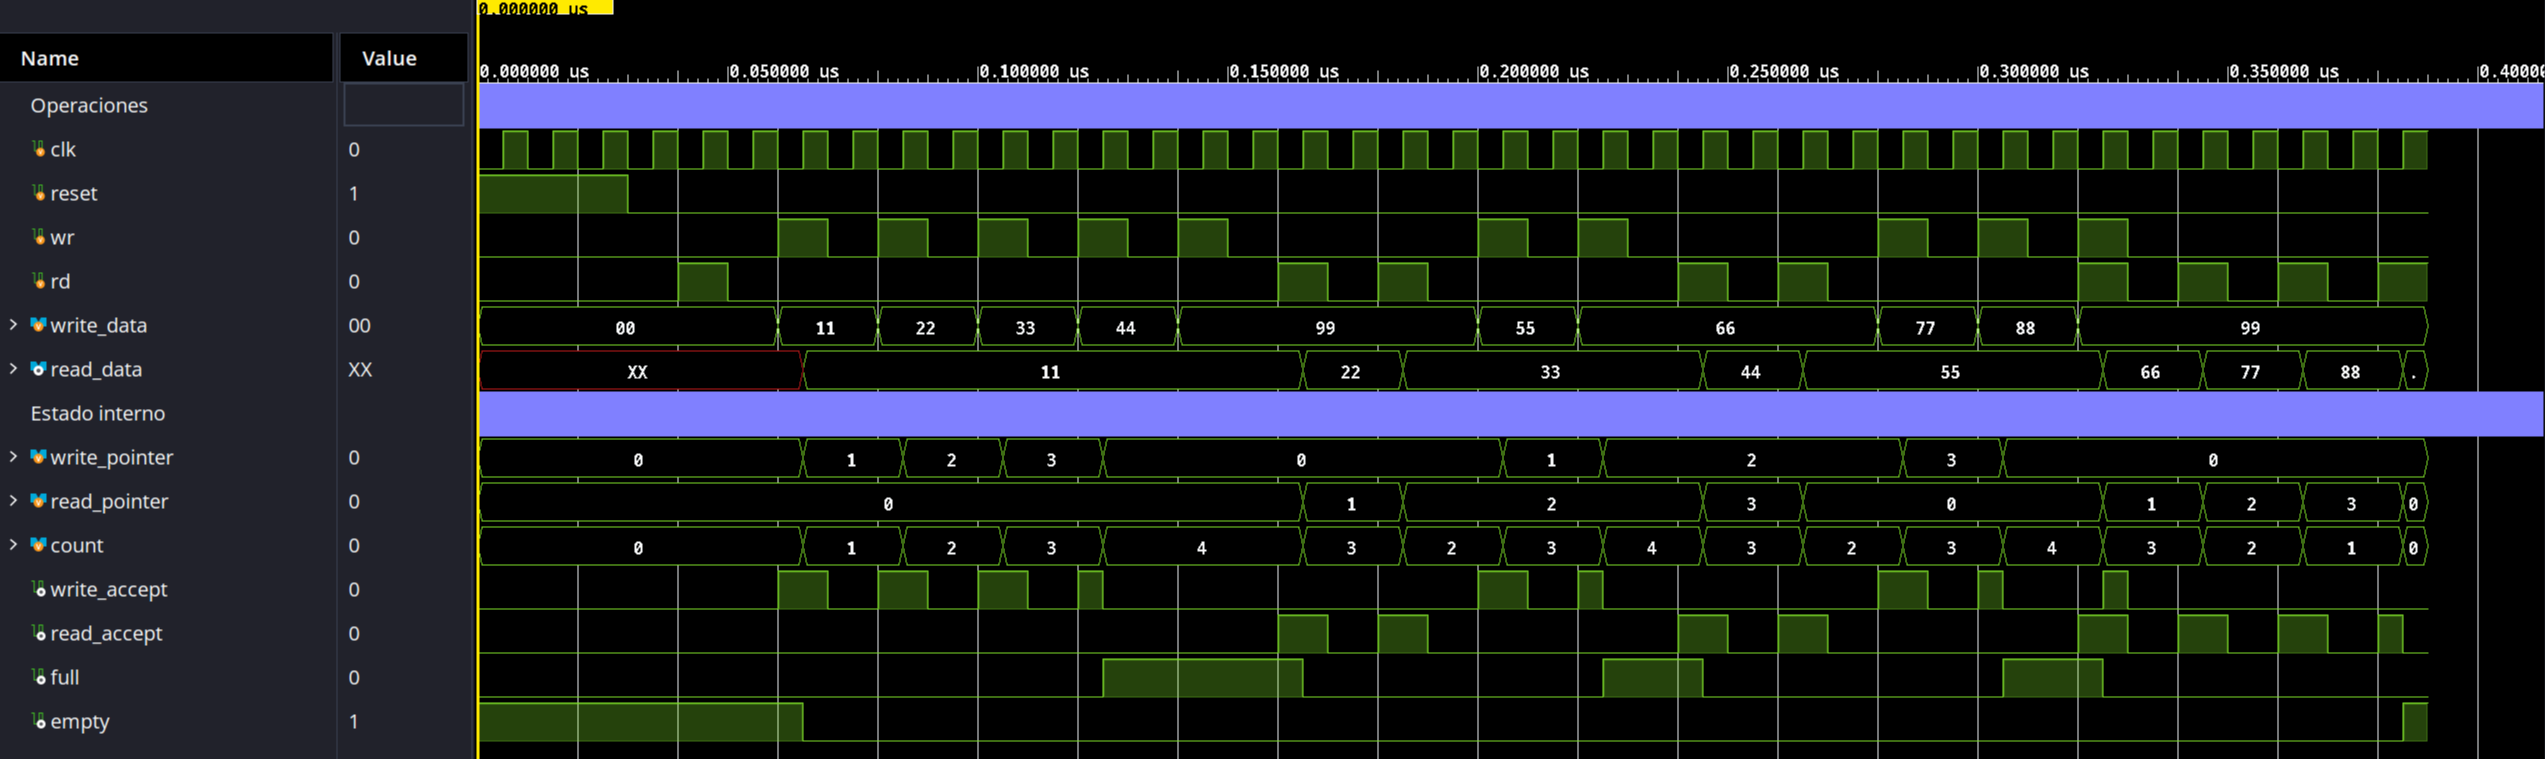
\includegraphics[width=\textwidth]{img/vivado_wave_fifo.png}
  \caption{Límites, accesos simultáneos y wrap-around en \texttt{fifo\_tb}.}%
  \label{fig:wave-fifo}
\end{figure}

\subsection{Interpretación}

Los cuatro bancos elementales finalizaron con el resultado PASS. Las
814 comparaciones de \texttt{alu\_tb.sv} confirmaron que la
integración no modificó el comportamiento de la ALU. La prueba de
\texttt{baud\_tick\_gen\_tb.sv} comprobó la periodicidad con la
parametrización reducida y utilizó la misma expresión del divisor que
el diseño. Este ensayo no mide la precisión del oscilador físico.

Las capturas del receptor y del transmisor muestran el recorrido
completo del byte \texttt{A5}. En ellas se puede seguir el orden de
los bits y el cambio de estado que ocurre durante cada parte de la
trama. Los demás bytes no se incluyeron en las figuras, pero fueron
comprobados automáticamente por sus respectivos bancos.

El archivo \texttt{fifo\_tb.sv} verificó que los datos se retiraran
en el mismo orden en que habían sido escritos. También comprobó que
\texttt{full} se activara al ocupar las cuatro posiciones y que
\texttt{empty} lo hiciera después de retirar el último dato.

Estas pruebas confirman el funcionamiento individual de los bloques.
Todavía no comprueban que el controlador pueda recibir una solicitud
completa ni que el resultado recorra todo el camino entre ambos pines UART.

\section{Subsistemas: núcleo UART y controlador}

Una vez verificados los bloques elementales, se probaron las dos
partes que coordinan el intercambio. El núcleo UART reúne el
receptor, el transmisor y las dos colas. El controlador interpreta
los bytes recibidos y genera la respuesta de la ALU. Los bancos de
este nivel permiten revisar esas funciones sin incorporar todavía el
recorrido completo por las líneas serie.

\subsection{Criterio y estímulos}

El archivo \texttt{tb/uart\_core\_tb.sv} verifica primero el camino
de recepción. Para ello envía cinco bytes consecutivos sobre RX sin
retirar ningún dato. Los primeros cuatro deben permanecer almacenados
en el FIFO. La llegada del quinto debe generar exactamente un
overrun. Después, el banco retira los cuatro bytes y comprueba que
mantengan el orden de llegada.

El mismo banco verifica luego el camino de transmisión. En este caso
escribe \texttt{A5}, \texttt{00}, \texttt{FF} y \texttt{3C} en la
cola correspondiente. Un decodificador implementado en el banco
reconstruye las cuatro tramas observadas sobre TX y compara los bytes obtenidos.

La prueba del controlador se encuentra en
\texttt{tb/alu\allowbreak\_uart\allowbreak\_controller\allowbreak\_tb.sv}.
Este banco entrega y retira bytes a través de la interfaz de los
FIFO. De este modo puede comprobar la interpretación de la secuencia
A--B--opcode sin incluir los tiempos propios de la transmisión UART.

Los casos dirigidos incluyen una suma normal, una suma con carry y
otra con overflow. También verifican SRA, AND, SUB, NOR, un opcode
inválido y un opcode con los bits superiores reservados. Para
comprobar la espera de la salida, el banco mantiene \texttt{tx\_full}
activo durante cinco ciclos. Por último, deja vencer el timeout de
una operación incompleta y aplica \texttt{rx\_error\_tick} después de
recibir el operando A.

\subsection{Resultado observado}

La figura~\ref{fig:wave-controller} permite seguir primero la
operación \texttt{7F 01 20}. En la parte superior aparecen los tres
bytes de la solicitud sobre \texttt{r\_data}. Cada vez que hay un
byte disponible, el controlador activa \texttt{rd\_uart} para
retirarlo de la cola de recepción. Las tres lecturas almacenan el
operando A, el operando B y el opcode. Al mismo tiempo, el estado
avanza por WAIT\_A, WAIT\_B y WAIT\_OPCODE.

Después de recibir el opcode, el controlador pasa a EXECUTE. El pulso
\texttt{capture\_result} registra el resultado \texttt{80} y las
banderas de la ALU. En ese momento, \texttt{result\_reg} toma el
valor \texttt{80} y los LED cambian a \texttt{480}. Los tres bits
superiores de este patrón indican que la bandera V está activa. Como
la cola de transmisión tiene espacio, \texttt{w\_data} presenta el
resultado y \texttt{wr\_uart} genera el pulso que lo escribe en el FIFO.

La parte derecha de la captura muestra una situación diferente con la
operación \texttt{0C 0A 24}. El controlador recibe los tres bytes y
calcula el resultado \texttt{C0}, pero \texttt{tx\_full} se encuentra
en alto. Por esta razón, permanece en WAIT\_TX y conserva la
respuesta en \texttt{result\_reg}. Durante esa espera,
\texttt{wr\_uart} permanece en bajo y el resultado no se escribe en
una cola que ya está llena.

Cuando \texttt{tx\_full} vuelve a cero, el controlador genera el
pulso de escritura y entrega la respuesta pendiente. Recién entonces
regresa a WAIT\_A para comenzar una nueva solicitud. Esta parte de la
figura muestra que una demora en la transmisión no provoca la pérdida
del resultado calculado.

\begin{figure}[H]
  \centering
  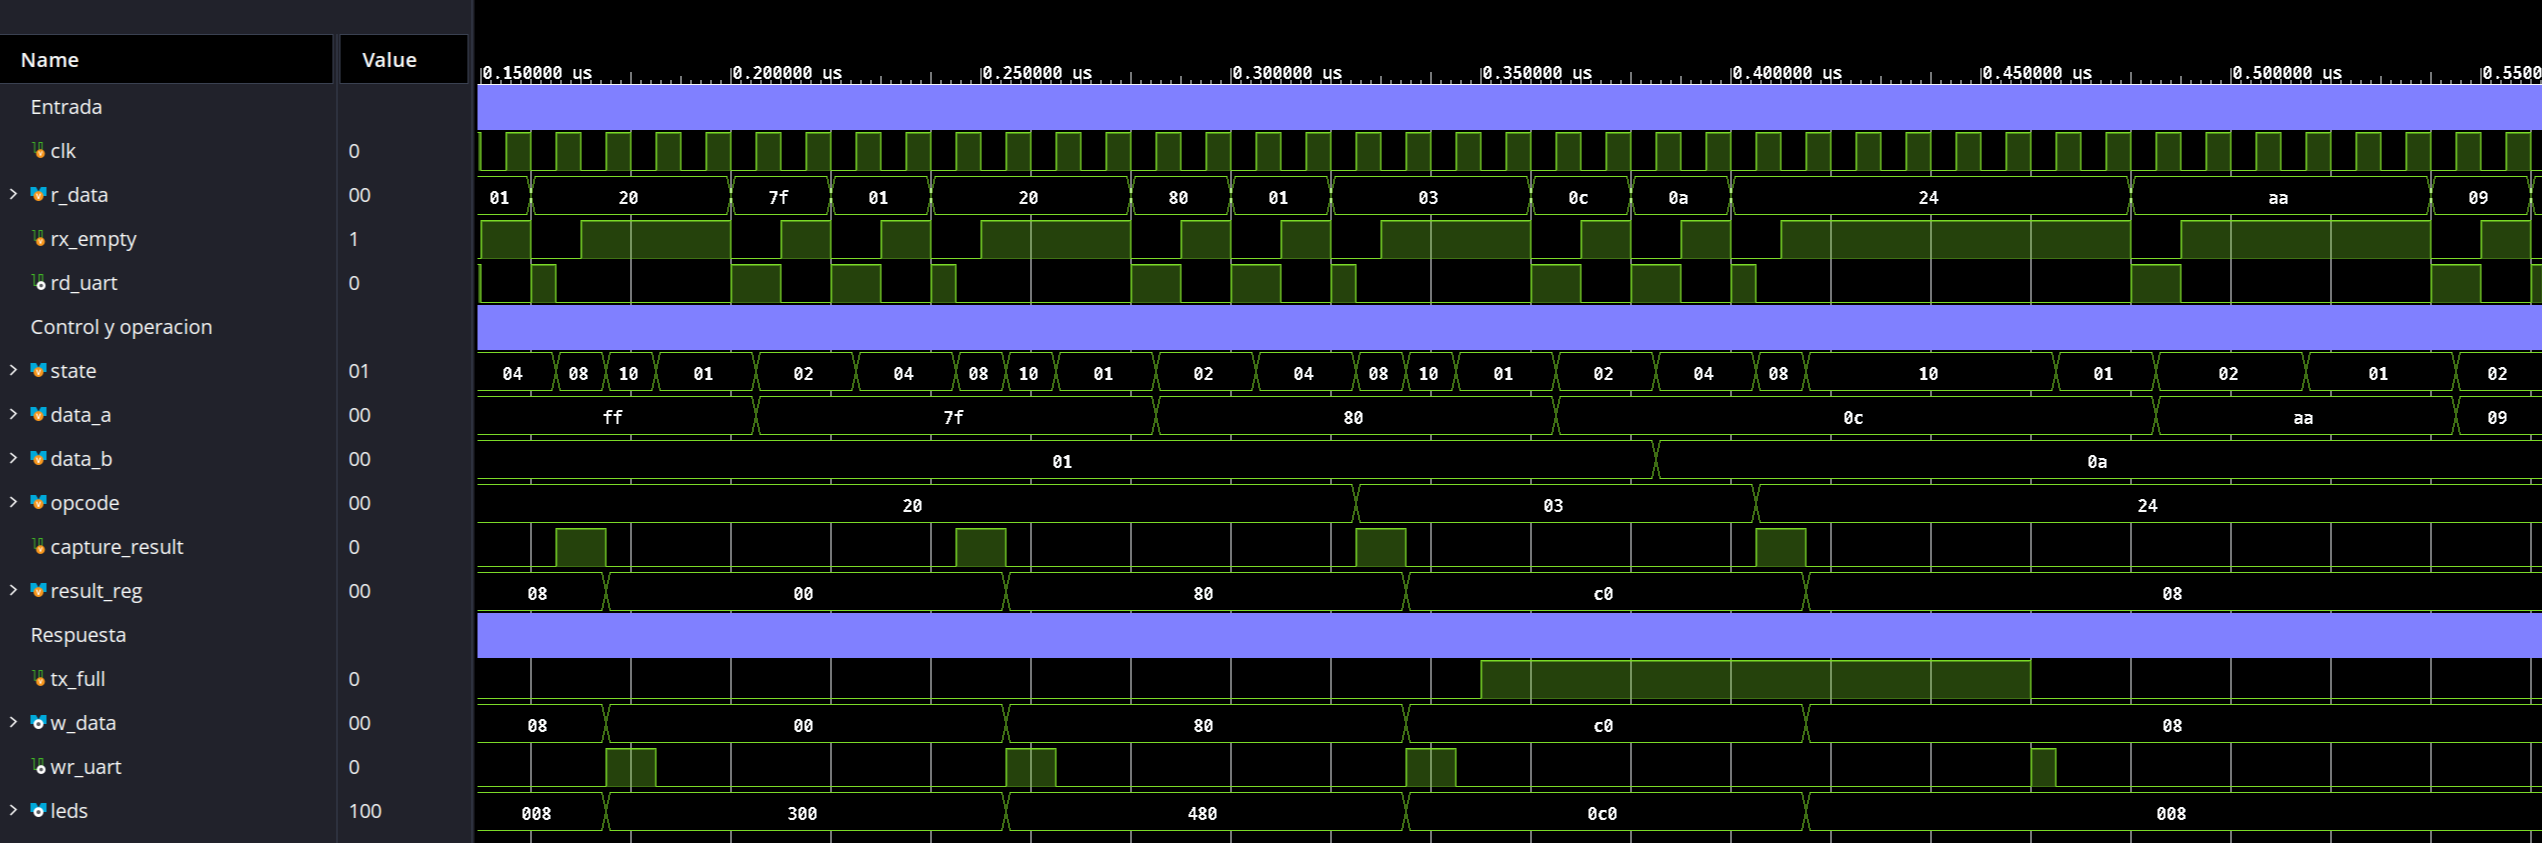
\includegraphics[width=\textwidth]{img/vivado_wave_controller.png}
  \caption{Operación y espera por capacidad en
  \texttt{alu\_uart\_controller\_tb}.}%
  \label{fig:wave-controller}
\end{figure}

XSim informó \texttt{PASS: UART core FIFOs, overrun and serialized
output} al finalizar el banco del núcleo. Para el controlador informó
\texttt{PASS: ALU/UART controller protocol, stalls and recovery}.
Ninguno de los bancos produjo errores fatales ni alcanzó el límite de
su watchdog.

\subsection{Interpretación}

El banco del núcleo confirmó que las colas conservan el orden de los
bytes. La prueba de recepción completa mostró además que un dato
adicional produce un error de overrun en lugar de sobrescribir el
elemento más antiguo.

El banco del controlador confirmó que una respuesta permanece
registrada mientras la cola de transmisión está llena. También
verificó que EXECUTE separa la captura del opcode del registro del
resultado. Los casos de timeout y error de recepción mostraron que
una solicitud incompleta se descarta antes de aceptar una nueva.

En estas pruebas, uno de los extremos todavía es reemplazado por el
propio banco. El núcleo UART no está conectado a la ALU y el
controlador recibe bytes completos sin atravesar el receptor. Por lo
tanto, los resultados de este nivel no sustituyen una prueba del
sistema integrado.

\section{Verificación extremo a extremo}

El último nivel comprueba el funcionamiento del módulo superior. En
esta prueba los estímulos ingresan como bits por \texttt{serial\_rx}.
La respuesta también se observa como una trama completa sobre
\texttt{serial\_tx}. De esta manera se incluye el mismo recorrido que
utiliza una operación dentro de la FPGA.

\subsection{Criterio y estímulos}

El archivo \texttt{tb/alu\_uart\_top\_tb.sv} instancia el
sincronizador, el generador de ticks, el receptor, el transmisor, los
dos FIFO, el controlador y la ALU. Para conservar las relaciones
temporales y reducir el costo de la simulación, utiliza un reloj de
\SI{100}{\kilo\hertz}, una velocidad de \num{2500} baud y un
sobremuestreo 4x. Con estos parámetros, el divisor permanece en diez
y cada bit dura cuarenta ciclos.

El banco no fuerza ninguna señal interna. Los estímulos modifican
únicamente \texttt{serial\_rx} y la respuesta se reconstruye a partir
de \texttt{serial\_tx}.

Los primeros doce casos son dirigidos. En las operaciones válidas se
incluyen una suma normal, una suma con carry, una suma con overflow,
SUB, SRA, SRL y NOR. También se comprueban un opcode inválido y un
opcode con los bits superiores reservados.

Los tres casos restantes se concentran en la recuperación. El primero
envía un byte aislado y espera que venza el timeout. El segundo
introduce un bit de stop inválido y luego transmite una operación
correcta. El tercero activa el reset durante una trama.

Después de los casos dirigidos, el banco aplica cien pares
pseudoaleatorios para cada una de las ocho operaciones. La secuencia
utiliza la semilla \texttt{32'h1a2b3c4d}. En total se ejecutan 800
operaciones aleatorias y 812 transacciones.

\subsection{Resultado observado}

La figura~\ref{fig:wave-top-end-to-end} muestra la primera operación,
representada por los bytes \texttt{05 03 20}. Sobre RX se distinguen
tres grupos de diez bits. Cada pulso \texttt{rx\_done} publica uno de
los bytes y hace avanzar al controlador.

Después de recibir el opcode se activa \texttt{enqueue}. La cola de
transmisión recibe \texttt{08} y \texttt{serial\_tx} comienza a
emitir la trama de respuesta. Antes de completar la operación, los
LED muestran \texttt{100}. Este valor corresponde al resultado cero
con la bandera Z activa. Luego cambian a \texttt{008}, que representa
el resultado ocho sin banderas activas.

\begin{figure}[H]
  \centering
  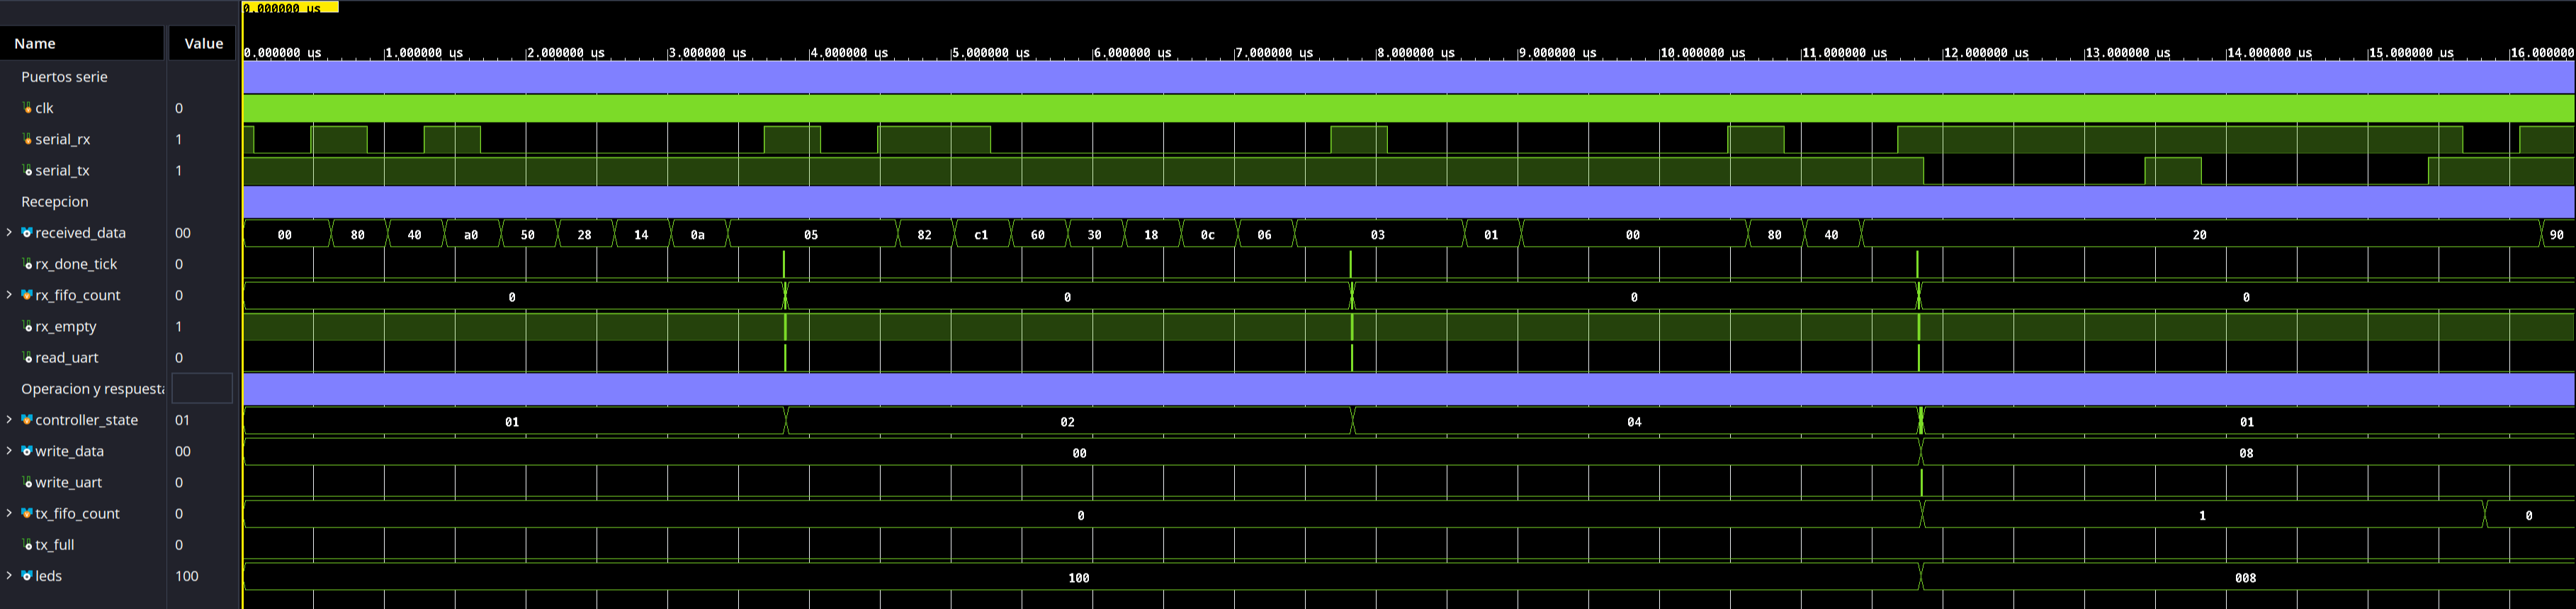
\includegraphics[width=\textwidth]{img/vivado_wave_top_end_to_end.png}
  \caption{Recorrido completo de \texttt{05 03 20} en
  \texttt{alu\_uart\_top\_tb}.}%
  \label{fig:wave-top-end-to-end}
\end{figure}

La regresión completa se compiló y ejecutó nuevamente mediante el
archivo \texttt{scripts/run\allowbreak\_tests.sh} con XSim 2025.2. La
figura~\ref{fig:regresion-xsim} reúne las líneas finales emitidas por
los ocho bancos. El registro completo de la ejecución se conserva en
\texttt{reports/simulation\allowbreak\_regression.log}.

El banco superior finalizó con \texttt{PASS: 812 complete serial ALU
transactions}. Después de ejecutar los ocho bancos, el script informó
\texttt{PASS: 8 testbenches completados}.

\begin{figure}[H]
  \centering
  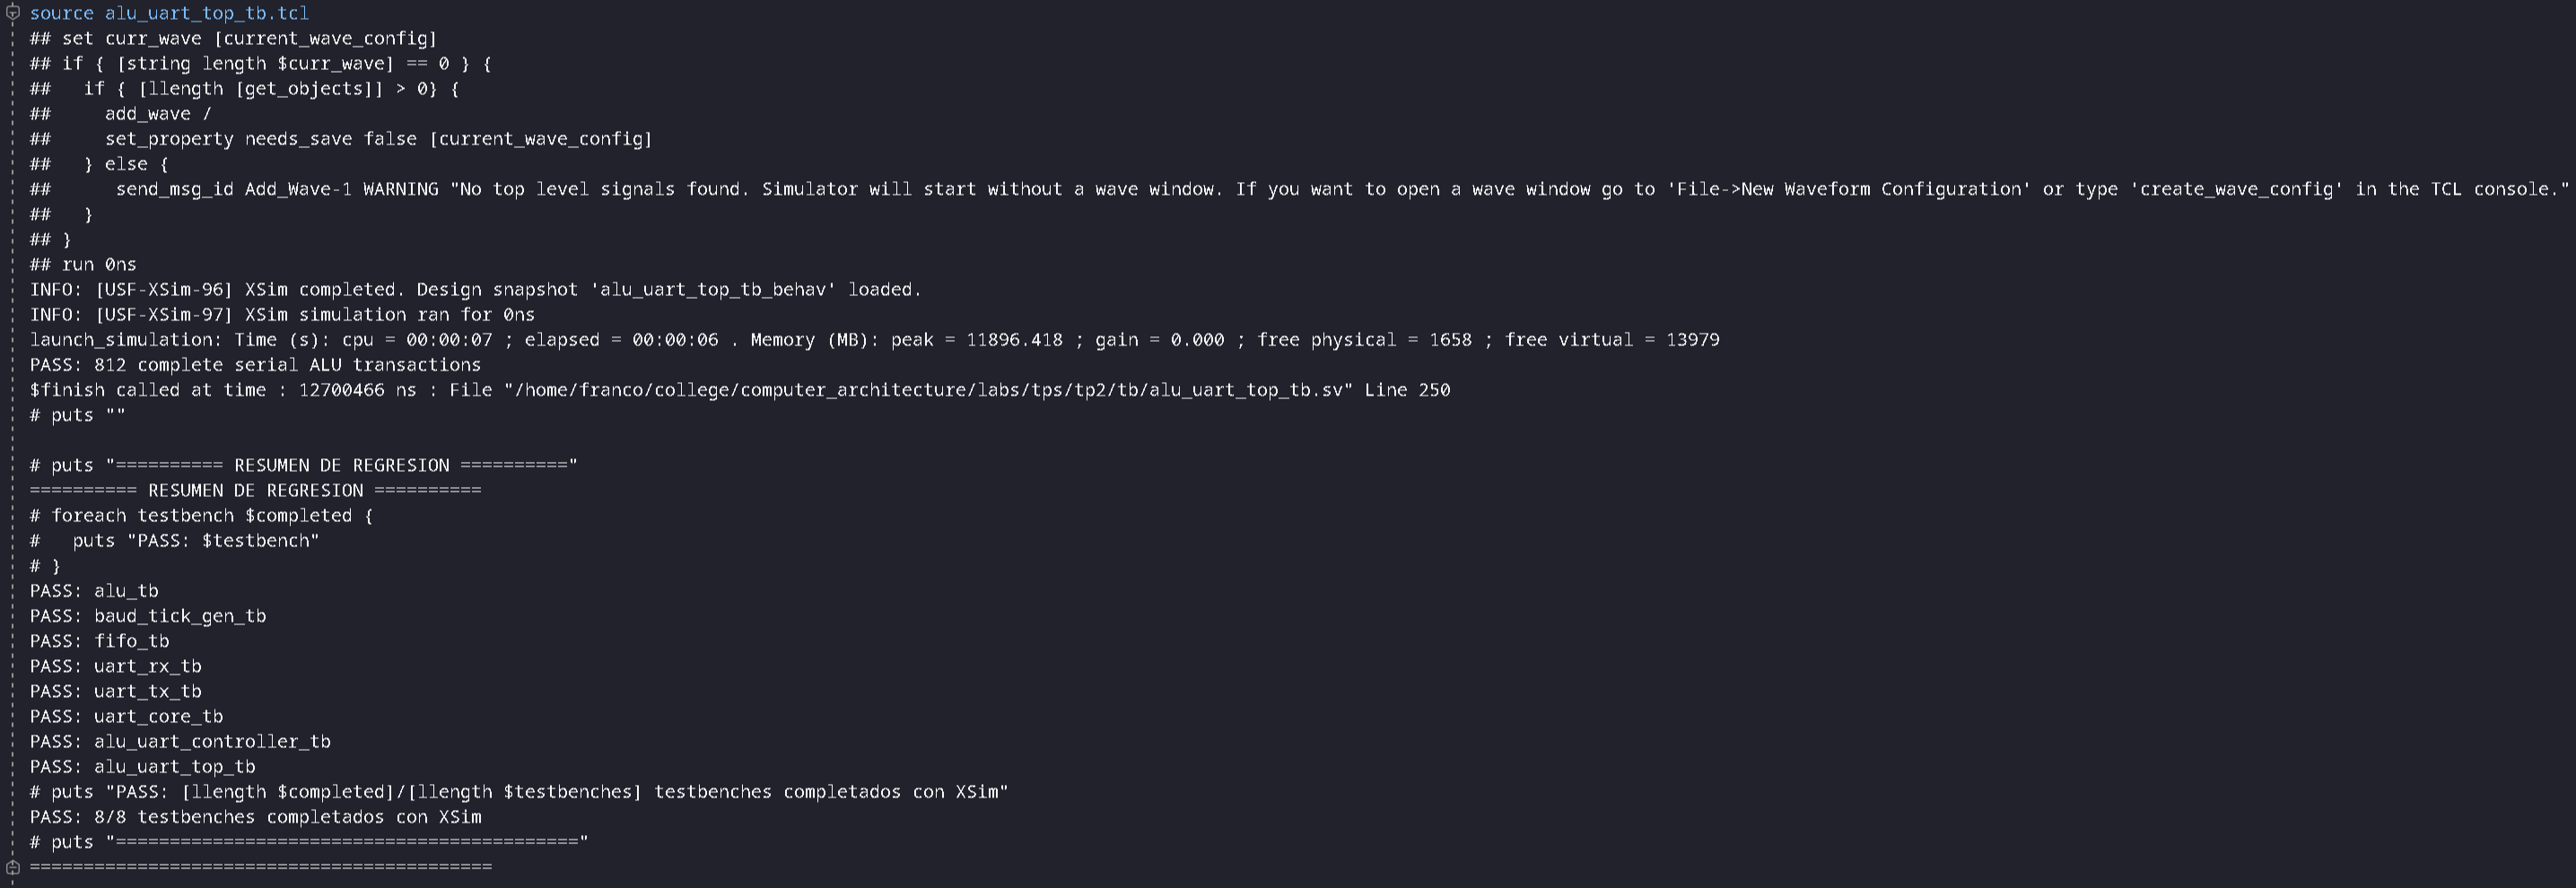
\includegraphics[width=\textwidth]{img/vivado_simulation_regression.png}
  \caption{Resultado de la regresión completa ejecutada con XSim 2025.2.}%
  \label{fig:regresion-xsim}
\end{figure}

\begin{table}[H]
  \centering
  \begin{tabularx}{\textwidth}{L{5.1cm}C{2.2cm}Y}
    \toprule
    \textbf{Banco} & \textbf{Estado} & \textbf{Resultado principal} \\
    \midrule
    \texttt{alu\_tb} & PASS & 814 comprobaciones. \\
    \texttt{baud\_tick\_gen\_tb} & PASS & Tick cada diez ciclos. \\
    \texttt{fifo\_tb} & PASS & Fronteras y wrap-around. \\
    \texttt{uart\_rx\_tb} & PASS & Tramas válidas y defectuosas. \\
    \texttt{uart\_tx\_tb} & PASS & Framing, orden y tiempos. \\
    \texttt{uart\_core\_tb} & PASS & FIFO, overrun y salida serie. \\
    \texttt{alu\_uart\_controller\_tb} & PASS & Protocolo y recuperación. \\
    \texttt{alu\_uart\_top\_tb} & PASS & 812 transacciones completas. \\
    \bottomrule
  \end{tabularx}
  \caption{Resultado de la regresión RTL completa.}%
\end{table}

\subsection{Interpretación}

El banco superior comprobó el recorrido funcional desde el pin RX
hasta el pin TX. La prueba incluyó el orden de los bits, el
almacenamiento de los bytes, la ejecución de la ALU, la transmisión
de la respuesta y la permanencia del resultado en los LED.

Los casos de recuperación confirmaron que el timeout, el bit de stop
inválido y el reset no producen una respuesta espuria. Después de
cada situación, una transacción nueva pudo completarse correctamente.
Las 800 operaciones aleatorias ampliaron la cantidad de operandos
ejercitados mediante una secuencia que puede repetirse con la misma semilla.

Estos resultados comprueban el comportamiento funcional del RTL, pero
no representan todos los fenómenos presentes en el circuito físico.
La simulación no modela la metastabilidad analógica ni el ruido de
las señales. Tampoco incluye la tolerancia de los osciladores, las
demoras del enlace USB ni los retardos obtenidos después del ruteo.

El análisis CDC y la verificación temporal del diseño implementado
consideran parte de estos aspectos en las secciones siguientes. La
comunicación con el puente USB--UART y la observación de los LED
requieren una comprobación posterior sobre la placa.


\chapter{Síntesis e implementación}
\section{Flujo sobre el dispositivo objetivo}

La simulación funcional permite comprobar el comportamiento del RTL,
pero no muestra cómo se utiliza el dispositivo físico. Para obtener
esa información, el diseño se sintetizó y se implementó sobre la FPGA
Artix-7 \texttt{xc7a35tcpg236-1} de la Basys 3.

Durante la síntesis, Vivado interpreta los módulos SystemVerilog y
los traduce a una red formada por registros, memorias, operadores y
máquinas de estado. La implementación toma esa red y asigna cada
recurso a una ubicación concreta del dispositivo. En esta etapa
también realiza la colocación, el ruteo y el cálculo de los retardos
físicos. Una vez completadas ambas etapas, se genera el bitstream
utilizado para programar la placa.

El proceso se automatizó mediante dos archivos. El script
\texttt{scripts/create\_project.tcl} crea el proyecto para el
dispositivo seleccionado. También agrega las diez fuentes RTL, los
ocho bancos de pruebas y el archivo de restricciones
\texttt{basys3.xdc}. Finalmente, establece \texttt{alu\_uart\_top}
como módulo superior.

El script \texttt{scripts/build\_bitstream.tcl} ejecuta la
construcción del diseño. Primero reinicia las corridas anteriores y
vuelve a realizar la síntesis y la implementación. Luego guarda en el
directorio \texttt{reports/} los reportes de utilización,
metodología, temporización, CDC y DRC. El mismo script genera el
archivo \texttt{build/alu\_uart\_top.bit}.

La creación del proyecto y la construcción completa pueden repetirse
con los siguientes comandos:

% tex-fmt: off
\begin{codebox}
vivado -mode batch -source scripts/create_project.tcl
vivado -mode batch -source scripts/build_bitstream.tcl
\end{codebox}
% tex-fmt: on

La construcción utilizada para este informe se realizó con Vivado
2025.2, build 6299465. La síntesis terminó sin errores, advertencias
críticas ni advertencias. Durante la implementación, el ruteo
finalizó con el mensaje \texttt{Router Completed Successfully}. La
figura~\ref{fig:corridas-vivado} muestra el estado final de ambas corridas.

\begin{figure}[H]
  \centering
  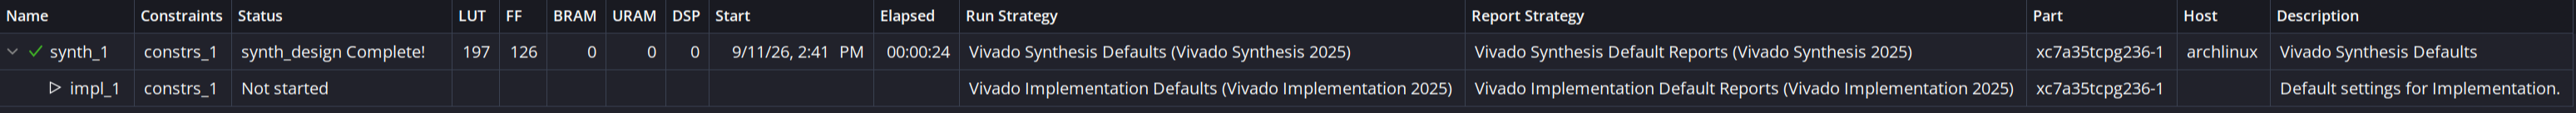
\includegraphics[width=\textwidth,trim=0 0 2347 0,clip]
  {img/vivado_synthesis_successful.png}
  \vspace{0.5em}

  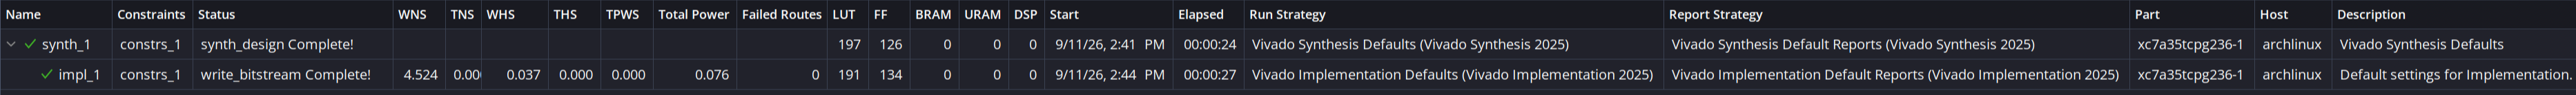
\includegraphics[width=\textwidth,trim=0 0 2500 0,clip]
  {img/vivado_implementation_successful.png}
  \caption{Corridas de síntesis e implementación completadas en Vivado.}%
  \label{fig:corridas-vivado}
\end{figure}

El bitstream obtenido corresponde al dispositivo declarado y ocupa
326538 bytes. La figura~\ref{fig:flujo-vivado} resume el recorrido
desde las fuentes SystemVerilog hasta ese archivo. Los resultados de
utilización, temporización, CDC y DRC se producen durante las etapas
intermedias y se analizan por separado en las secciones siguientes.

\begin{figure}[H]
  \centering
  \begin{tikzpicture}[
      stage/.style={draw=coderule,fill=codeback,rounded corners=2mm,
      minimum width=3.0cm,minimum height=1.35cm,align=center,thick},
      ok/.style={font=\small\bfseries,text=technicalviolet},
      arrow/.style={-{Latex[length=2.4mm]},thick,draw=codeviolet}
    ]
    \node[stage] at (0,0) (rtl) {SystemVerilog\\10 módulos};
    \node[stage] at (4.1,0) (synth) {Síntesis\\0 errores};
    \node[stage] at (8.2,0) (place) {Place \& route\\completado};
    \node[stage] at (12.3,0) (bit) {Bitstream\\326538 bytes};
    \draw[arrow] (rtl) -- (synth);
    \draw[arrow] (synth) -- (place);
    \draw[arrow] (place) -- (bit);
    \node[ok,below=0.3cm of synth] {FSM y LUTRAM extraídas};
    \node[ok,below=0.3cm of place] {timing, CDC y DRC};
  \end{tikzpicture}
  \caption{Recorrido reproducido desde RTL hasta el bitstream.}%
  \label{fig:flujo-vivado}
\end{figure}

\section{Elaboración y comprobación del RTL}

Antes de traducir el diseño a los recursos de la FPGA, Vivado elabora
las fuentes y construye su jerarquía lógica. Esta etapa permite
comprobar que los módulos, las instancias y sus conexiones fueron
interpretados de acuerdo con la descripción SystemVerilog.

La figura~\ref{fig:sources-vivado} muestra las fuentes incorporadas
al proyecto. Allí se reconoce el archivo
\texttt{rtl/alu\allowbreak\_uart\allowbreak\_top.sv} como nivel
superior, junto con sus instancias sintetizables. También aparecen
\texttt{basys3.xdc} y los ocho bancos utilizados durante la simulación.

\begin{figure}[H]
  \centering
  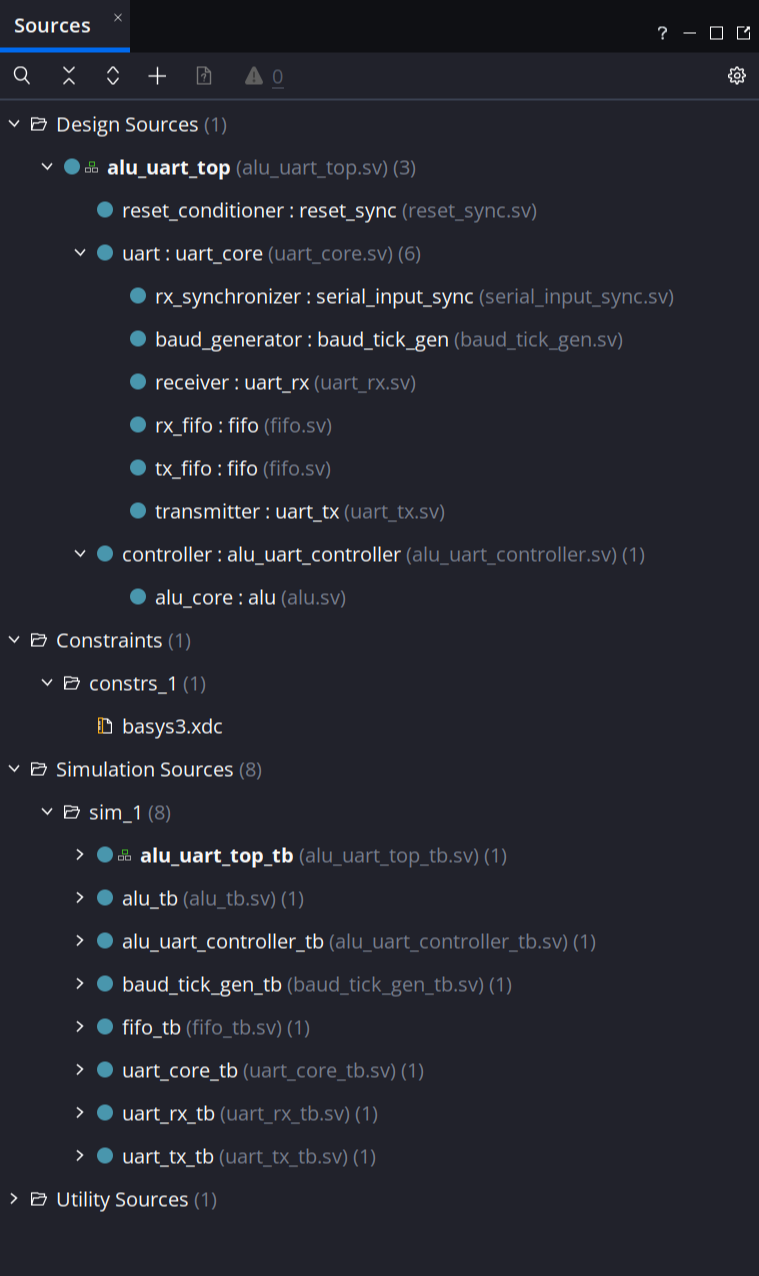
\includegraphics[height=14.2cm,keepaspectratio]{img/vivado_sources.png}
  \caption{Jerarquía de fuentes, restricciones y bancos de pruebas en Vivado.}%
  \label{fig:sources-vivado}
\end{figure}

Sobre esta misma configuración se ejecutó el análisis estático del
RTL. La herramienta revisó la descripción antes de la síntesis y no
encontró violaciones. El resultado se observa en la
figura~\ref{fig:linter-vivado}.

\begin{figure}[H]
  \centering
  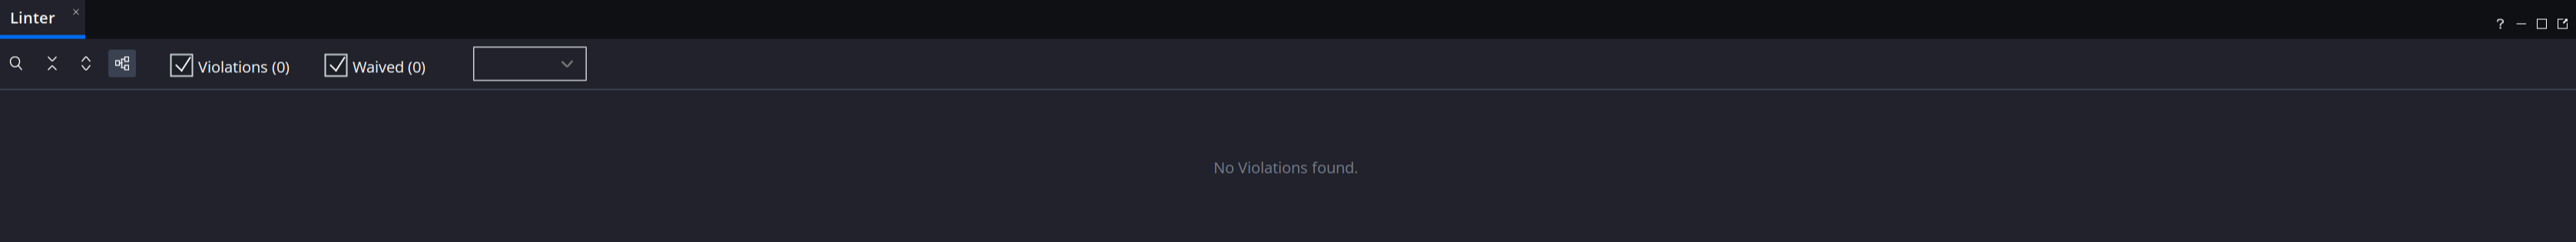
\includegraphics[width=\textwidth]{img/vivado_linter.png}
  \caption{Análisis estático del RTL sin violaciones.}%
  \label{fig:linter-vivado}
\end{figure}

Los esquemáticos elaborados permiten revisar la estructura que Vivado
obtuvo a partir de las fuentes. En esta vista todavía se conservan
los módulos del RTL. Por lo tanto, resulta posible comparar
directamente la jerarquía generada con la arquitectura presentada anteriormente.

La revisión comienza en el nivel superior. En la
figura~\ref{fig:schematic-top-rtl} se distinguen el acondicionador
del reset, el núcleo UART y el controlador de las transacciones.
Estos bloques se mantienen separados y se conectan mediante las
señales definidas en \texttt{rtl/alu\_uart\_top.sv}.

\begin{figure}[H]
  \centering
  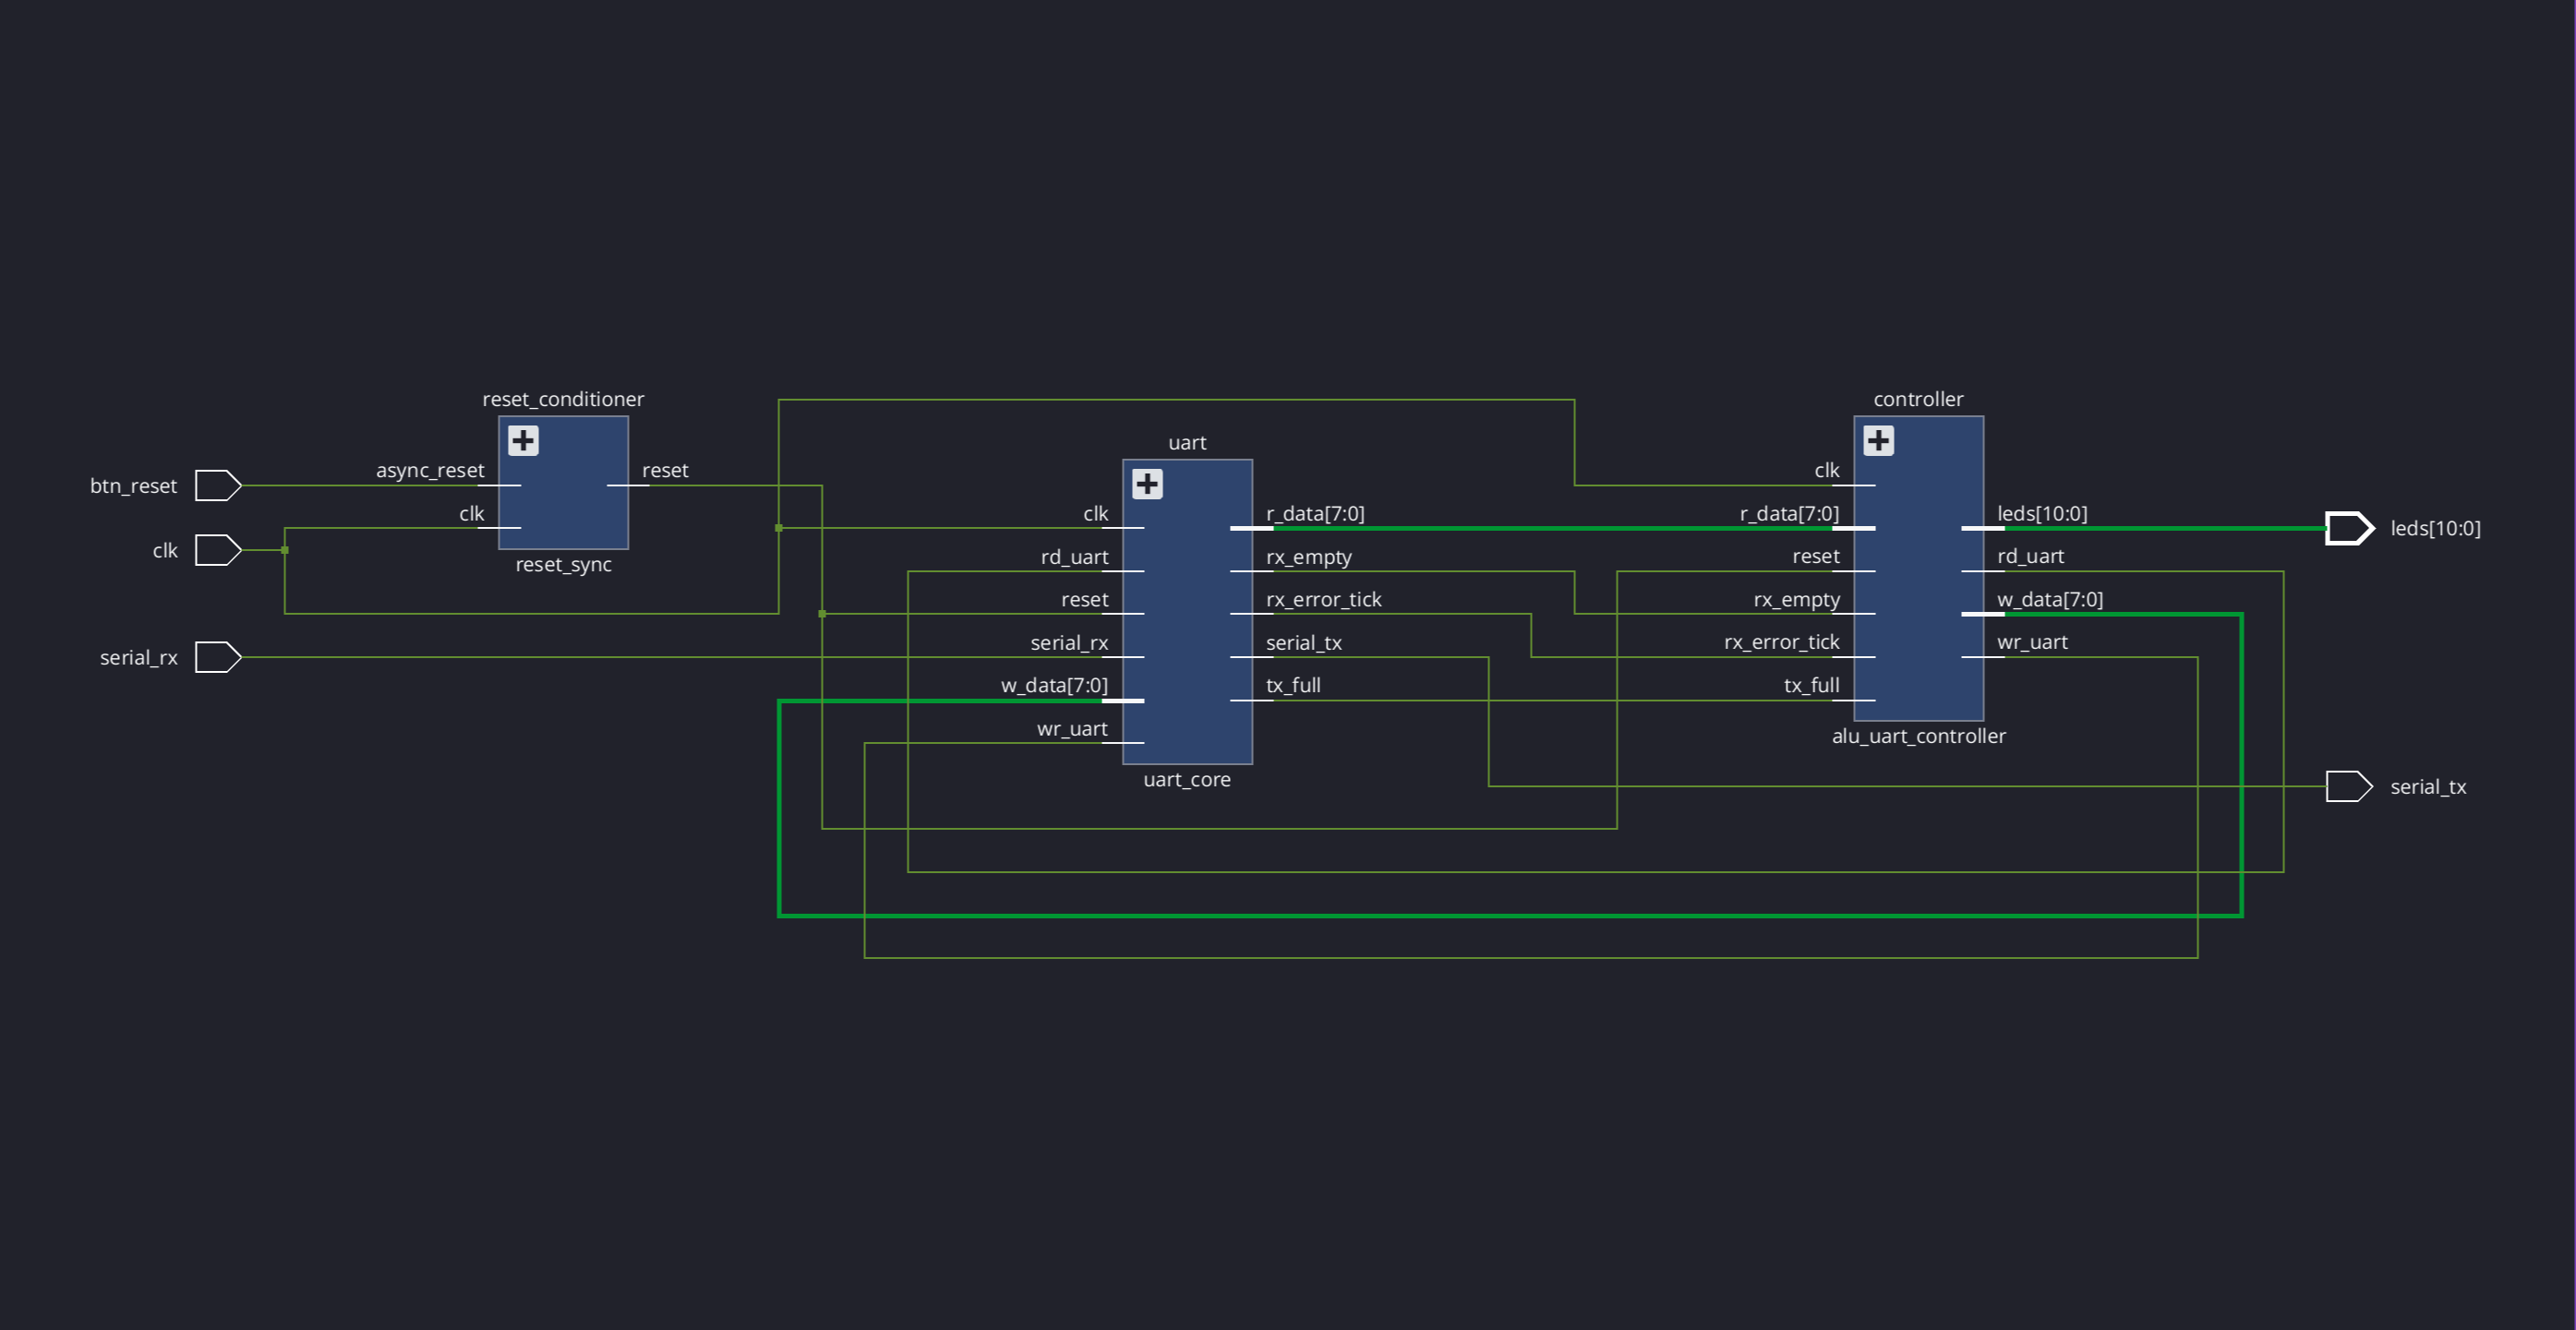
\includegraphics[width=0.92\textwidth]{img/vivado_schematic_top_rtl.png}
  \caption{Esquemático RTL elaborado de \texttt{alu\_uart\_top}.}%
  \label{fig:schematic-top-rtl}
\end{figure}

Al ingresar en el núcleo UART se observan los dos caminos de la
comunicación. La figura~\ref{fig:schematic-uart-core-rtl} muestra el
receptor con su FIFO y el transmisor con la cola de salida. Ambos
caminos utilizan el mismo generador de muestreo. Esta organización
coincide con la descripción del archivo \texttt{rtl/uart\_core.sv}.

\begin{figure}[H]
  \centering
  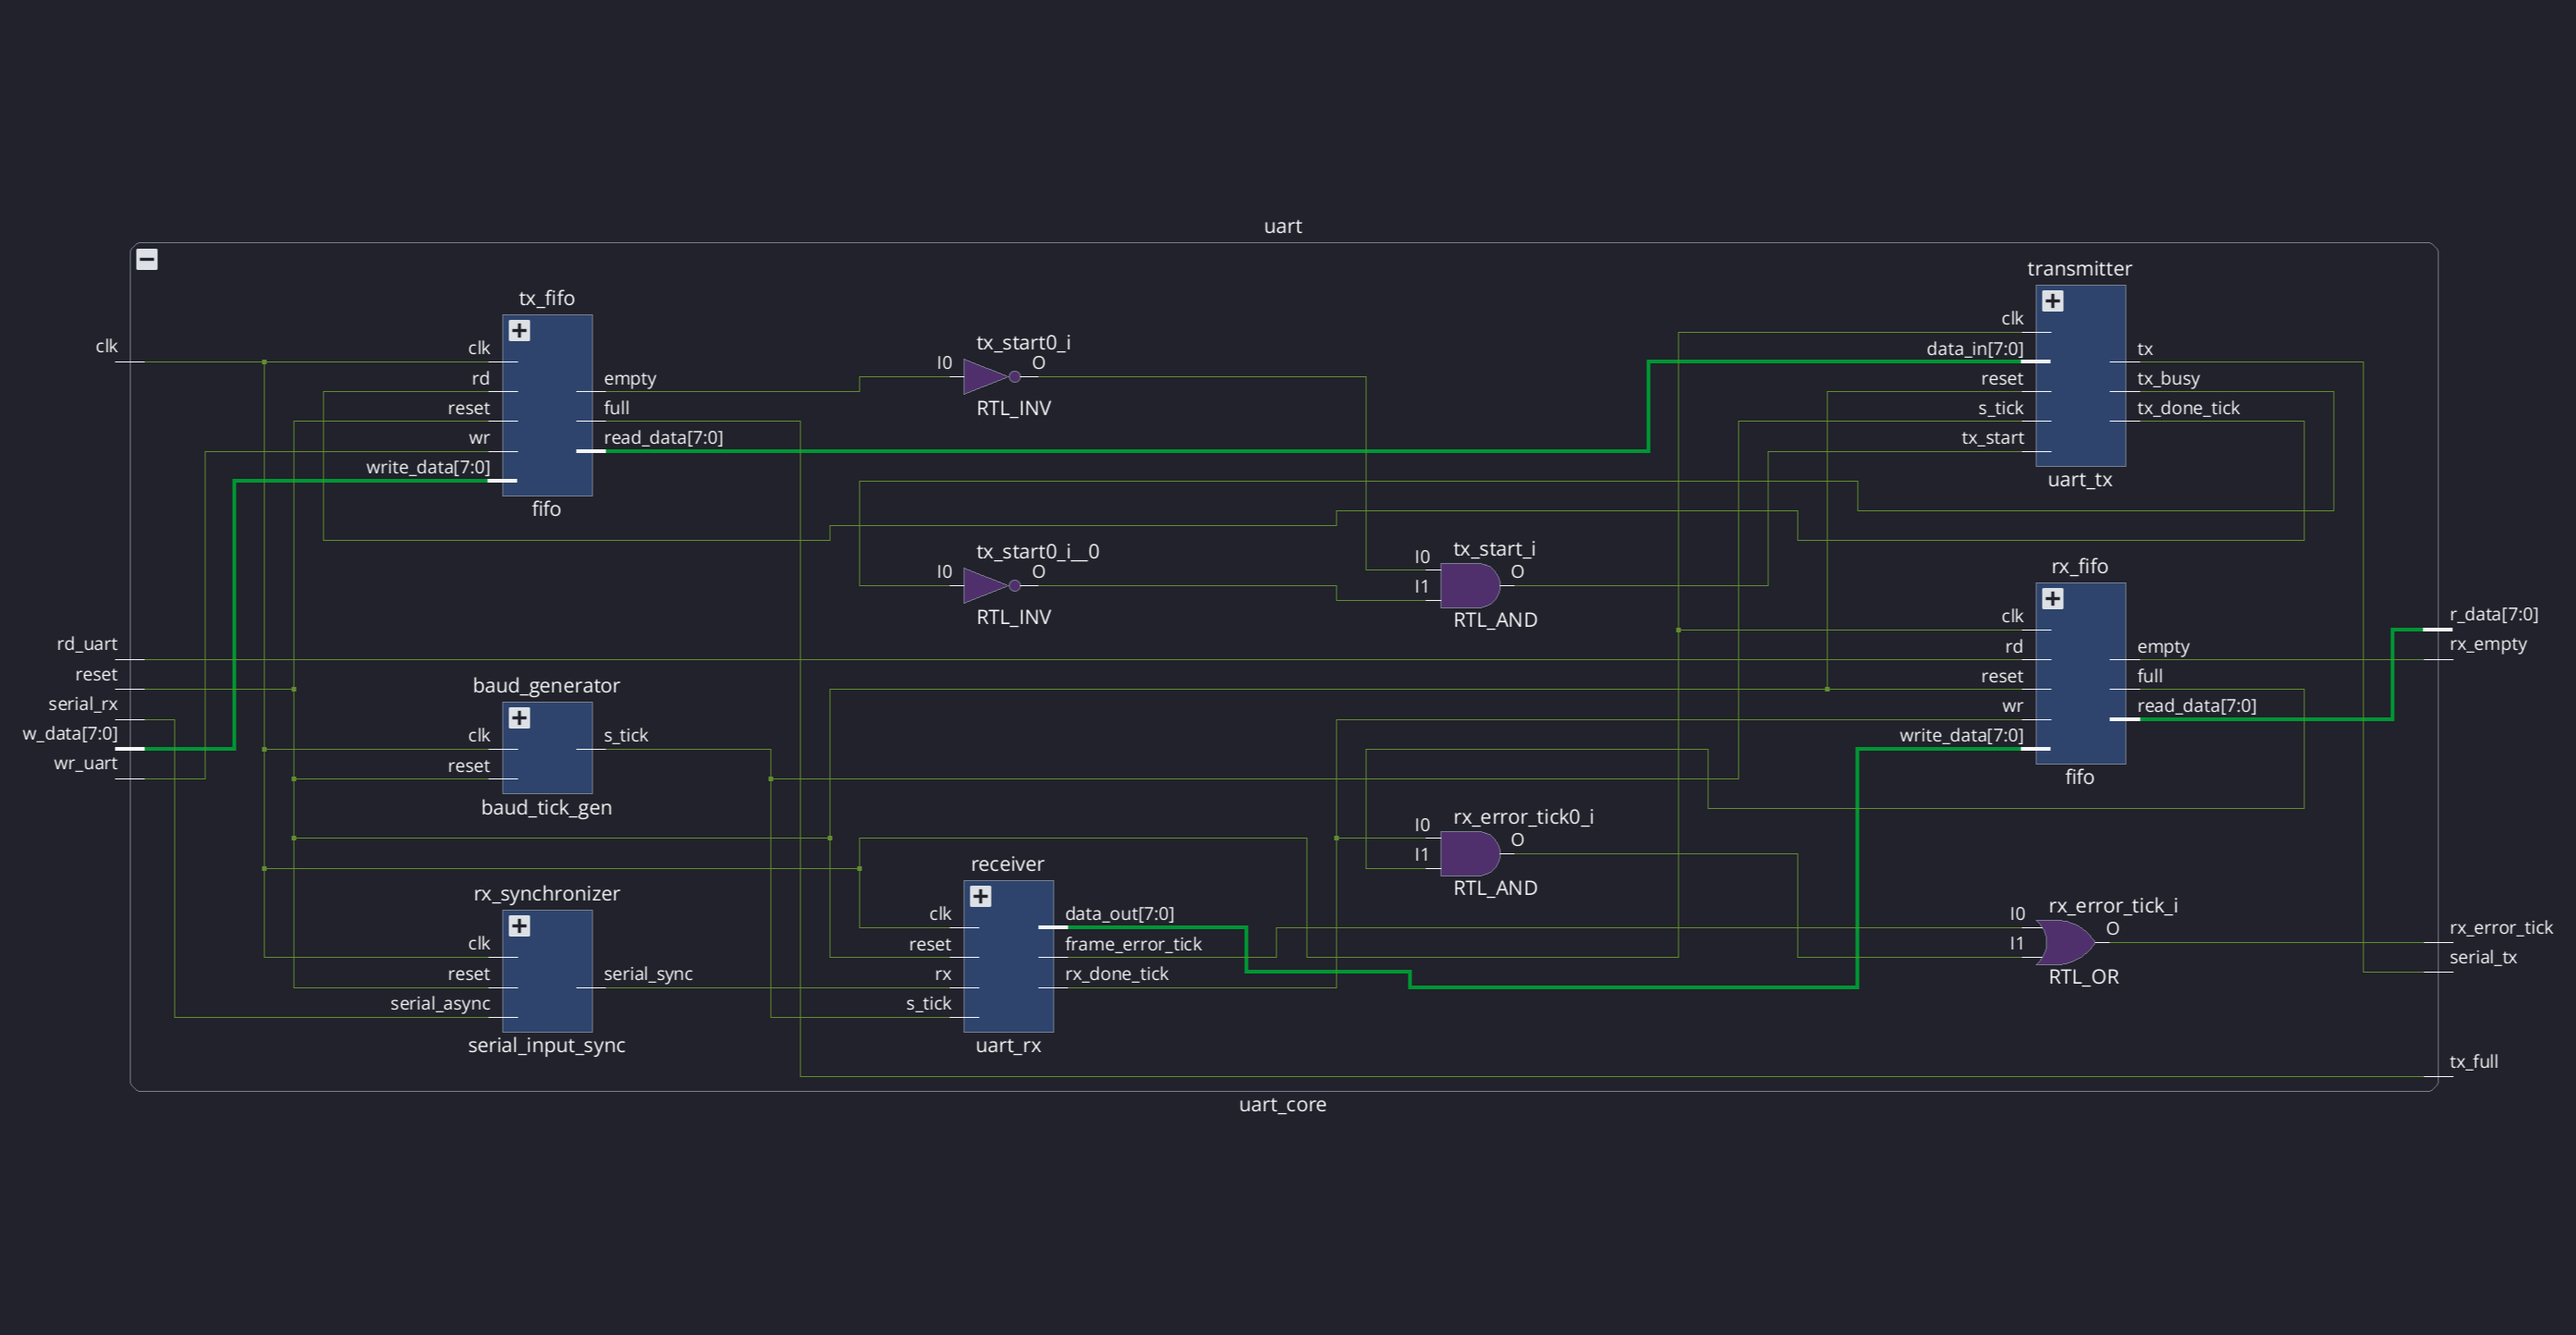
\includegraphics[width=0.92\textwidth]{img/vivado_schematic_uart_core_rtl.png}
  \caption{Esquemático RTL elaborado de \texttt{uart\_core}.}%
  \label{fig:schematic-uart-core-rtl}
\end{figure}

Los circuitos que preparan las señales de entrada se revisaron por
separado. La figura~\ref{fig:schematics-conditioning-rtl} reúne el
acondicionador del reset, el sincronizador de \texttt{serial\_rx} y
el generador de \texttt{s\_tick}. Los esquemáticos confirman que
estas funciones permanecen en módulos independientes antes de
conectarse con el resto del sistema.

\begin{figure}[H]
  \centering
  \begin{minipage}[t]{0.49\textwidth}
    \centering
    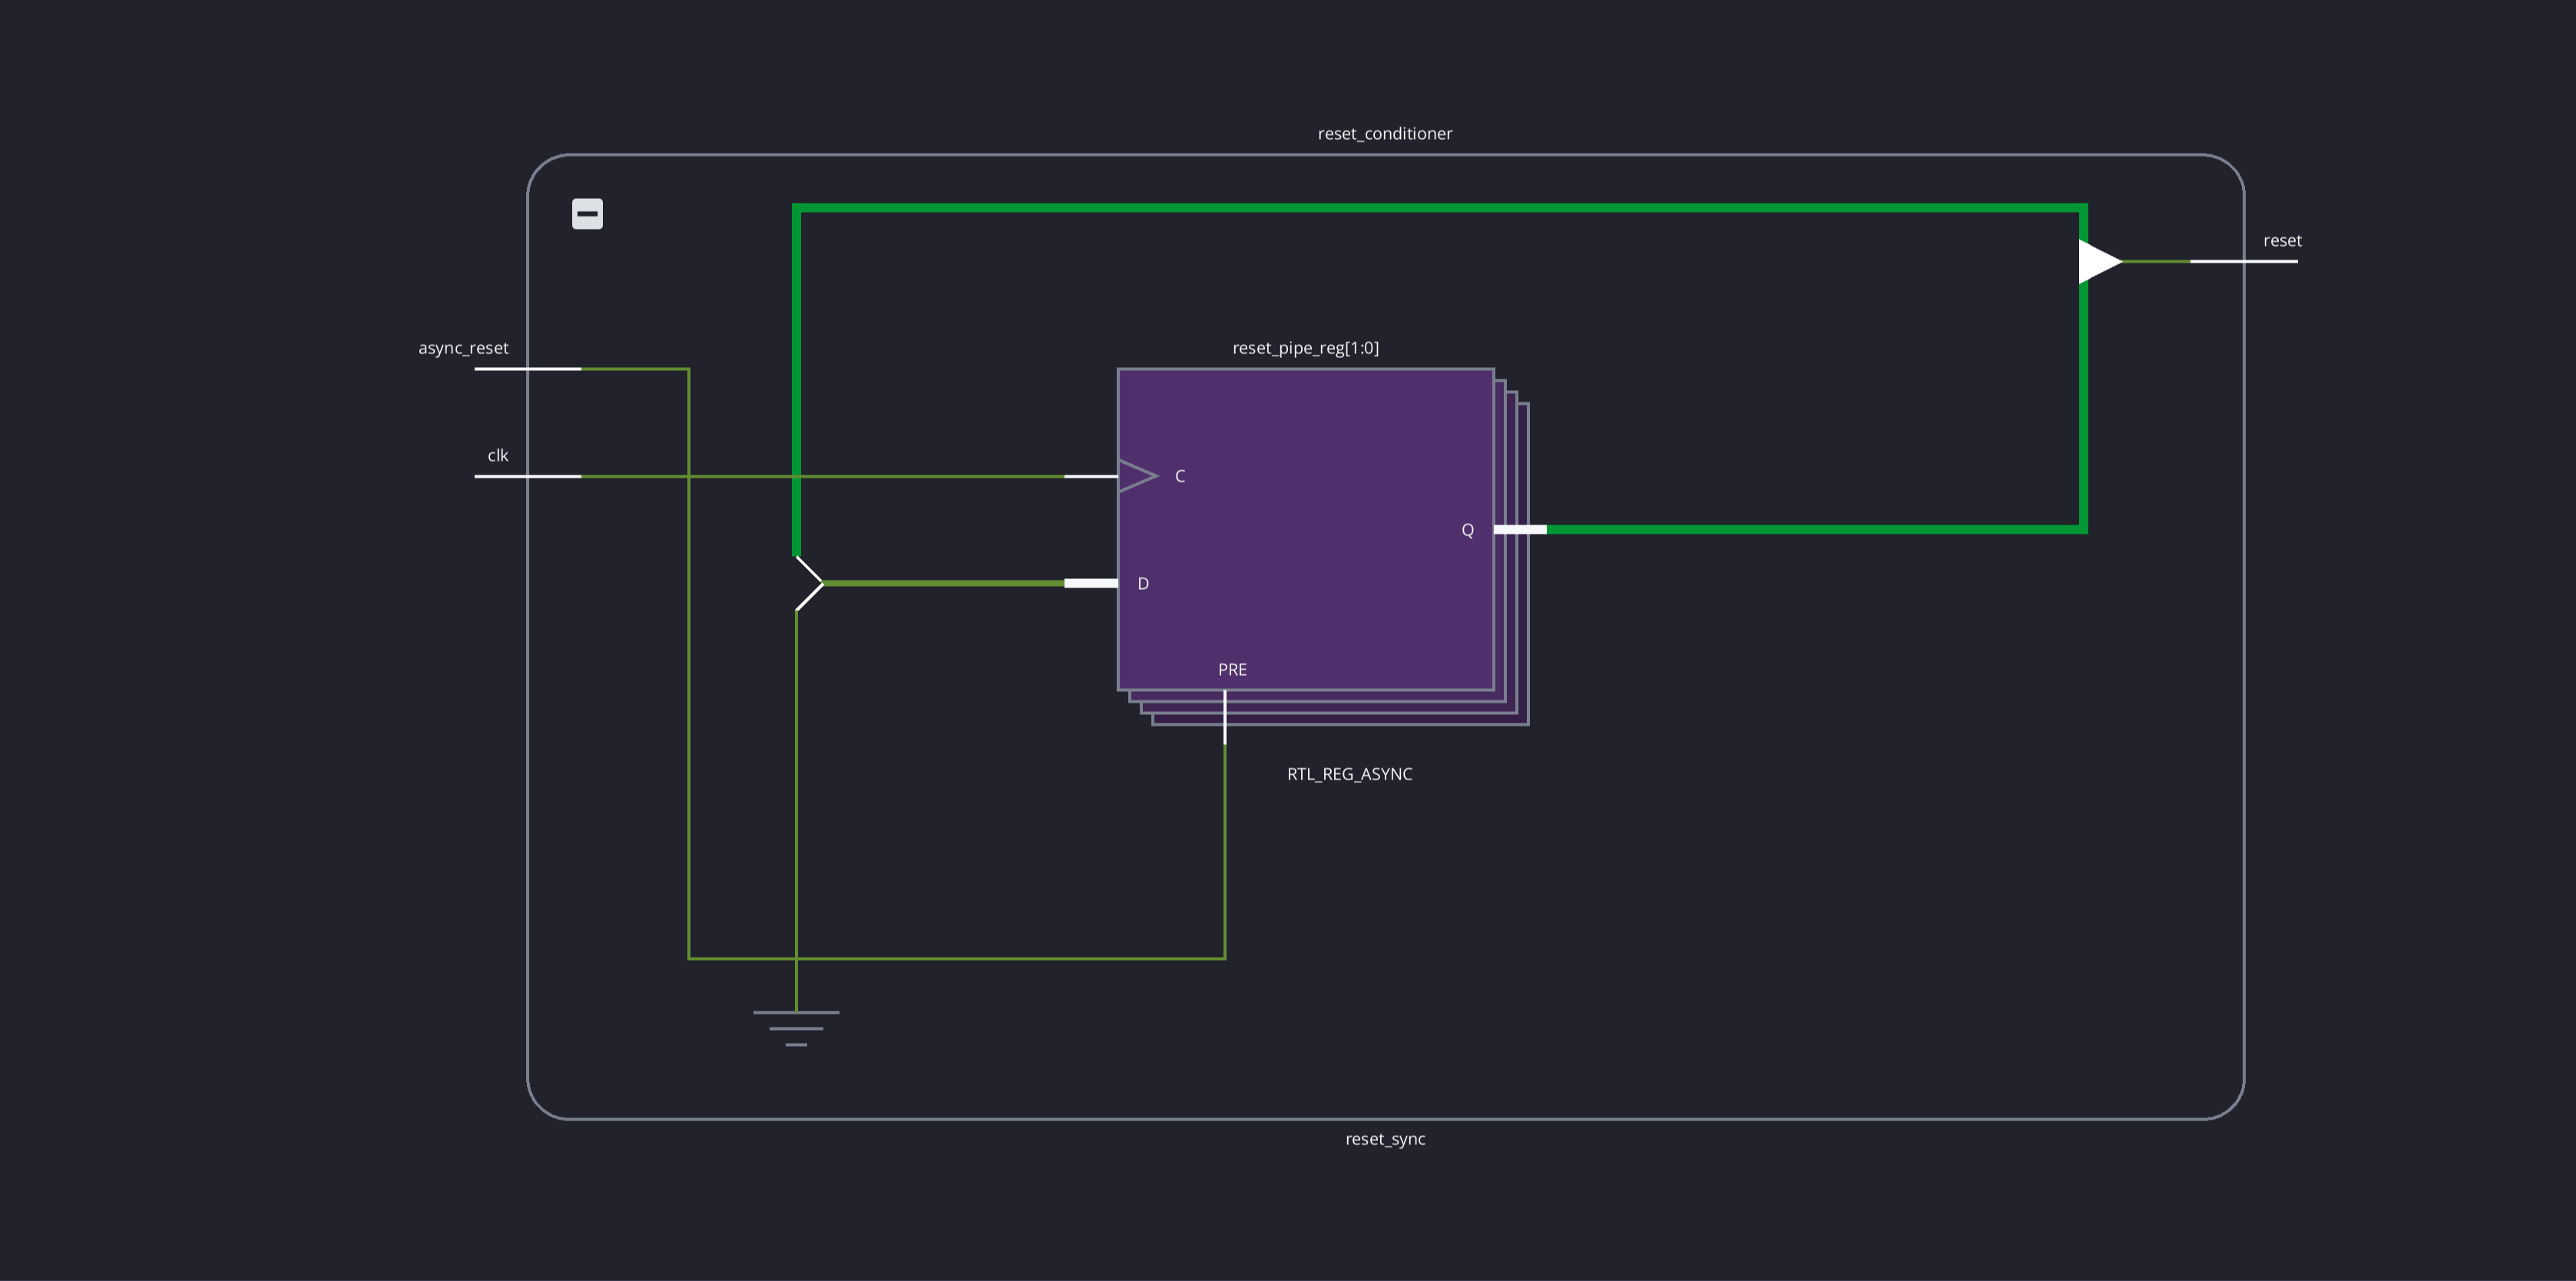
\includegraphics[width=\linewidth]{img/vivado_schematic_reset_sync_rtl.png}
  \end{minipage}\hfill
  \begin{minipage}[t]{0.49\textwidth}
    \centering
    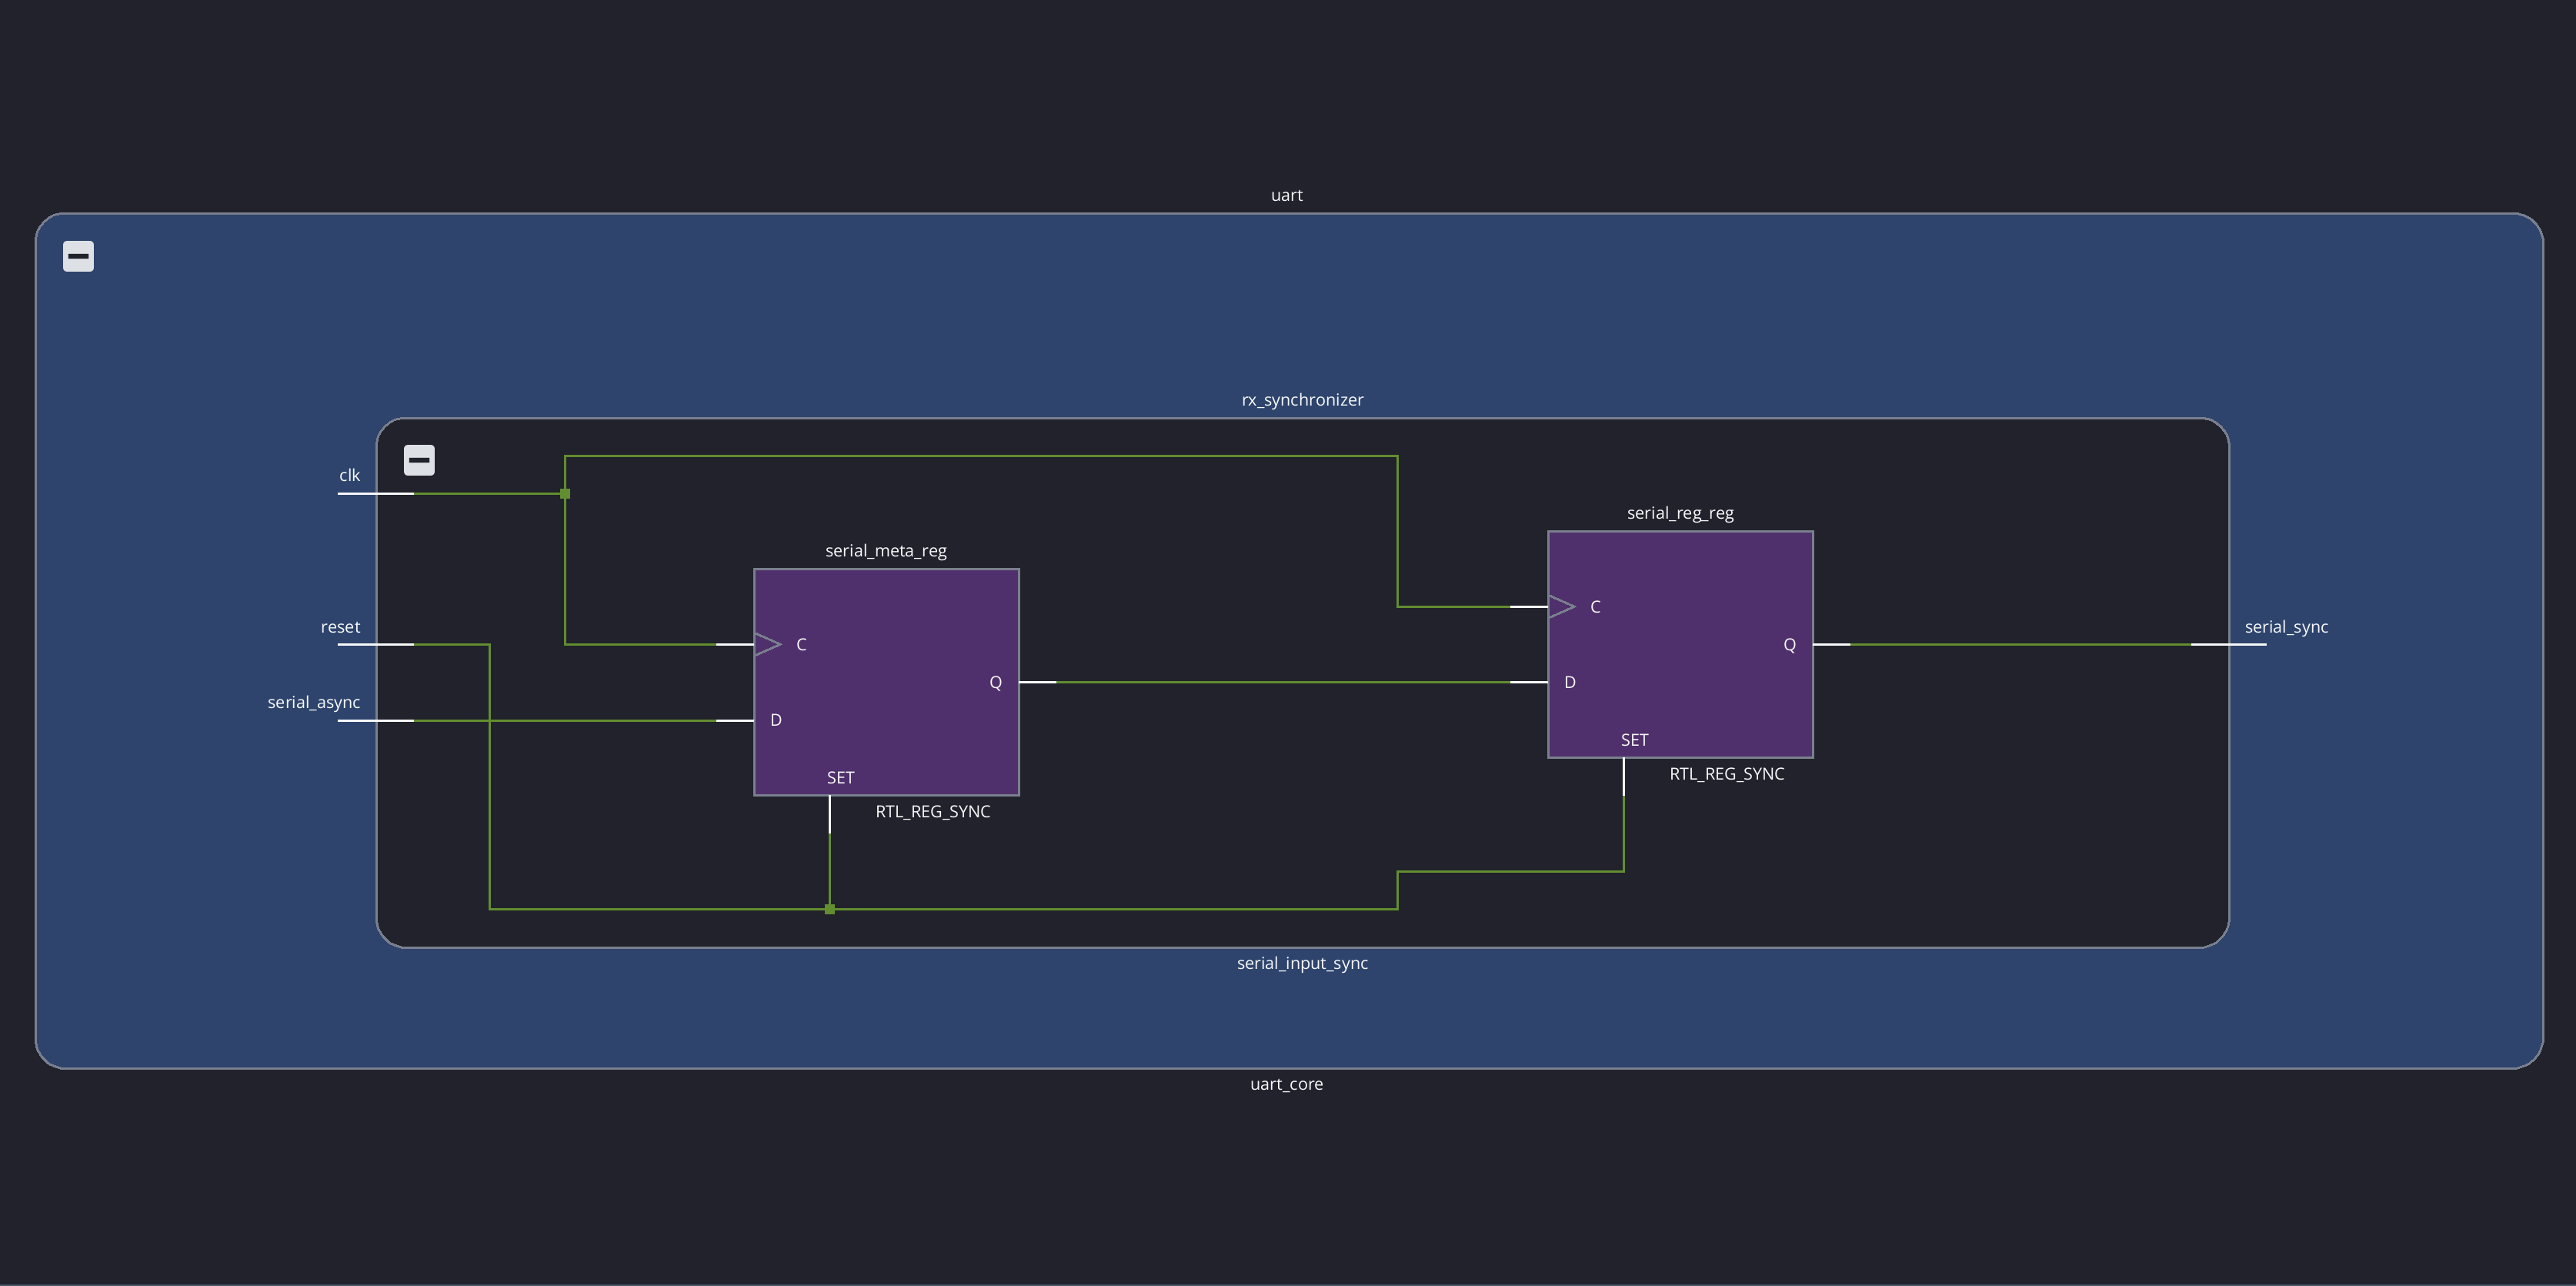
\includegraphics[width=\linewidth]{img/vivado_schematic_serial_input_sync_rtl.png}
  \end{minipage}
  \vspace{0.6em}

  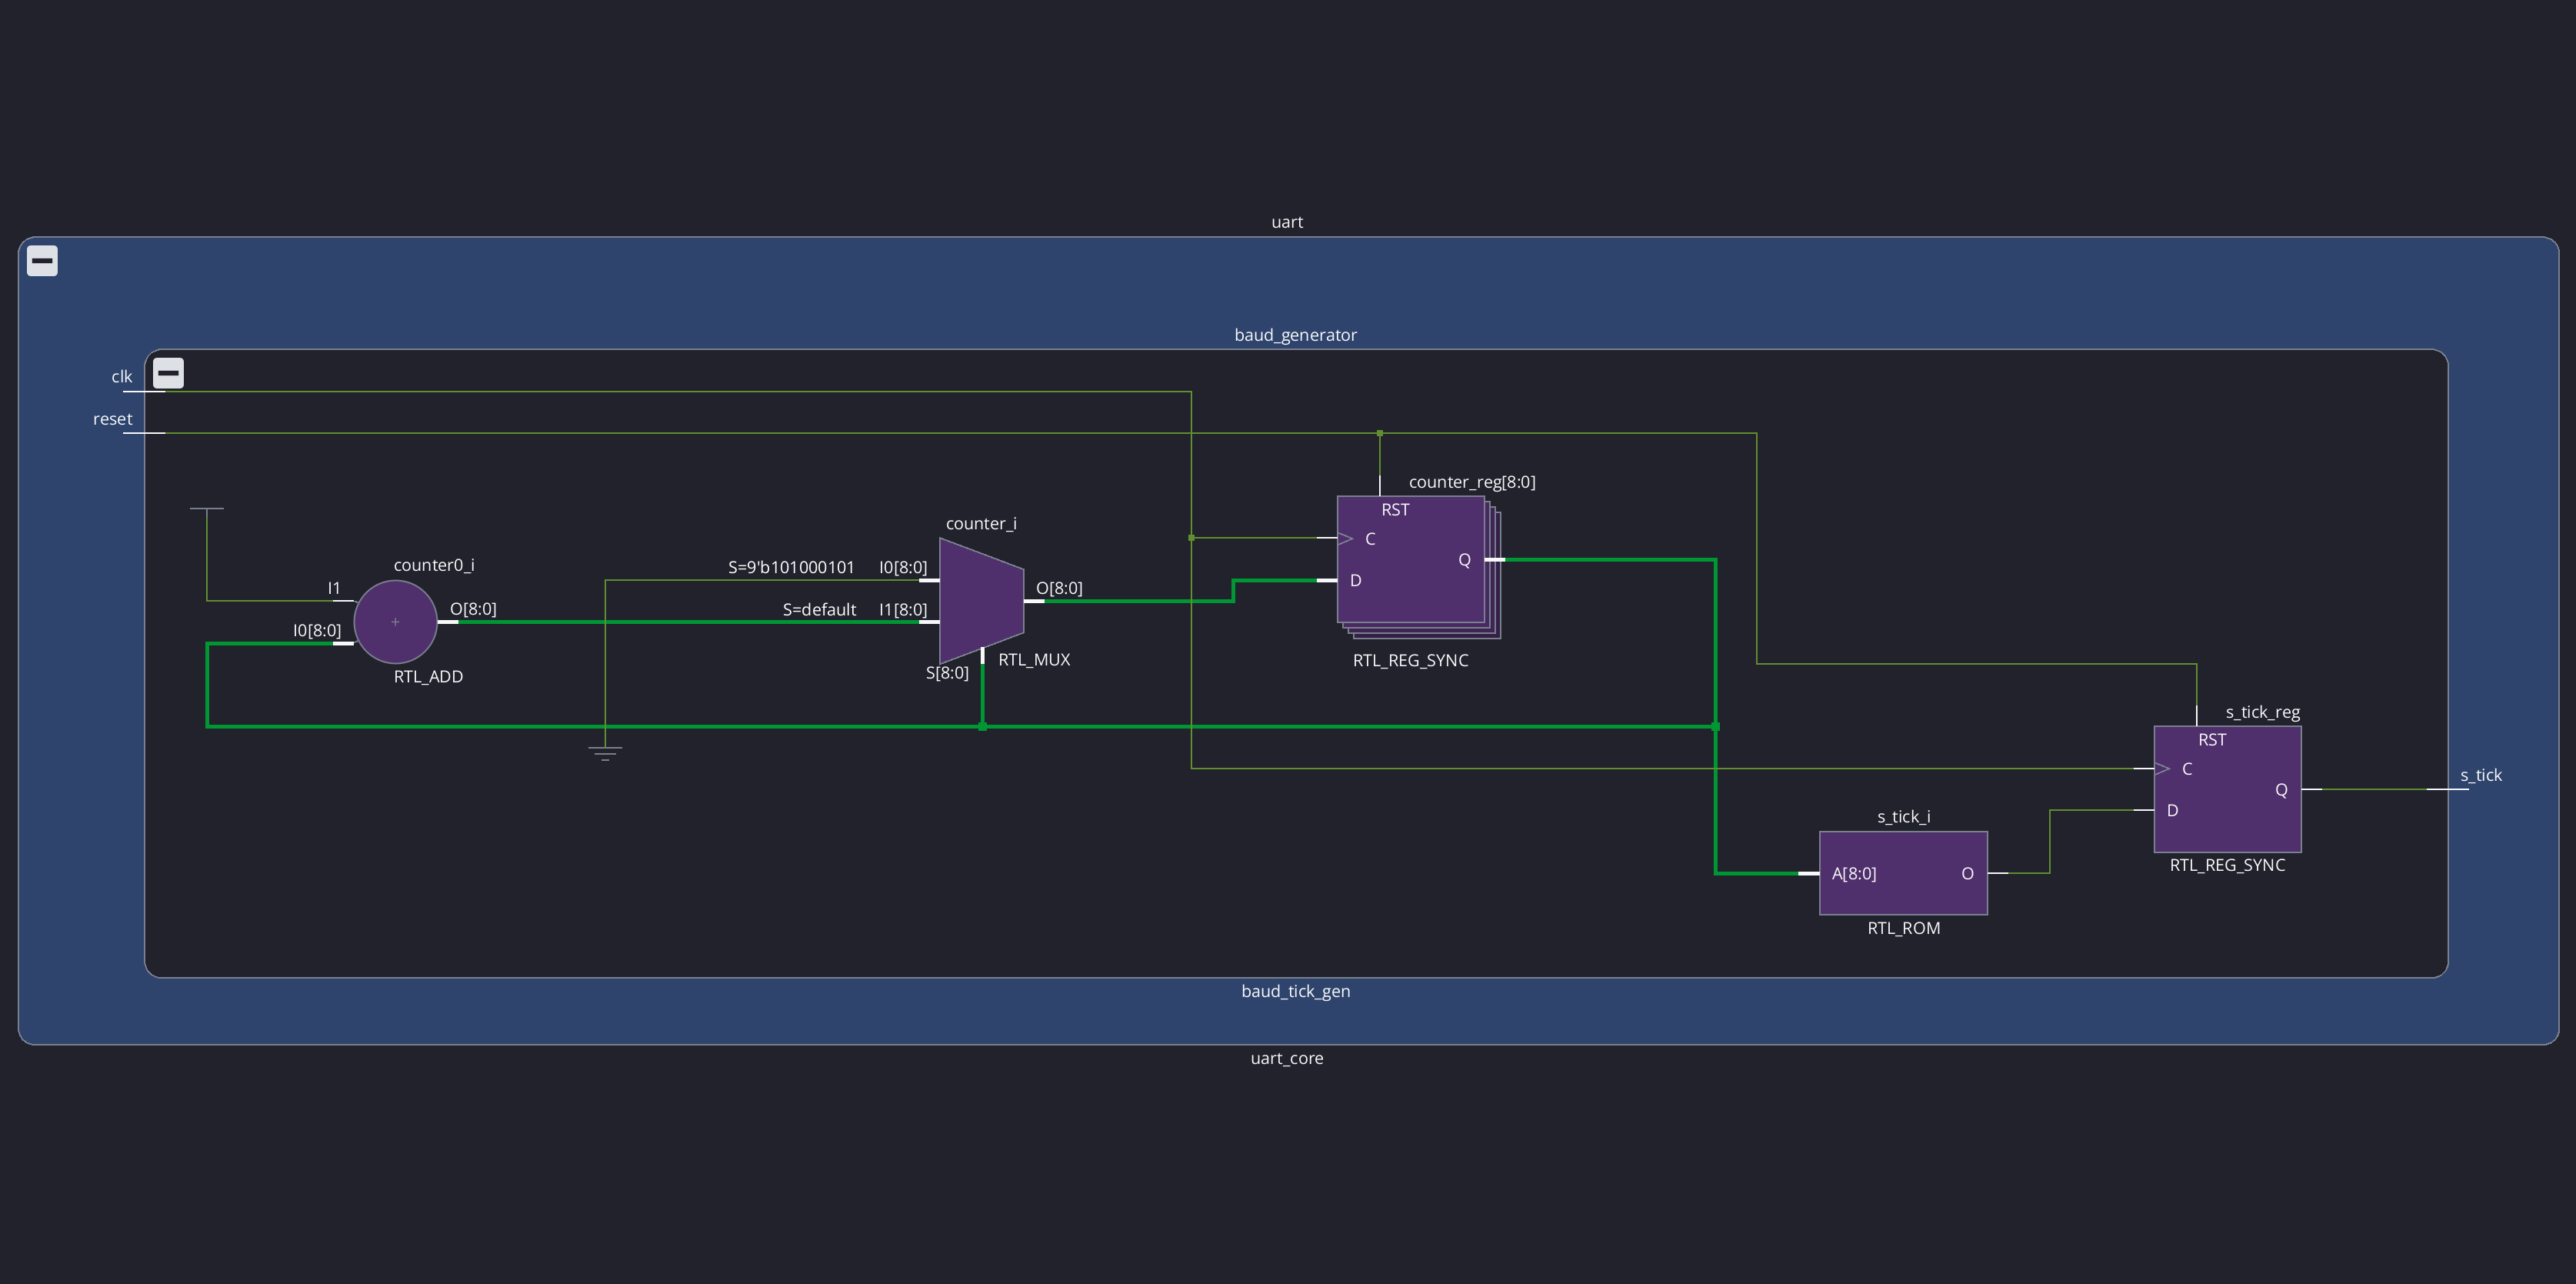
\includegraphics[width=0.72\textwidth]{img/vivado_schematic_baud_tick_gen_rtl.png}
  \caption{Esquemáticos RTL del acondicionamiento de reset, el sincronizador de
  entrada y el generador de muestreo.}%
  \label{fig:schematics-conditioning-rtl}
\end{figure}

La figura~\ref{fig:schematics-rx-tx-rtl} presenta los dos módulos que
forman y reconstruyen las tramas. El esquemático de \texttt{uart\_rx}
corresponde al camino que convierte la entrada serie en un byte. El
de \texttt{uart\_tx} muestra el recorrido inverso desde un byte hasta
la salida serie.

\begin{figure}[H]
  \centering
  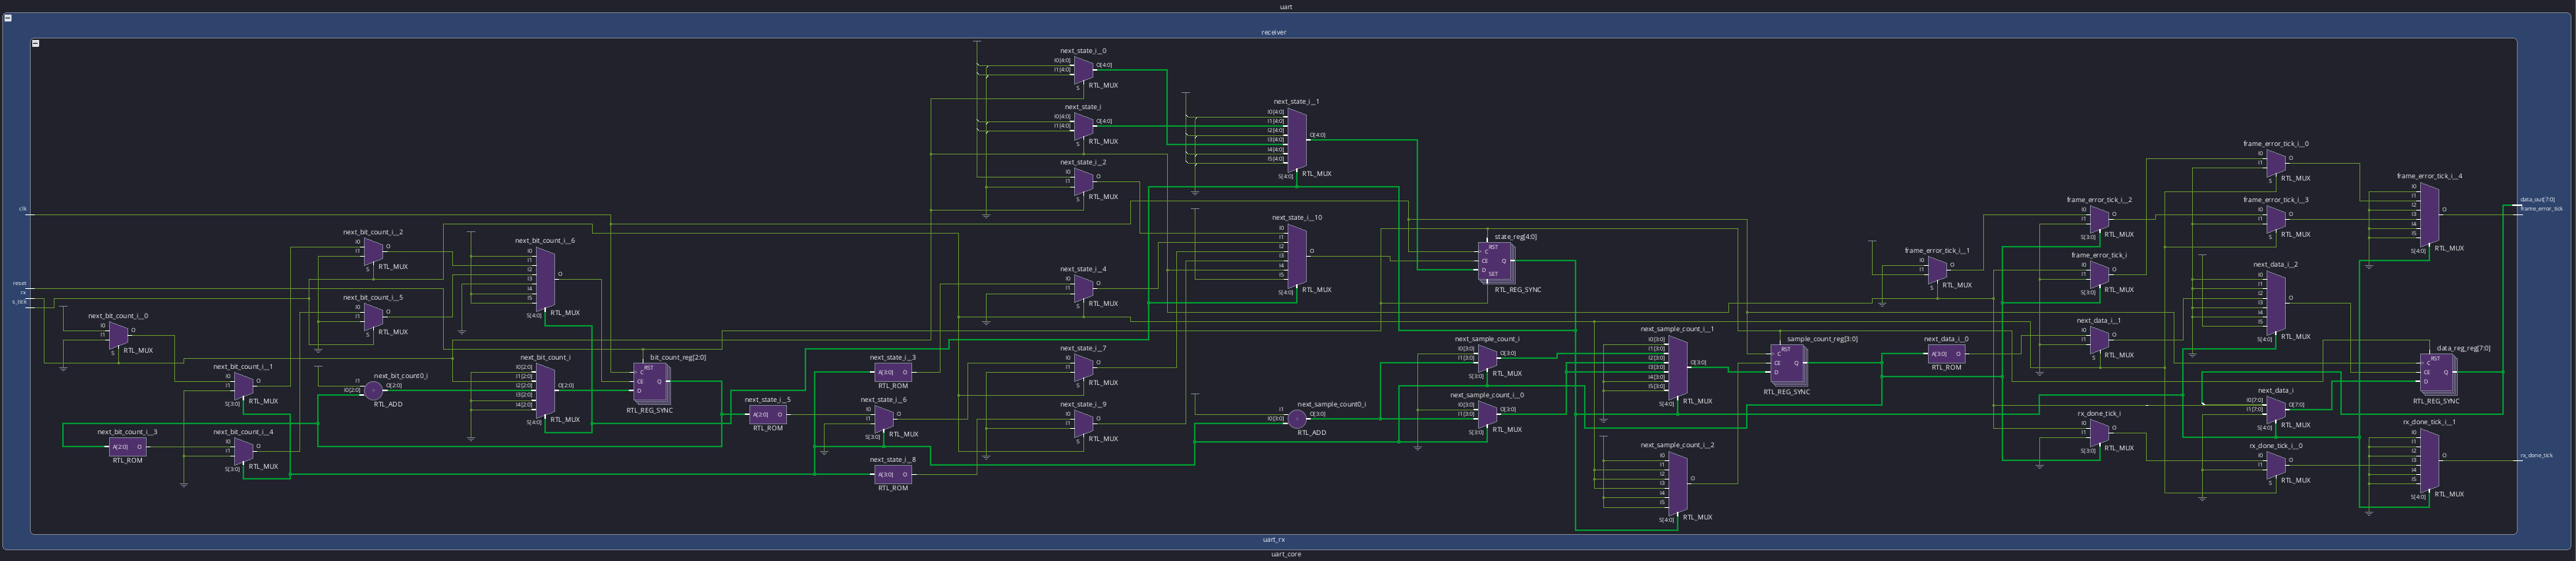
\includegraphics[width=\textwidth]{img/vivado_schematic_uart_rx_rtl.png}
  \vspace{0.6em}

  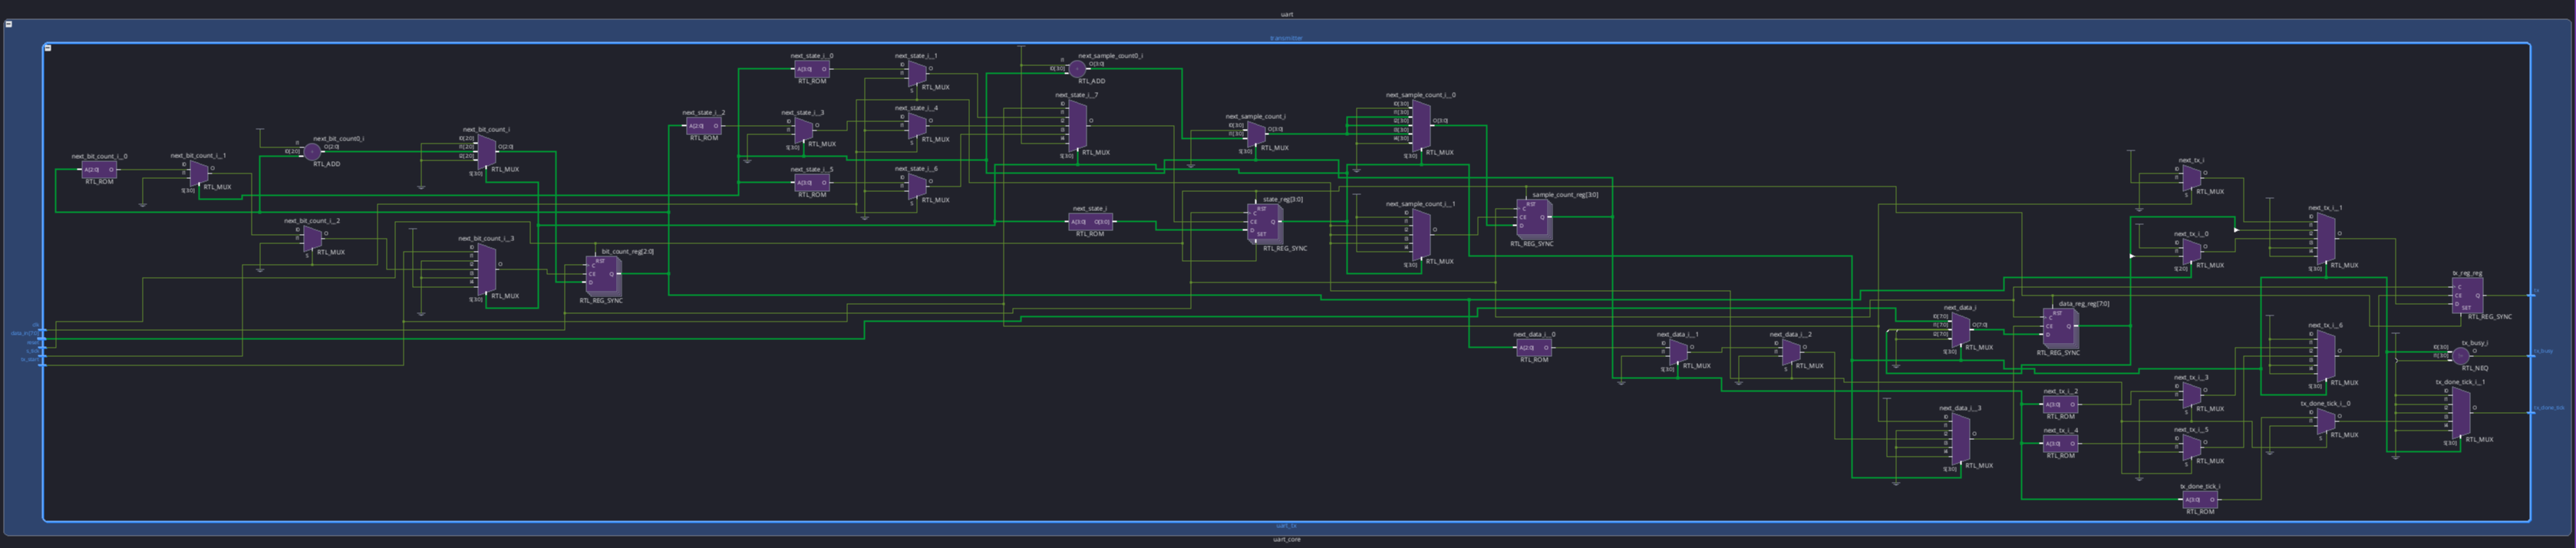
\includegraphics[width=\textwidth]{img/vivado_schematic_uart_tx_rtl.png}
  \caption{Esquemáticos RTL del receptor y del transmisor UART.}%
  \label{fig:schematics-rx-tx-rtl}
\end{figure}

Entre los módulos UART y el controlador se encuentran las dos
instancias de \texttt{fifo}. La figura~\ref{fig:schematics-fifo-rtl}
permite comparar la cola de recepción con la de transmisión. Ambas
conservan la misma estructura, aunque cada una almacena los bytes de
un sentido diferente del enlace.

\begin{figure}[H]
  \centering
  \begin{minipage}[t]{0.49\textwidth}
    \centering
    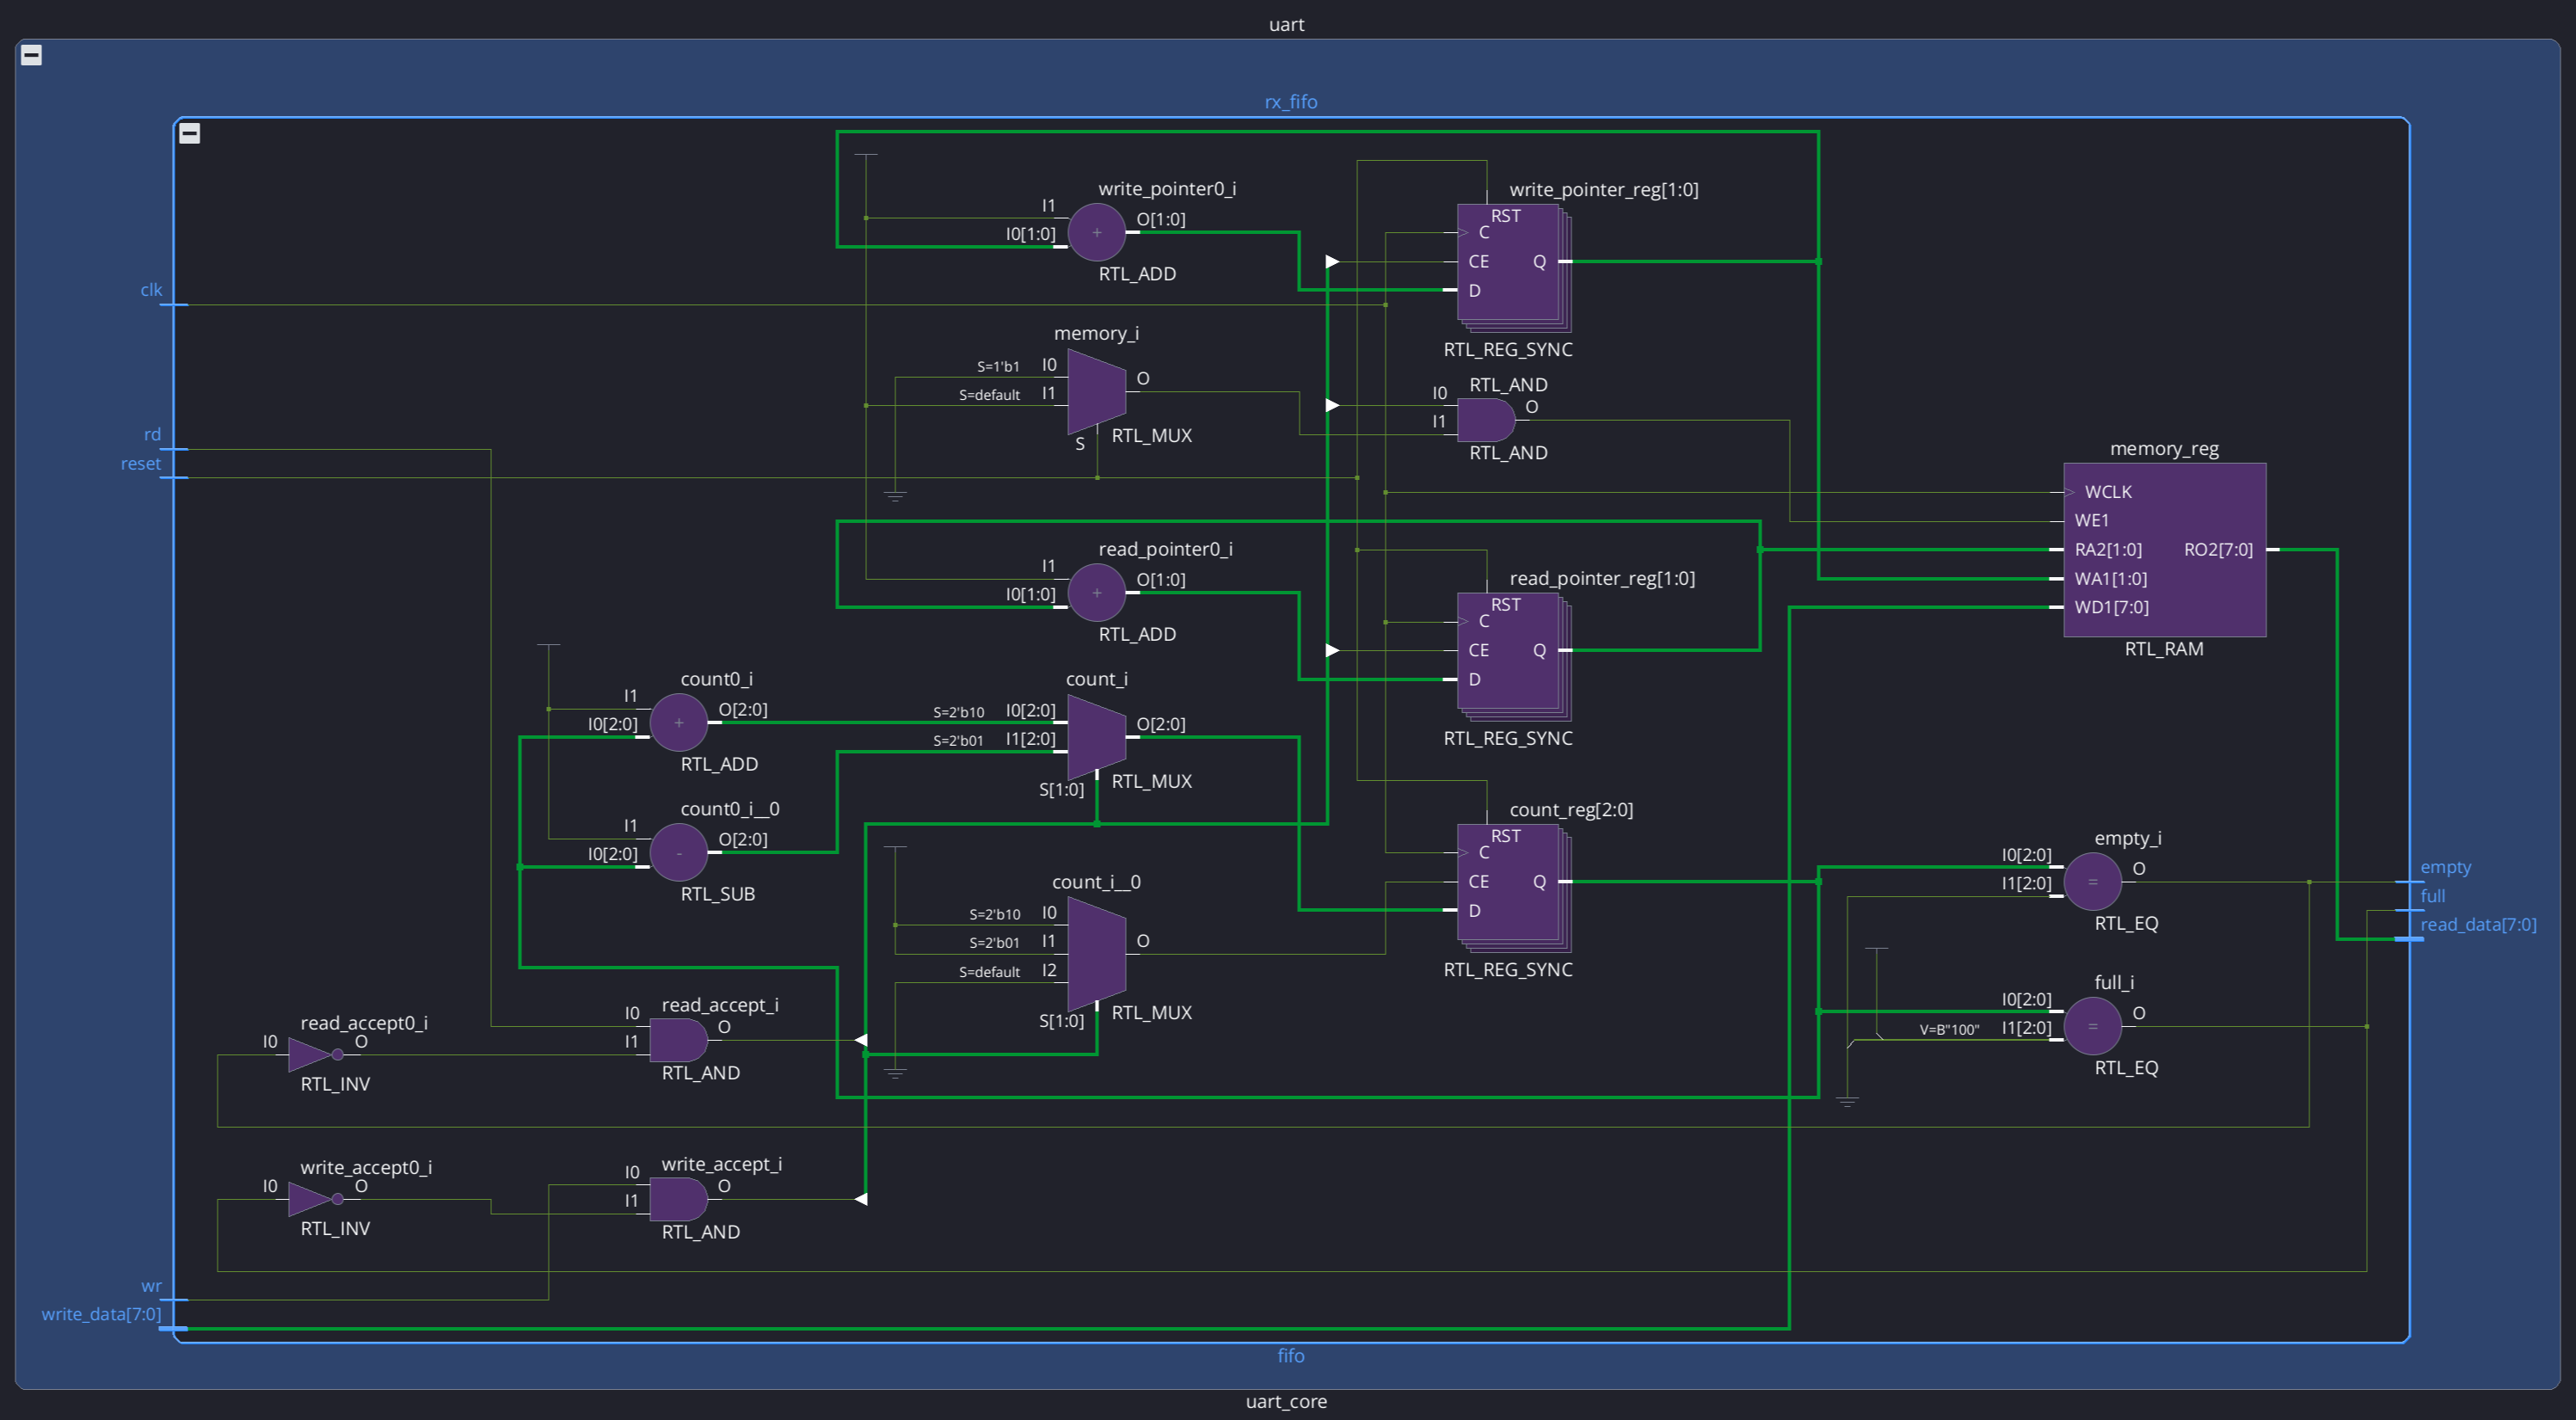
\includegraphics[width=\linewidth]{img/vivado_schematic_rx_fifo_rtl.png}
  \end{minipage}\hfill
  \begin{minipage}[t]{0.49\textwidth}
    \centering
    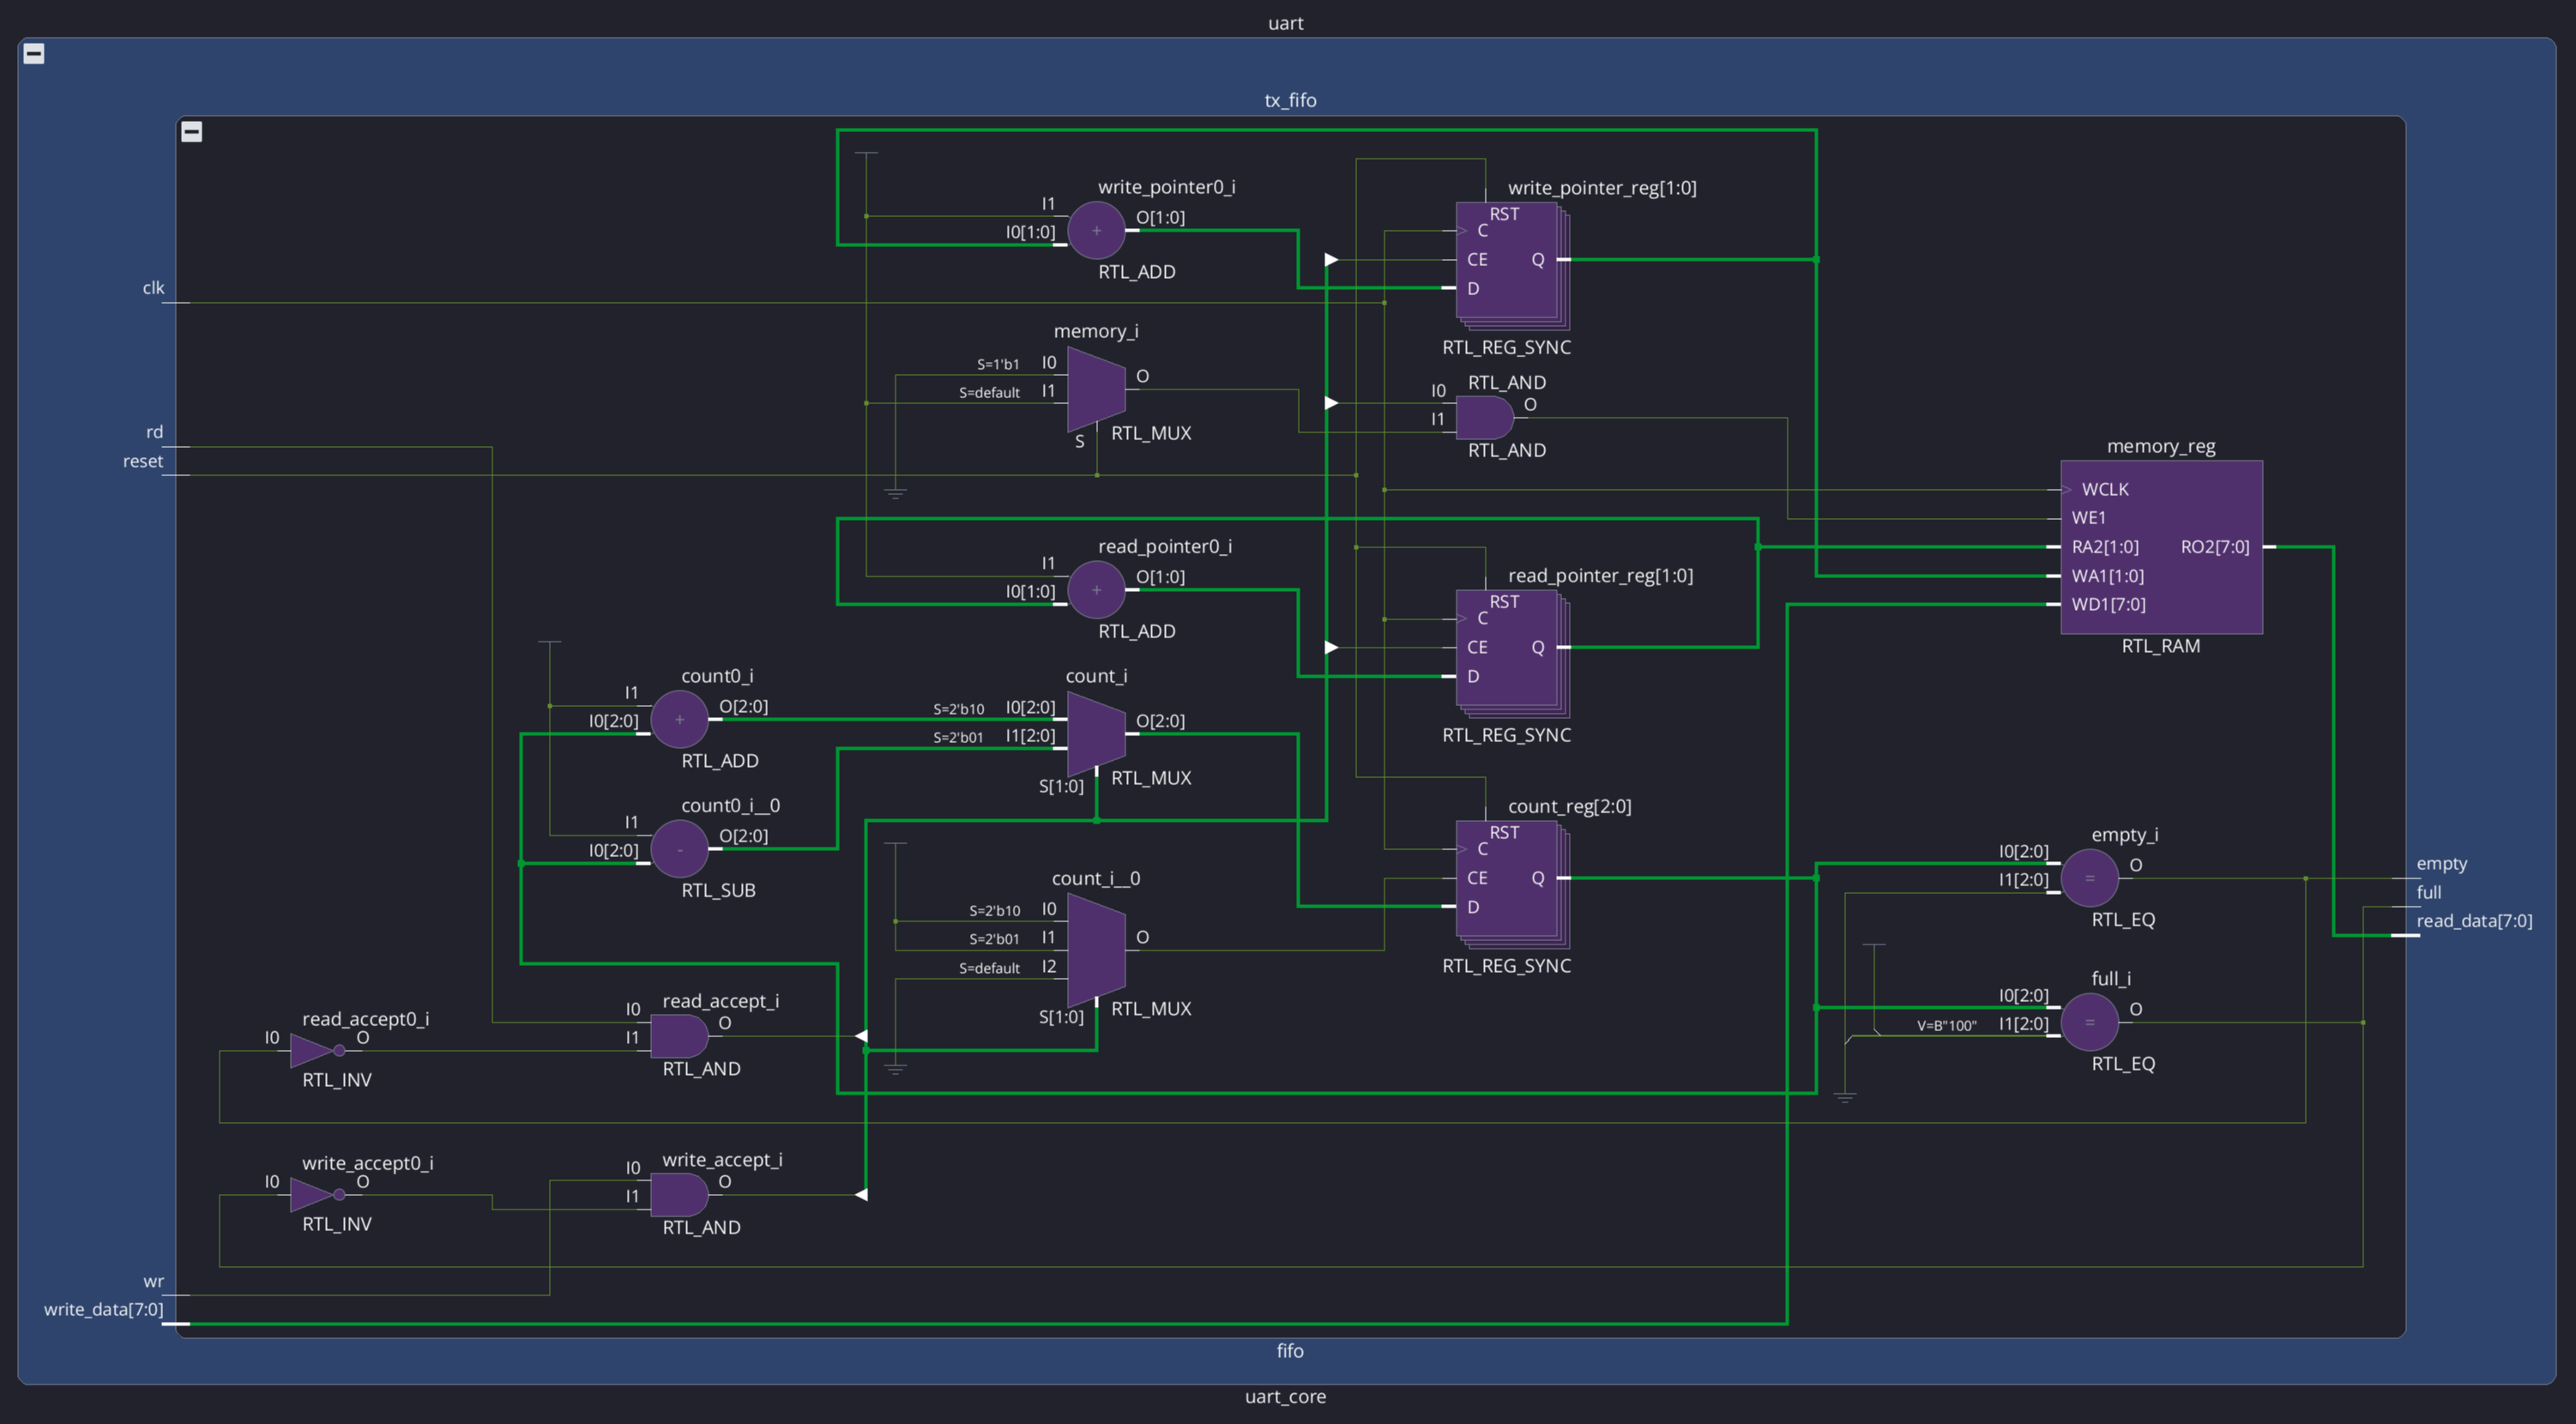
\includegraphics[width=\linewidth]{img/vivado_schematic_tx_fifo_rtl.png}
  \end{minipage}
  \caption{Esquemáticos RTL de las instancias FIFO de recepción y transmisión.}%
  \label{fig:schematics-fifo-rtl}
\end{figure}

Una vez reconstruidos los bytes, el controlador debe interpretar la
solicitud y coordinar la respuesta. La
figura~\ref{fig:schematic-controller-rtl} muestra la estructura
elaborada a partir del archivo
\texttt{rtl/alu\allowbreak\_uart\allowbreak\_controller.sv}. En ella
se mantienen diferenciados los registros de la transacción y la
lógica que controla su avance.

\begin{figure}[H]
  \centering
  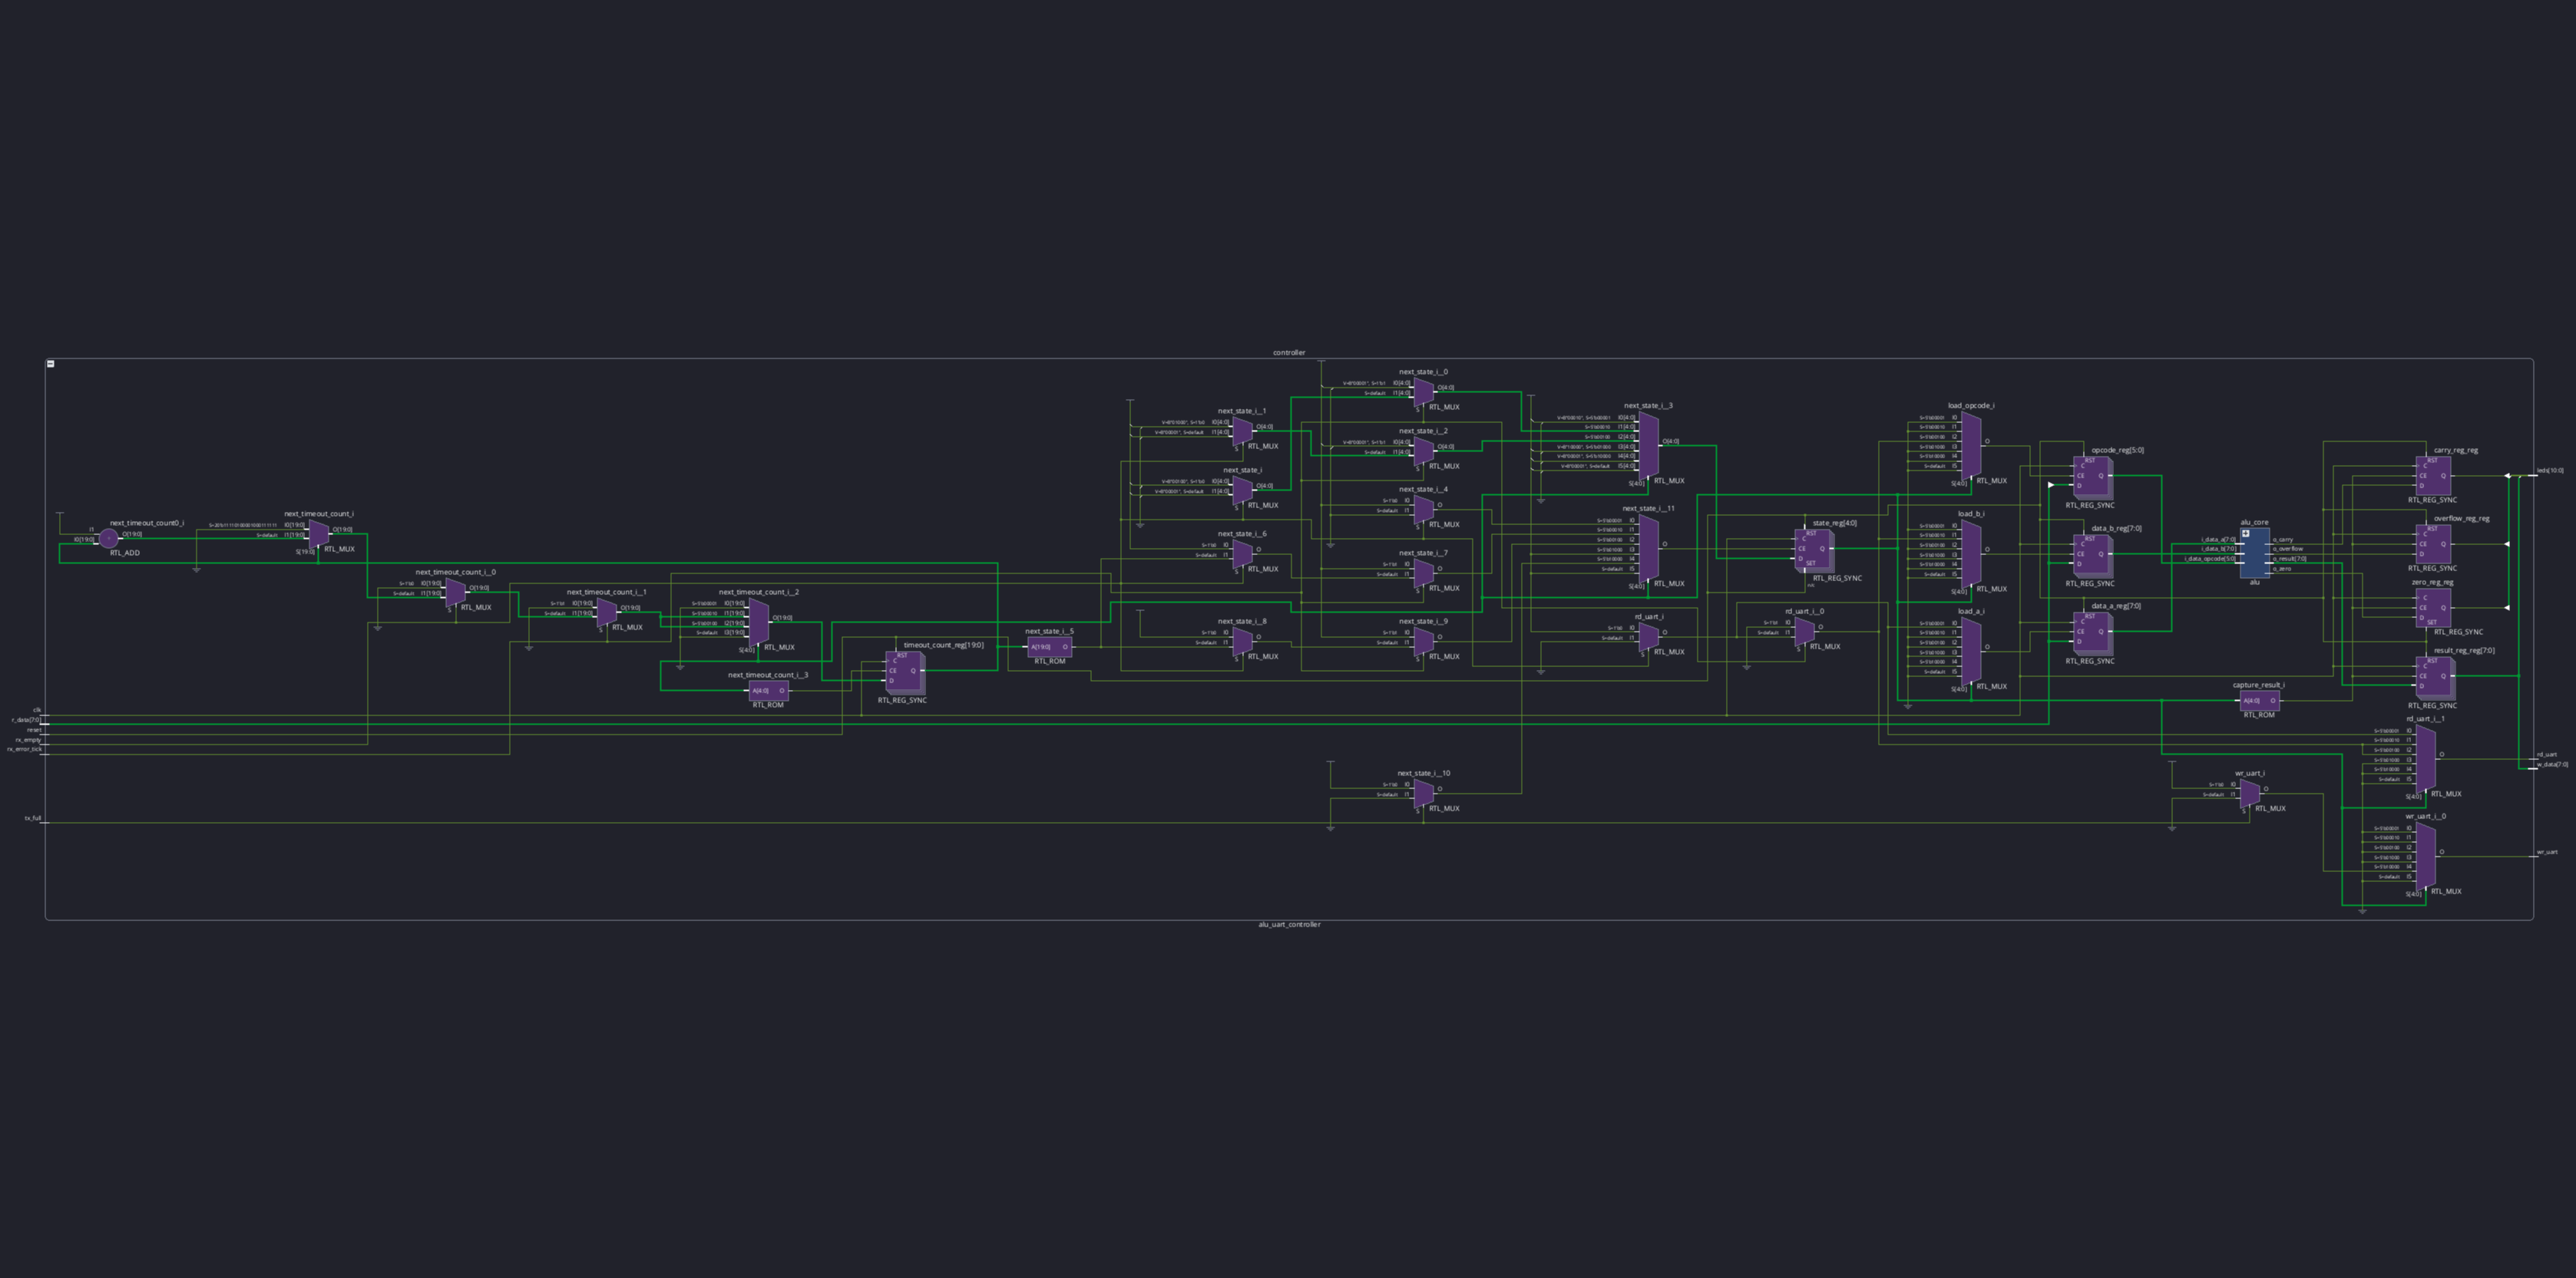
\includegraphics[width=\textwidth]{img/vivado_schematic_controller_rtl.png}
  \caption{Esquemático RTL elaborado del controlador de transacciones.}%
  \label{fig:schematic-controller-rtl}
\end{figure}

La última parte del camino corresponde al cálculo. El esquemático de
la figura~\ref{fig:schematic-alu-rtl} muestra la ALU combinacional
elaborada desde \texttt{rtl/alu.sv}. La ausencia de registros dentro
de este bloque coincide con la decisión de almacenar el resultado y
las banderas en el controlador.

\begin{figure}[H]
  \centering
  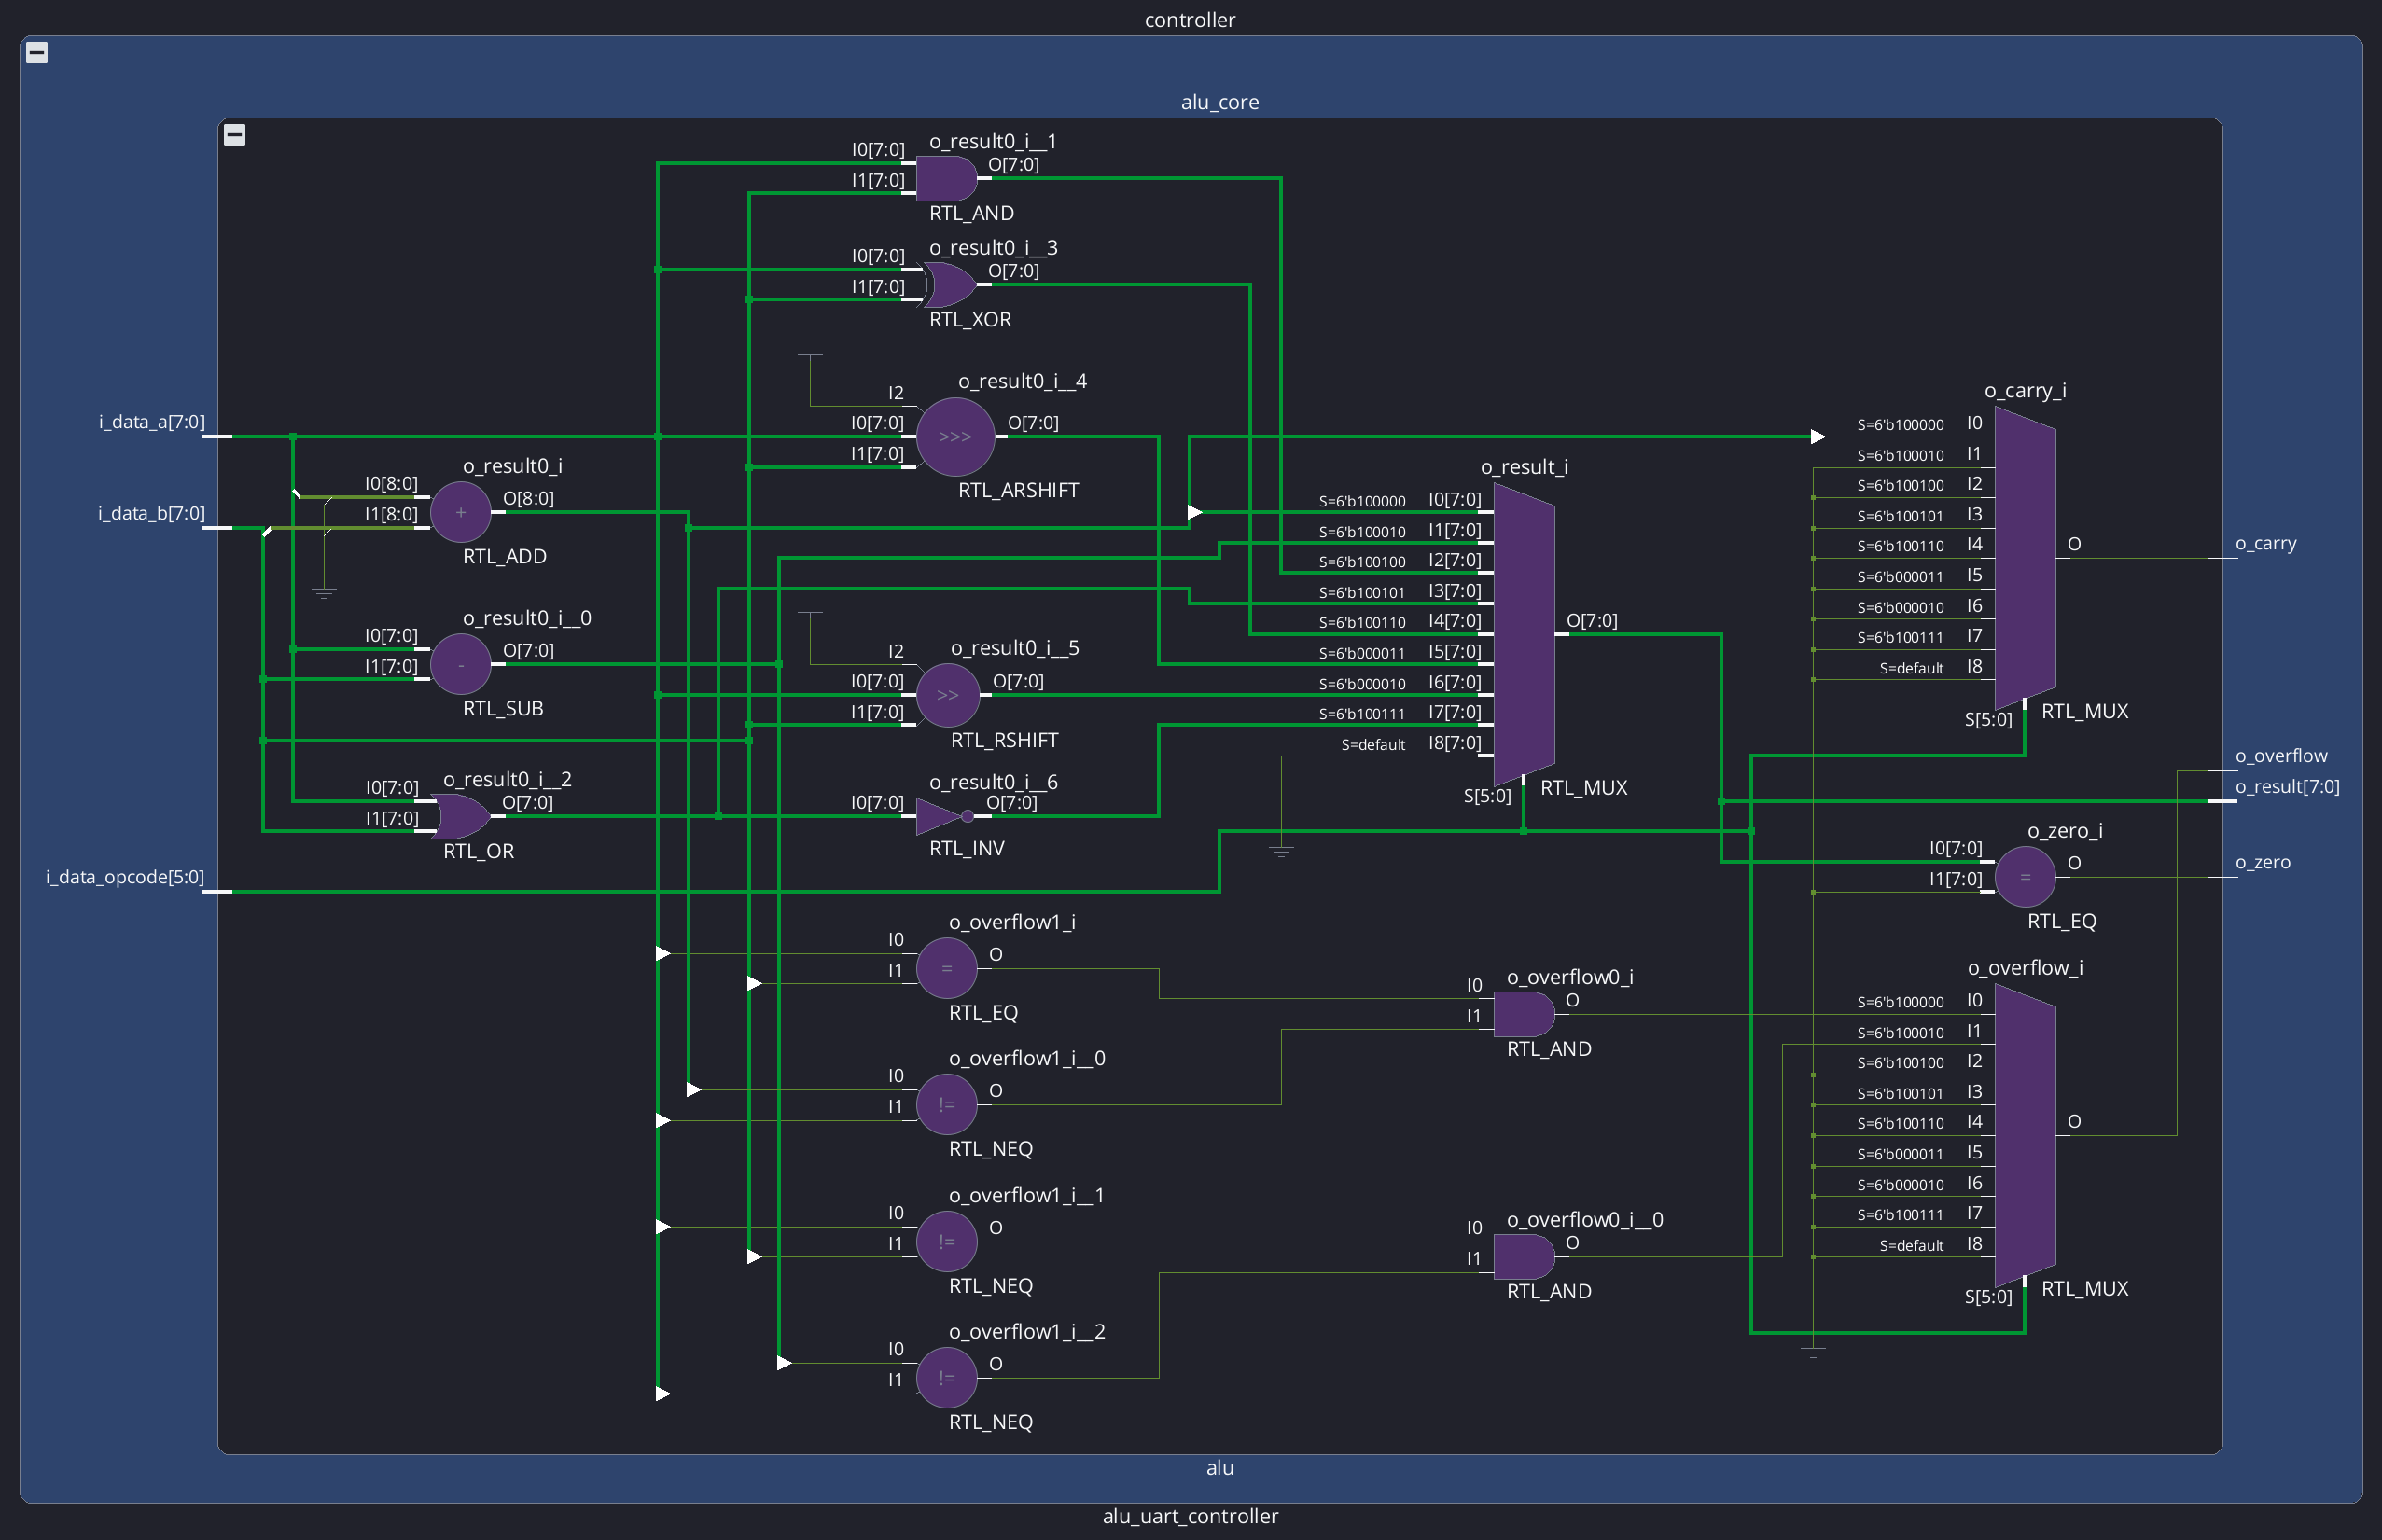
\includegraphics[width=0.78\textwidth]{img/vivado_schematic_alu_rtl.png}
  \caption{Esquemático RTL elaborado de la ALU combinacional.}%
  \label{fig:schematic-alu-rtl}
\end{figure}

En conjunto, estos esquemáticos muestran que la elaboración conservó
la separación prevista entre la comunicación UART, el almacenamiento,
el control de la transacción y el cálculo.

\section{Del esquema RTL a los recursos físicos}

Después de comprobar la jerarquía elaborada, se analizó la forma en
que Vivado la convirtió en recursos del Artix-7. Esta comparación
permite determinar si los registros, las memorias y la lógica
combinacional fueron inferidos de acuerdo con la arquitectura.

Los contadores de sobremuestreo, los índices de bits, el contador del
timeout y los contadores de ocupación necesitan conservar un valor
entre ciclos. Por esta razón aparecen como flip-flops acompañados por
las LUT que calculan su próximo valor.

Las tres máquinas de estado utilizan en total catorce bits. Cinco
corresponden al receptor, cuatro al transmisor y cinco al
controlador. Vivado implementa estos bits con registros y utiliza LUT
para determinar las transiciones. Los catorce bits no representan
estados activos al mismo tiempo. Durante el funcionamiento normal
permanece activo un solo bit de cada máquina.

Cada FIFO contiene un arreglo de cuatro palabras de ocho bits. Debido
a su tamaño, no resulta conveniente utilizar un bloque completo de
memoria. Vivado implementa ambos arreglos como memoria distribuida en
LUTRAM. Esto explica las 12 LUT utilizadas como memoria después del
ruteo y la ausencia de bloques RAM.

La ALU se implementa mediante LUT y cadenas de carry para las
operaciones de suma y resta. No requiere bloques DSP. Los registros
de los operandos, del opcode, del resultado y de las banderas también
forman parte de los 134 flip-flops informados. A esos registros se
suman los utilizados para los desplazamientos y los distintos contadores.

La conexión con la placa utiliza tres buffers de entrada. Estos
corresponden al reloj, el reset y la línea RX. También utiliza doce
buffers de salida para TX y los once LED. En total se ocupan 15 IOB.

El reloj que ingresa por el pin W5 utiliza un único BUFG. El
generador de baud no agrega otro buffer global porque
\texttt{s\_tick} funciona como una habilitación síncrona y no como un
segundo reloj. Si la implementación hubiera incorporado una BRAM, un
DSP o un segundo BUFG, habría sido necesario revisar la inferencia
realizada por la herramienta.

Los esquemáticos implementados permiten observar esta traducción. A
diferencia de la vista RTL, ya no muestran solamente los módulos
descriptos en SystemVerilog. En ellos aparecen los registros, las
LUT, las cadenas de carry y las conexiones adaptadas al dispositivo
después de la colocación y el ruteo.

La figura~\ref{fig:schematic-top-implemented} presenta la vista
general del nivel superior ya implementado.

\begin{figure}[H]
  \centering
  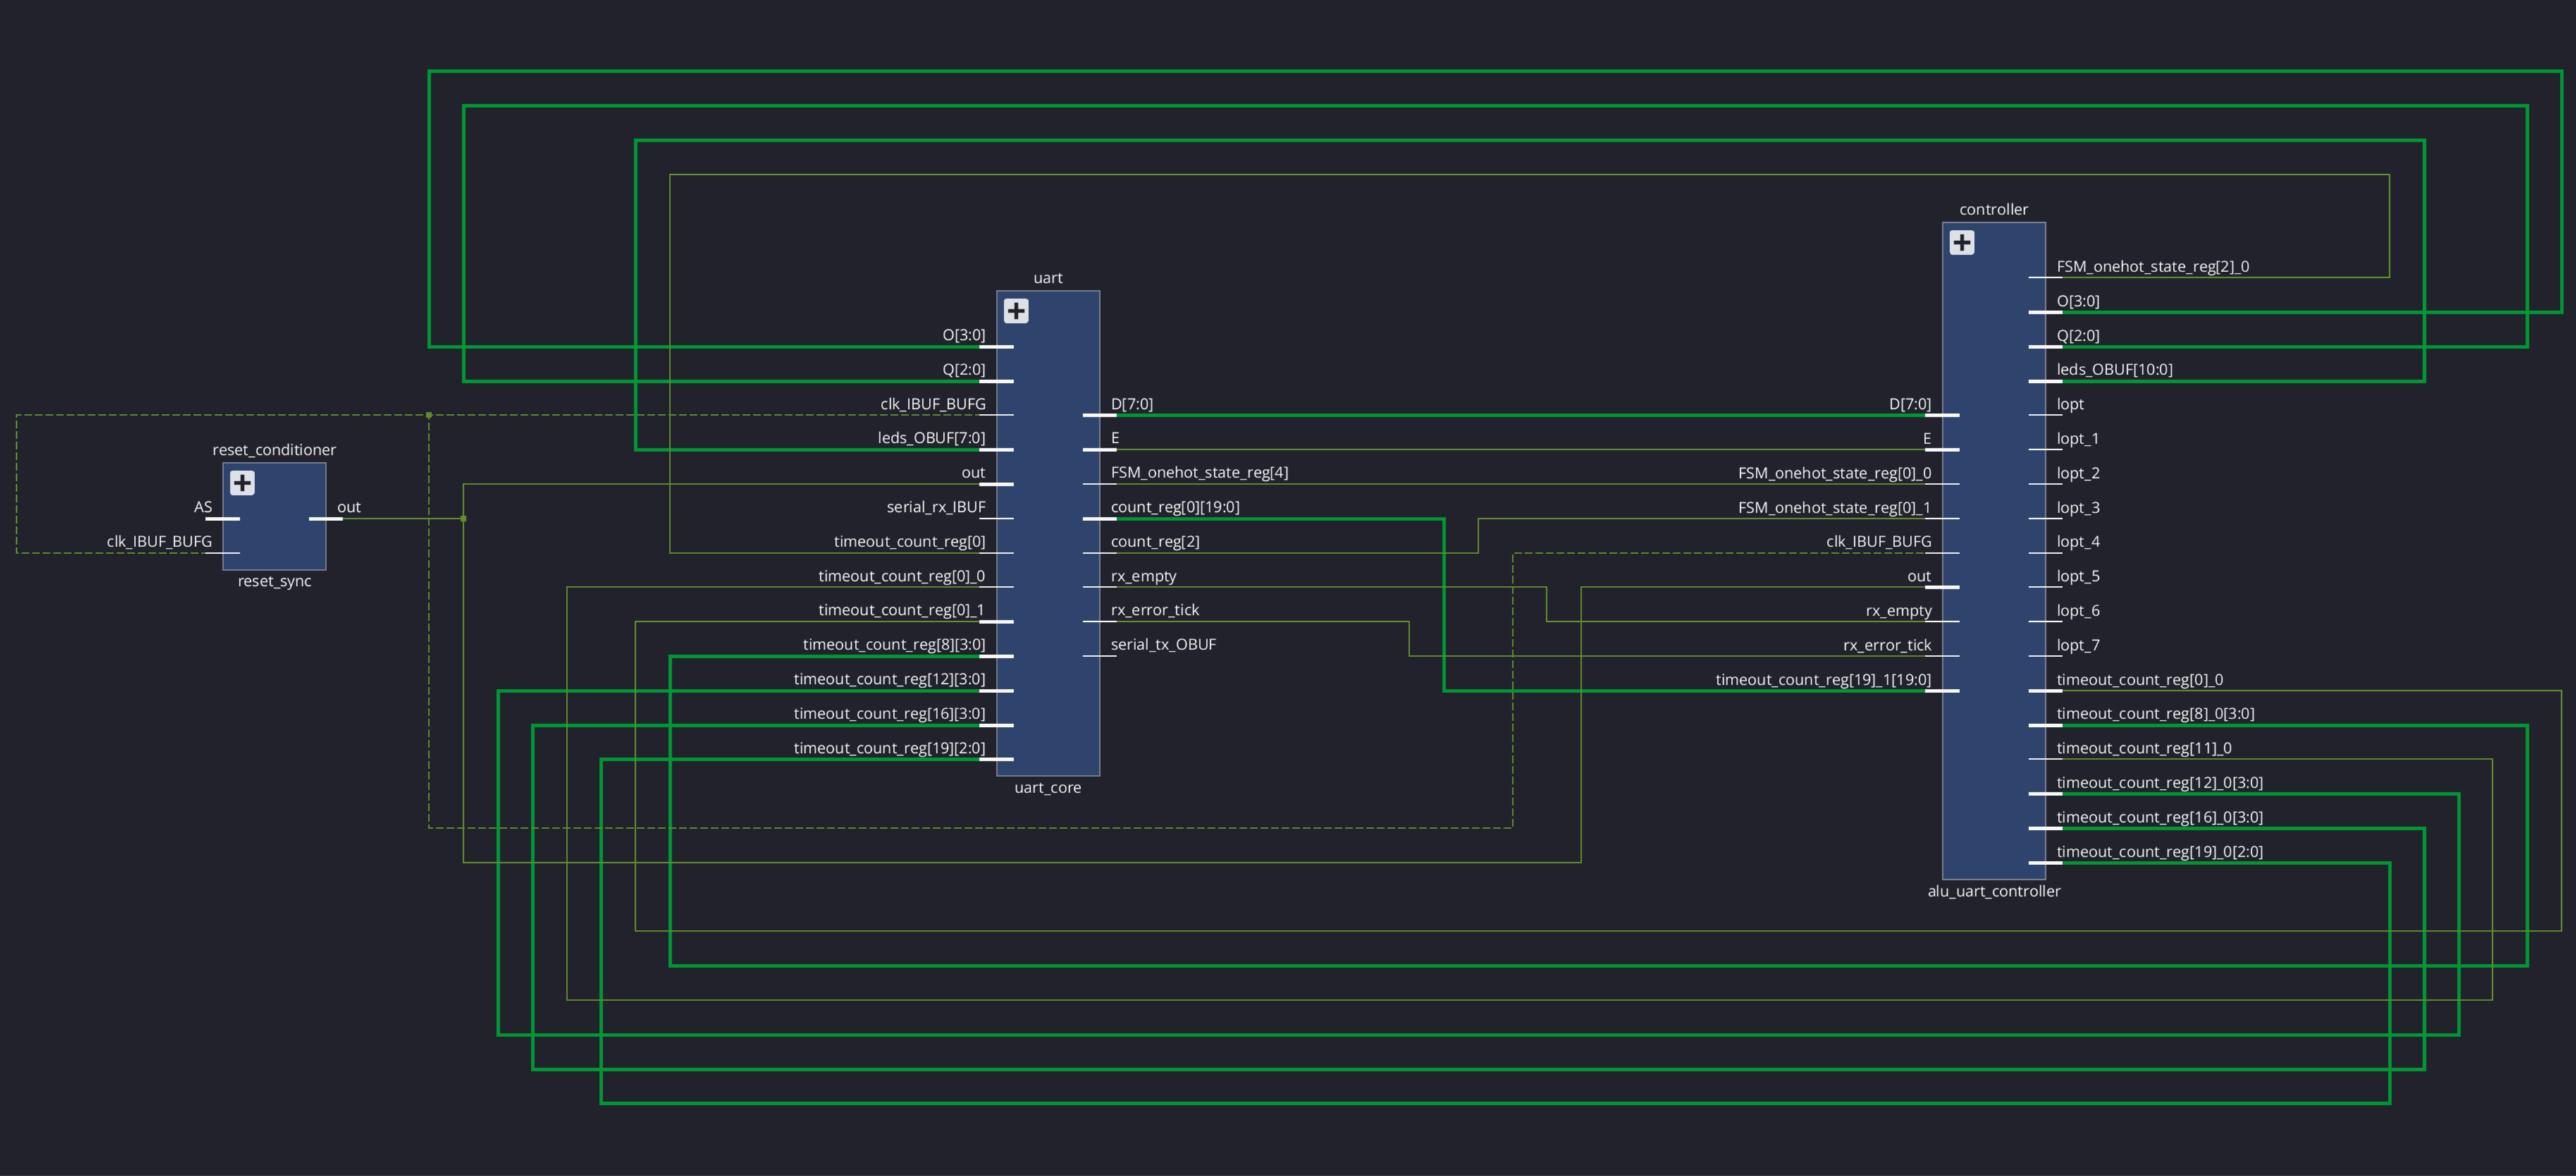
\includegraphics[width=\textwidth]{img/vivado_schematic_top_implementation.png}
  \caption{Esquemático implementado del nivel superior.}%
  \label{fig:schematic-top-implemented}
\end{figure}

Al abrir el núcleo UART se obtiene el esquema de la
figura~\ref{fig:schematic-uart-core-implemented}. En esta vista se
observan los recursos que forman los dos caminos de comunicación y
sus conexiones internas.

\begin{figure}[H]
  \centering
  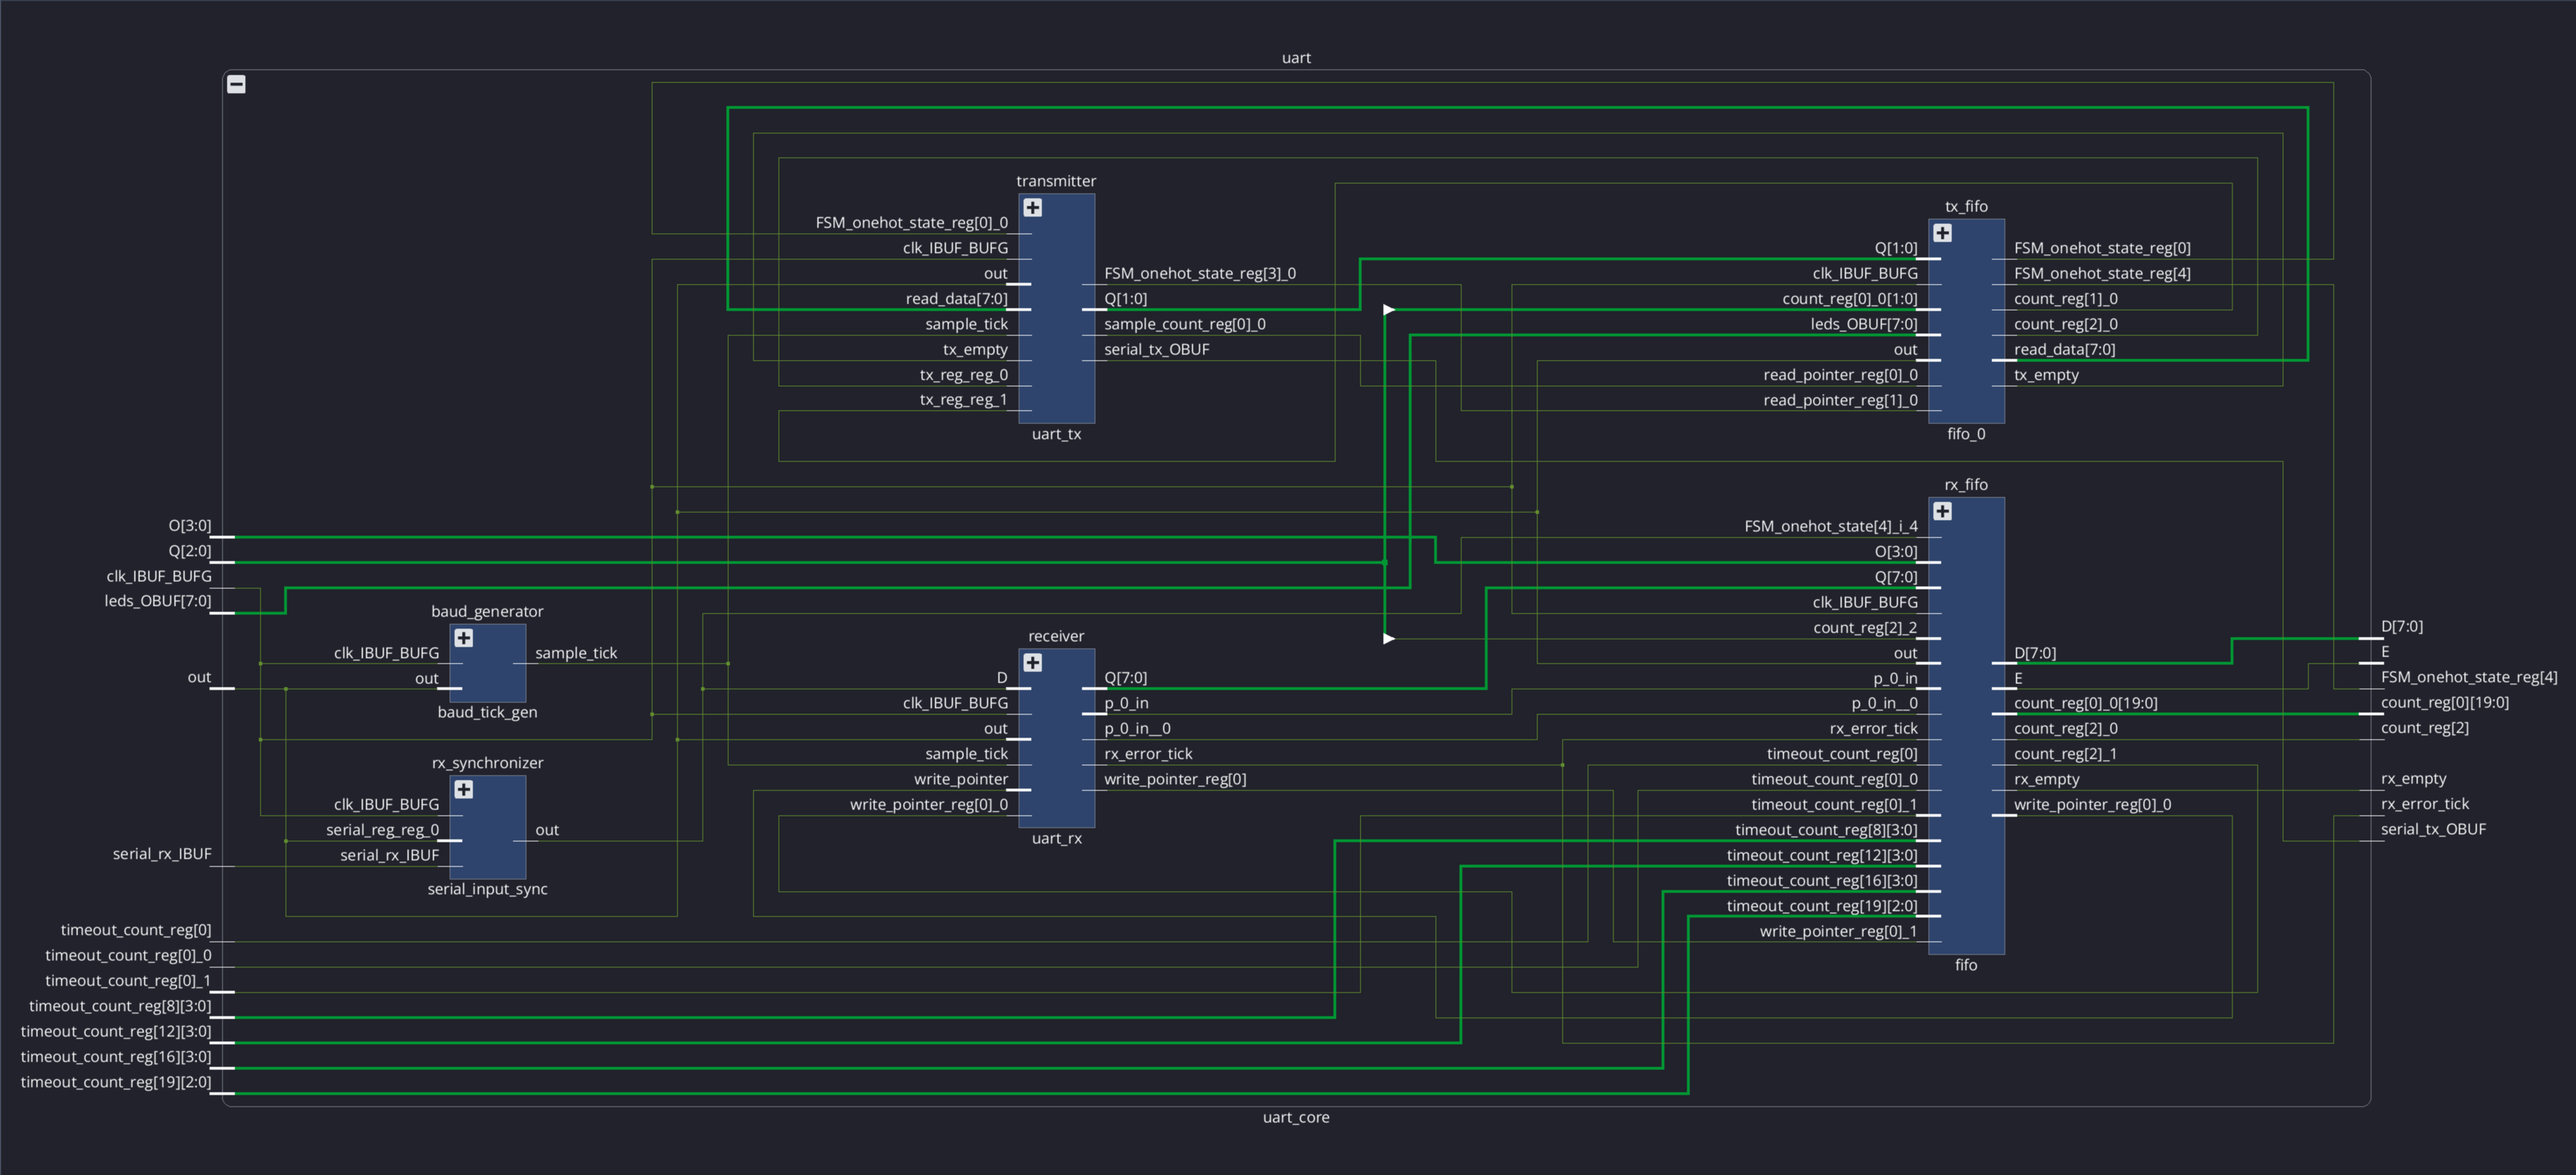
\includegraphics[width=\textwidth]
  {img/vivado_schematic_uart_core_implementation.png}
  \caption{Esquemático implementado del núcleo UART.}%
  \label{fig:schematic-uart-core-implemented}
\end{figure}

La figura~\ref{fig:schematic-controller-implemented} muestra la
implementación del controlador. Los registros que conservan la
transacción y las LUT que determinan las transiciones reemplazan la
representación de mayor nivel observada durante la elaboración.

\begin{figure}[H]
  \centering
  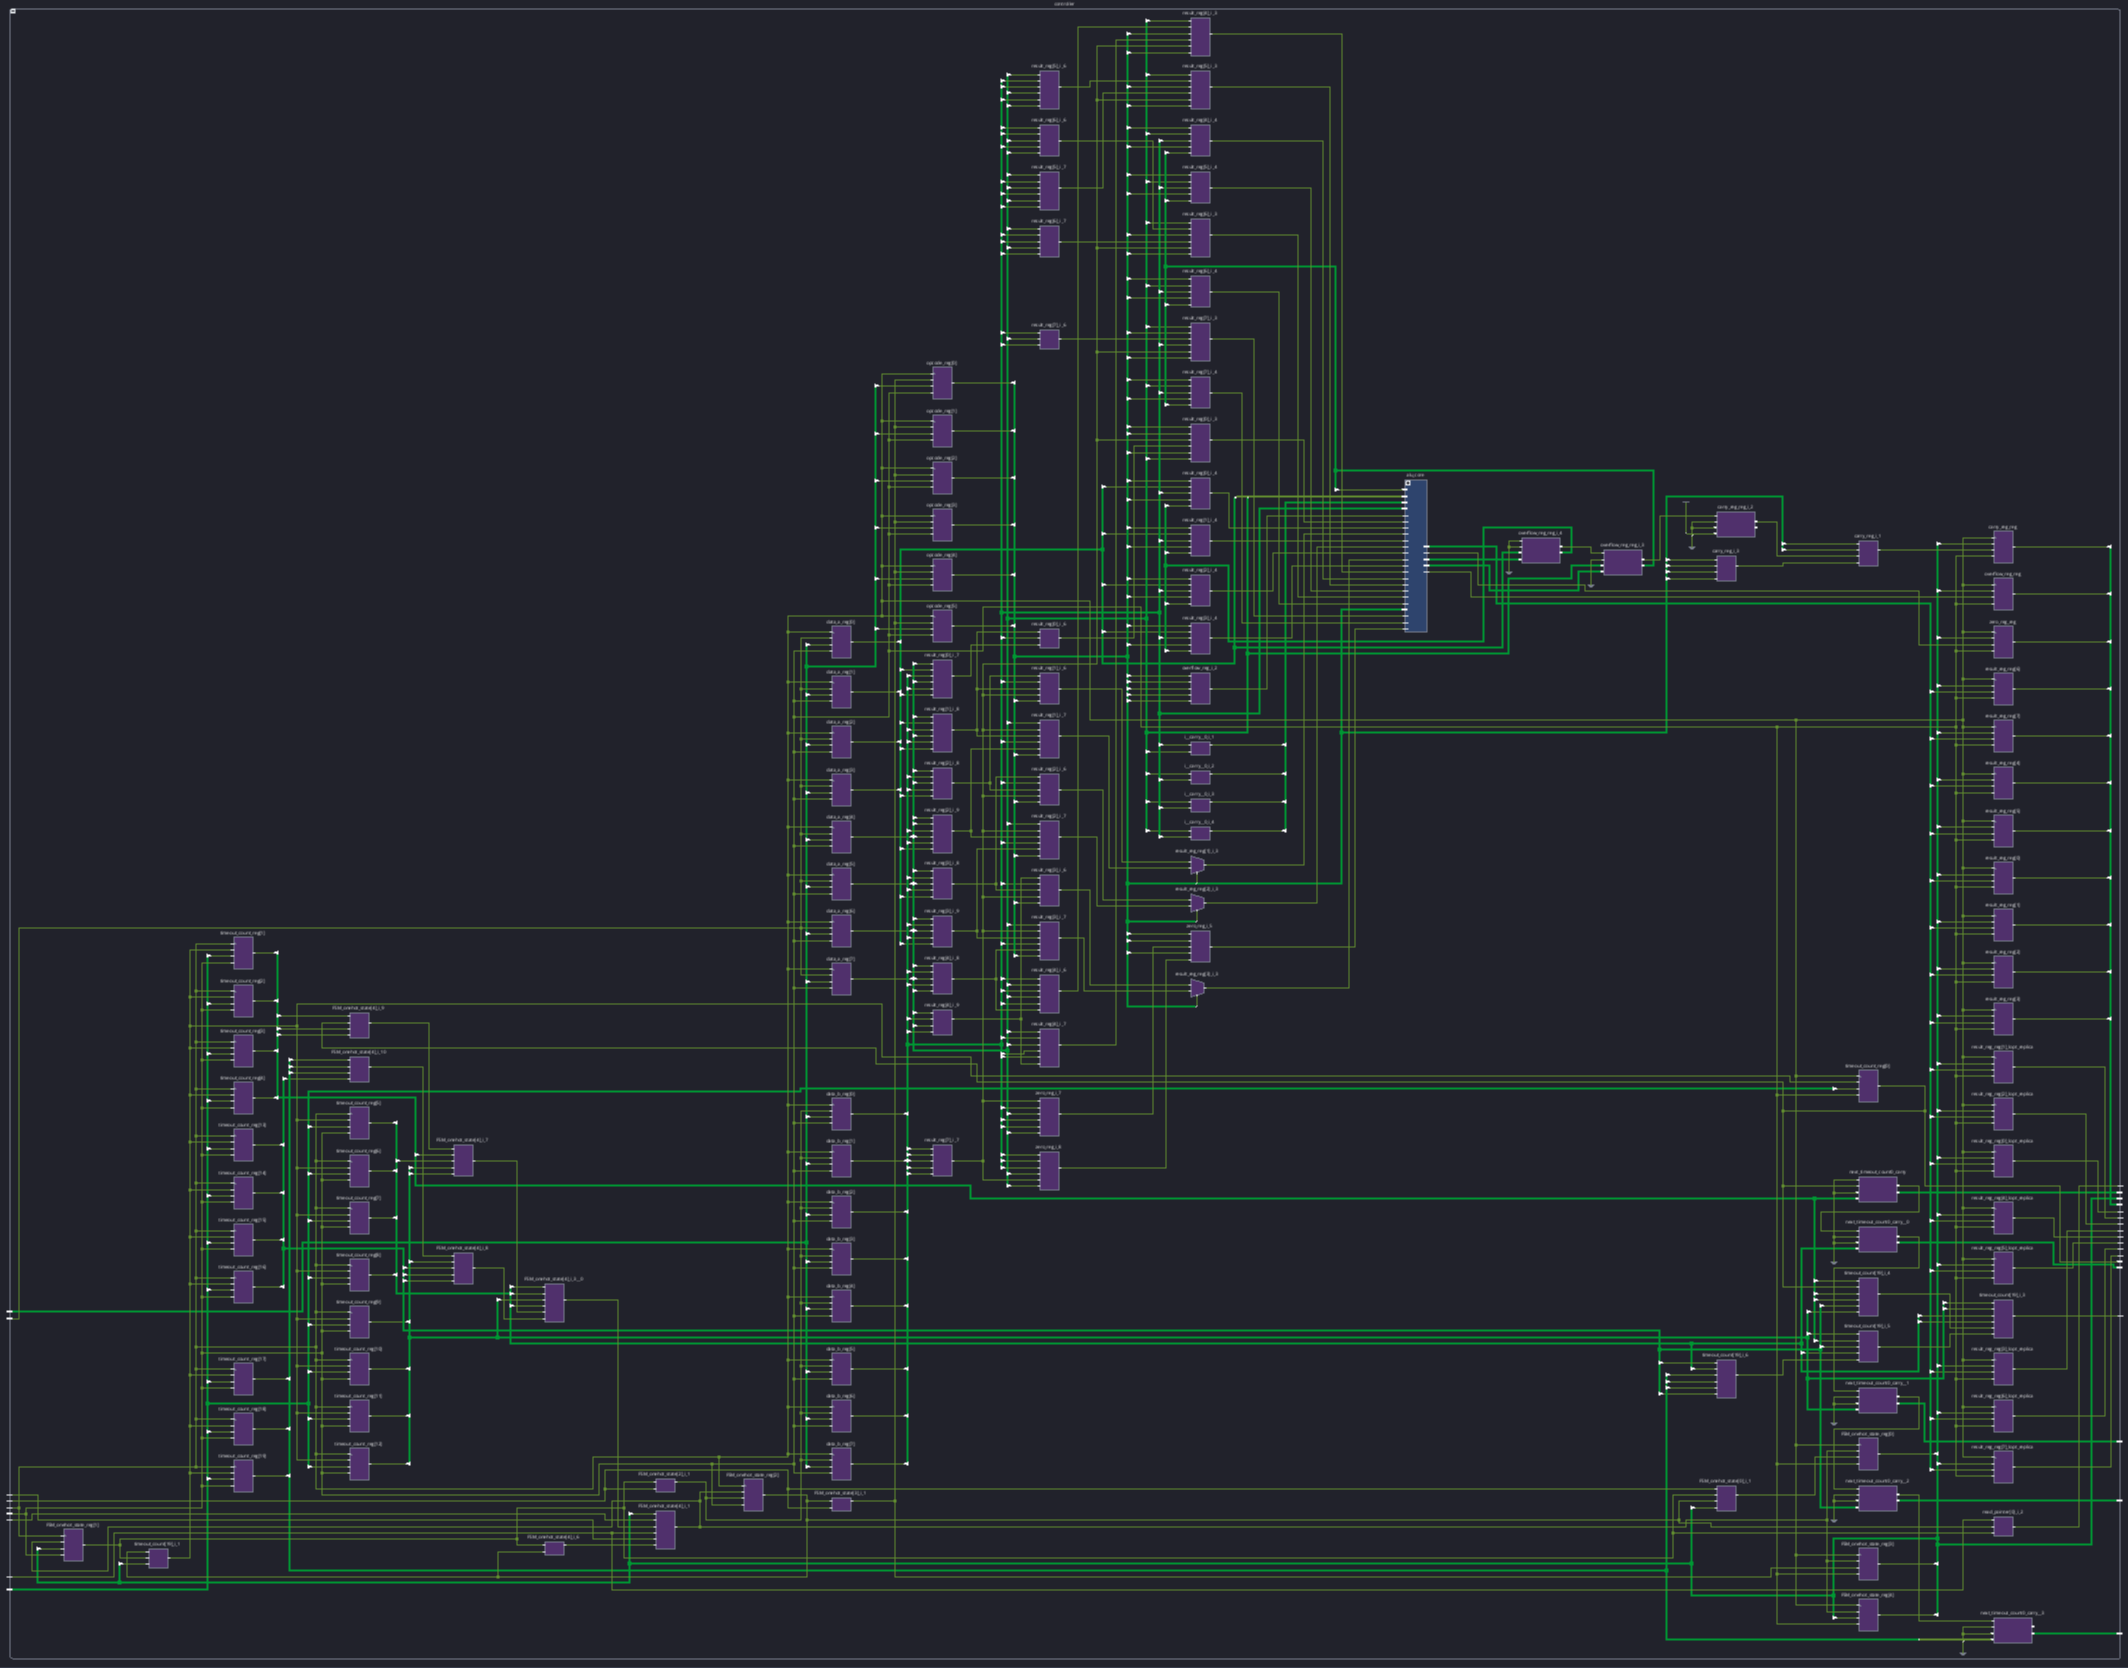
\includegraphics[height=13.0cm,keepaspectratio]
  {img/vivado_schematic_controller_implementation.png}
  \caption{Esquemático implementado del controlador de transacciones.}%
  \label{fig:schematic-controller-implemented}
\end{figure}

Además de los esquemáticos, Vivado permite observar la ubicación de
los recursos sobre el dispositivo. La figura~\ref{fig:device-vivado}
muestra que la lógica ocupa una parte reducida del Artix-7. También
permite comprobar que los pines externos se encuentran en los bancos
indicados por las restricciones de la Basys 3.

\begin{figure}[H]
  \centering
  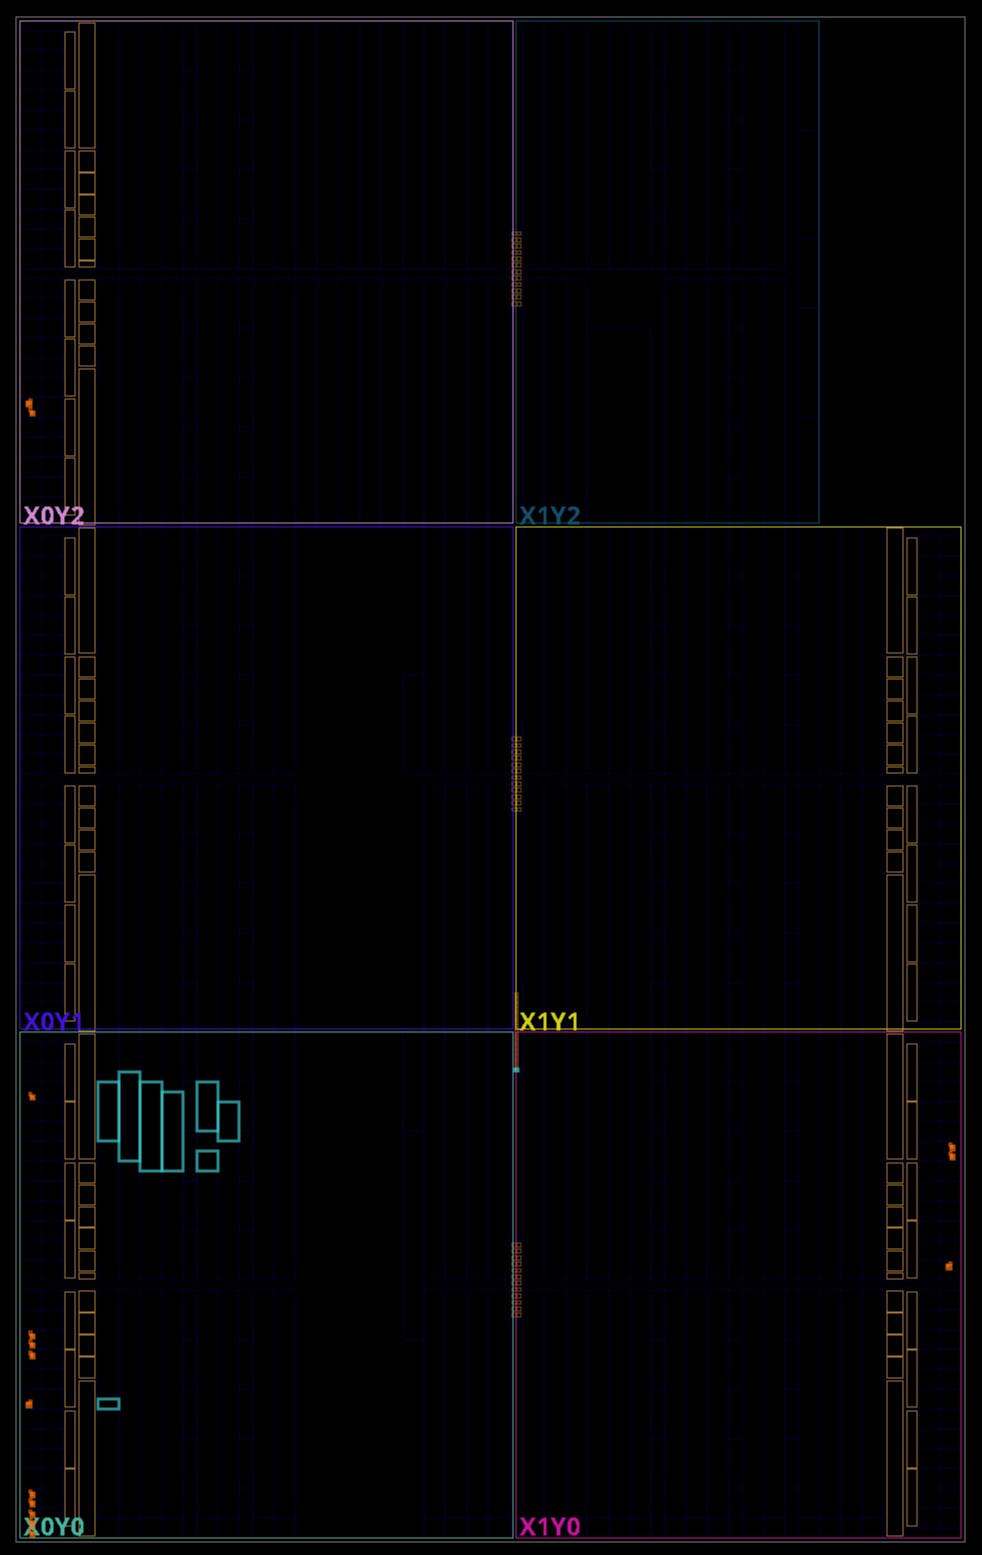
\includegraphics[height=14.5cm,keepaspectratio]{img/vivado_device.png}
  \caption{Vista del dispositivo después de place and route.}%
  \label{fig:device-vivado}
\end{figure}

La tabla~\ref{tab:rtl-recursos} reúne la correspondencia entre los
elementos principales del RTL y los recursos observados después de la
implementación.

\begin{table}[H]
  \centering
  \begin{tabularx}{\textwidth}{L{3.5cm}L{4.1cm}Y}
    \toprule
    \textbf{Elemento RTL} & \textbf{Recurso esperado} & \textbf{Observado} \\
    \midrule
    FSM one-hot & Flip-flops y LUT de transición & 14 bits de estado
    dentro de 134 FF. \\
    Dos FIFO $4\times8$ & Memoria distribuida & 12 LUTRAM post-route. \\
    Suma y resta ALU & LUT y carry chain & LUT/MUXF/CARRY4, 0 DSP. \\
    Registros y contadores & Flip-flops & 134 FF, 0 latches. \\
    Reloj de placa & Buffer global & 1 BUFG. \\
    Puertos físicos & IBUF/OBUF e IOB & 15 IOB asignados. \\
    \bottomrule
  \end{tabularx}
  \caption{Correspondencia entre la descripción y los recursos implementados.}%
  \label{tab:rtl-recursos}
\end{table}

\section{Utilización de recursos}

La correspondencia anterior explica qué tipo de recurso se utilizó.
Para conocer cuánto espacio ocupa el diseño, se revisaron los
reportes \texttt{reports/synthesis\_utilization\_summary.rpt} y
\texttt{reports/implementation\_utilization\_summary.rpt}. El primero
corresponde a la salida de la síntesis. El segundo contiene los
valores obtenidos después de la colocación y el ruteo.

La figura~\ref{fig:utilization-summary} presenta el resumen posterior
al ruteo. La figura~\ref{fig:utilization-hierarchy} distribuye esos
mismos recursos entre las instancias del diseño.

\begin{figure}[H]
  \centering
  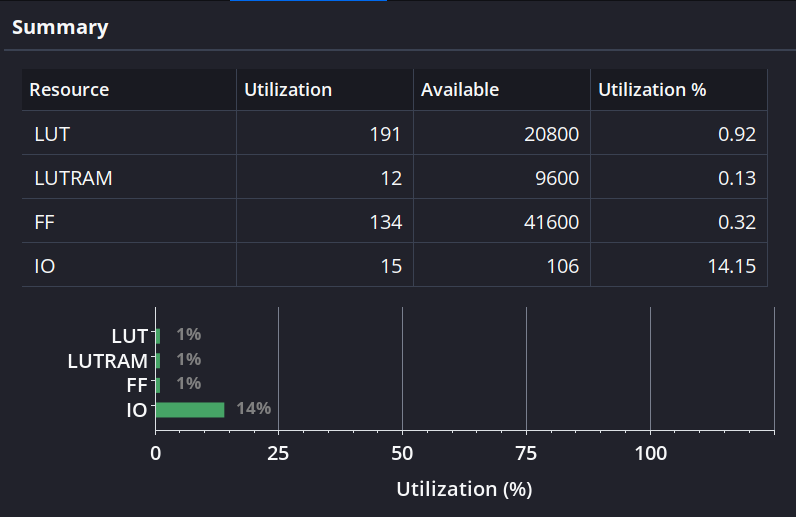
\includegraphics[width=0.65\textwidth]{img/vivado_utilization_summary.png}
  \caption{Resumen de utilización posterior al ruteo.}%
  \label{fig:utilization-summary}
\end{figure}

\begin{figure}[H]
  \centering
  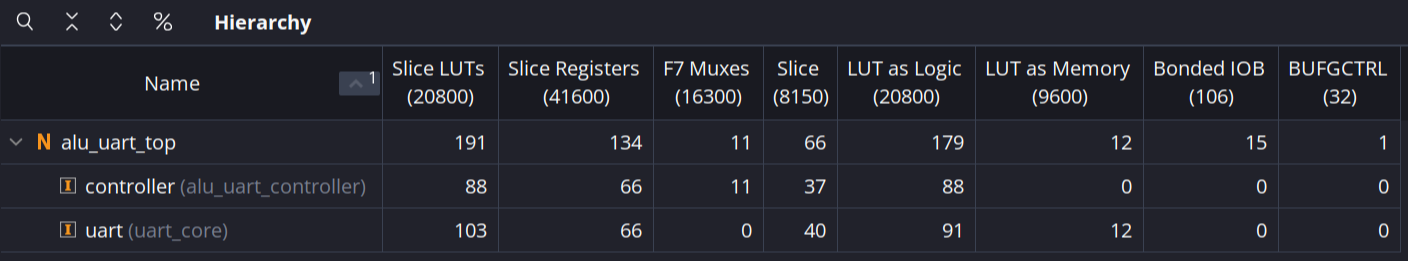
\includegraphics[width=\textwidth]{img/vivado_utilization_hierarchy.png}
  \caption{Distribución jerárquica de los recursos implementados.}%
  \label{fig:utilization-hierarchy}
\end{figure}

Para observar los cambios introducidos durante la implementación, la
tabla~\ref{tab:utilizacion-vivado} compara los valores de síntesis
con los valores posteriores al ruteo.

\begin{table}[H]
  \centering
  \begin{tabularx}{0.88\textwidth}{L{3.2cm}ZZZZ}
    \toprule
    \textbf{Etapa} & \textbf{LUT} & \textbf{LUT lógica} &
    \textbf{LUTRAM} & \textbf{FF} \\
    \midrule
    Síntesis & 197 & 181 & 16 & 126 \\
    Post-route & 191 & 179 & 12 & 134 \\
    Disponible & 20800 & 20800 & 9600 & 41600 \\
    Uso post-route & \SI{0.92}{\percent} & \SI{0.86}{\percent} &
    \SI{0.13}{\percent} & \SI{0.32}{\percent} \\
    \bottomrule
  \end{tabularx}
  \caption{Utilización obtenida antes y después de la implementación.}%
  \label{tab:utilizacion-vivado}
\end{table}

La cantidad total de LUT disminuye de 197 a 191. Dentro de ese total,
las LUT destinadas a lógica pasan de 181 a 179 y las utilizadas como
memoria se reducen de 16 a 12. Estas variaciones se producen durante
las optimizaciones físicas de la implementación.

La cantidad de flip-flops aumenta de 126 a 134. Los ocho registros
adicionales aparecen al adaptar la red sintetizada a los recursos del
dispositivo. Tanto la reducción de LUT como el aumento de registros
son pequeños frente a la capacidad disponible.

El diseño final utiliza 66 slices, 15 de los 106 IOB y uno de los 32
BUFG. No utiliza BRAM ni DSP. La ocupación de LUT y flip-flops
permanece por debajo del uno por ciento. Estos valores muestran que
las dos colas y las tres máquinas de estado poseen un costo reducido
dentro del Artix-7. La ampliación del protocolo queda fuera del
alcance de este trabajo.


\chapter{Timing y limitaciones}
\section{Qué se comprueba}

Después de ubicar y rutear el diseño, es necesario comprobar que la
lógica pueda funcionar con el reloj de la Basys 3. El análisis
temporal estudia los caminos que conectan los registros. Para cada
uno determina si el dato producido por un registro llega a tiempo al
siguiente y permanece estable durante el intervalo necesario.

La comprobación de setup considera el tiempo anterior al flanco de
captura. El dato debe llegar y estabilizarse antes de ese flanco. La
comprobación de hold analiza el intervalo posterior y verifica que el
dato no cambie demasiado pronto. El análisis de ancho de pulso
comprueba que los niveles alto y bajo del reloj duren el tiempo
requerido por el dispositivo.

Cada camino termina en un punto de captura que el reporte denomina
\emph{endpoint}. El margen indica cuánto tiempo queda entre la
llegada del dato y el límite correspondiente a ese punto.

Vivado informa el resultado de setup mediante WNS y TNS. El WNS
corresponde al menor margen encontrado entre todos los caminos. El
TNS suma únicamente los márgenes negativos.

Para hold, el WHS representa el menor margen y el THS reúne los
márgenes negativos. En el análisis del ancho de pulso, el WPWS indica
el peor margen y el TPWS suma las violaciones.

Un valor positivo de WNS o WHS indica que incluso el peor camino
analizado cumple con la restricción. Cuando TNS o THS valen cero, no
existen endpoints con margen negativo. Esto no significa que los
caminos tengan un retardo nulo. Significa que ninguno supera el
límite establecido.

El reloj se define en el archivo \texttt{basys3.xdc}. La restricción
crea \texttt{sys\_clk} con un período de \SI{10}{\nano\second}, que
corresponde a una frecuencia de \SI{100}{\mega\hertz}. A partir de
esta definición, Vivado analiza los caminos internos que comienzan y
terminan en registros controlados por ese reloj.

No todas las señales externas pueden analizarse con la misma relación
temporal. Las entradas {\color{technicalviolet}\path{btn_reset}} y
{\color{technicalviolet}\path{serial_rx}} pueden cambiar sin estar
sincronizadas con {\color{technicalviolet}\path{sys_clk}}. Por eso,
el archivo \texttt{basys3.xdc} declara una excepción desde ambos
puertos hasta la primera etapa de sus sincronizadores mediante
\texttt{set\_false\_path}.

Las doce salidas tampoco poseen una relación temporal con un reloj
externo. Una corresponde a \texttt{serial\_tx} y las otras once
controlan los LED. Como no existe un reloj de captura externo
asociado con \texttt{sys\_clk}, sus caminos hasta los pines también
se declaran con \texttt{set\_false\_path}.

Además de calcular los márgenes, el reporte revisa que la definición
temporal no deje partes internas del diseño sin analizar. El
resultado no presenta registros sin reloj, relojes constantes, lazos
combinacionales ni endpoints internos sin restricción.

El análisis temporal se limita a estas propiedades. No determina si
el protocolo UART interpreta correctamente una solicitud ni si el
enlace USB funciona sobre la placa. El comportamiento del protocolo
se comprobó mediante la simulación funcional. La conexión física se
evalúa en la validación sobre la Basys 3.

\section{Resultado posterior al ruteo}

Una vez definidas las restricciones, el análisis se ejecutó sobre el
diseño completamente ruteado. El archivo
\texttt{reports/timing\_summary.rpt} contiene los resultados
obtenidos para el dispositivo y la velocidad seleccionados.

\subsection{Márgenes temporales}

El reporte incluye 458 endpoints para las comprobaciones de setup y
hold. También analiza 159 endpoints para el ancho de pulso. La
figura~\ref{fig:timing-summary-vivado} muestra el resumen generado
por Vivado. Todos los márgenes son no negativos y las sumas de las
violaciones permanecen en cero.

\begin{figure}[H]
  \centering
  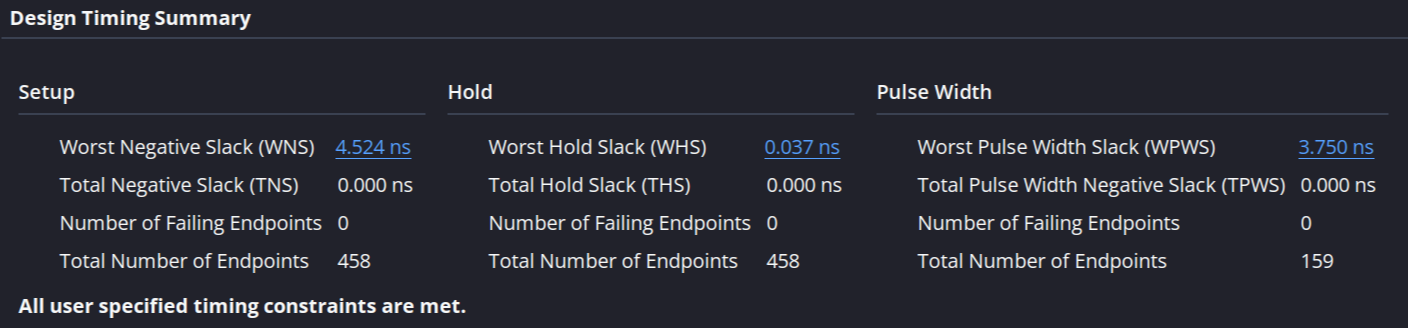
\includegraphics[width=\textwidth]{img/vivado_timing_summary.png}
  \caption{Resumen temporal del diseño posterior al ruteo.}%
  \label{fig:timing-summary-vivado}
\end{figure}

La tabla~\ref{tab:timing} reúne los valores correspondientes a los
tres tipos de análisis.

\begin{table}[H]
  \centering
  \begin{tabularx}{0.92\textwidth}{ZZZZ}
    \toprule
    \textbf{Análisis} & \textbf{Peor margen} & \textbf{Suma negativa} &
    \textbf{Endpoints} \\
    \midrule
    Setup & WNS = \SI{4.524}{\nano\second} & TNS = \SI{0}{\nano\second} & 458 \\
    Hold & WHS = \SI{0.037}{\nano\second} & THS = \SI{0}{\nano\second} & 458 \\
    Ancho de pulso & WPWS = \SI{3.750}{\nano\second} &
    TPWS = \SI{0}{\nano\second} & 159 \\
    \bottomrule
  \end{tabularx}
  \caption{Márgenes reportados después del ruteo.}%
  \label{tab:timing}
\end{table}

El peor camino de setup conserva un margen de
\SI{4.524}{\nano\second} dentro del período de \SI{10}{\nano\second}.
Esto significa que el dato llega con más de cuatro nanosegundos
disponibles antes del límite de captura.

El margen de hold es menor y alcanza \SI{0.037}{\nano\second}. Aun
así, permanece por encima de cero dentro del modelo temporal del
dispositivo. Por esta razón, el THS es igual a cero y no se informan
endpoints con una violación de hold. El análisis del ancho de pulso
también cumple, con un WPWS de \SI{3.750}{\nano\second} y un TPWS igual a cero.

Estos resultados permiten afirmar que el diseño implementado
satisface las restricciones declaradas para un reloj de \SI{100}{\mega\hertz}.

\subsection{Cruces asíncronos}

El análisis de los caminos síncronos no alcanza para evaluar las
señales que ingresan sin relación con el reloj interno. Por ese
motivo también se realizó un análisis CDC, denominado \emph{Clock
Domain Crossing}. Su resultado se guarda en \texttt{reports/cdc.rpt}.
Este análisis comprueba que los cruces entre dominios de reloj
atraviesen las estructuras de sincronización previstas.

El reporte identifica exactamente dos cruces. El primero corresponde
a la liberación del reset y aparece clasificado como CDC-9. El
segundo corresponde a la entrada \texttt{serial\_rx} y aparece como
CDC-3. Ambos sincronizadores tienen una profundidad de dos etapas y
poseen la propiedad \texttt{ASYNC\_REG}. Además, los caminos desde
los puertos externos están cubiertos por las excepciones declaradas
en \texttt{basys3.xdc}. El reporte identifica ambas excepciones como
\texttt{False Path}.

La figura~\ref{fig:cdc-vivado} muestra ambos cruces y permite
comprobar su clasificación, su profundidad y la excepción aplicada.

\begin{figure}[H]
  \centering
  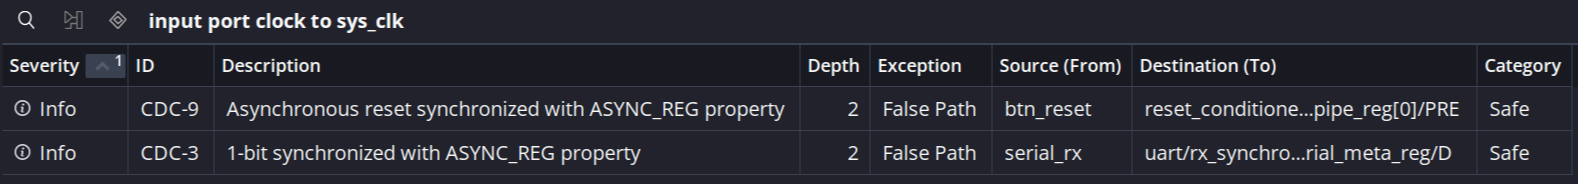
\includegraphics[width=\textwidth]{img/vivado_cdc.png}
  \caption{Cruces de dominio identificados por el análisis CDC.}%
  \label{fig:cdc-vivado}
\end{figure}

\subsection{DRC y metodología}

Después de revisar la temporización y los cruces asíncronos, se
ejecutó el DRC, o \emph{Design Rule Check}. Esta comprobación revisa
las reglas del dispositivo sobre el diseño completamente ruteado. El
archivo \texttt{reports/drc.rpt} informa \texttt{Checks found: 0}.
Por lo tanto, no se encontró ninguna violación.

La figura~\ref{fig:drc-vivado} presenta el resumen de esta comprobación.

\begin{figure}[H]
  \centering
  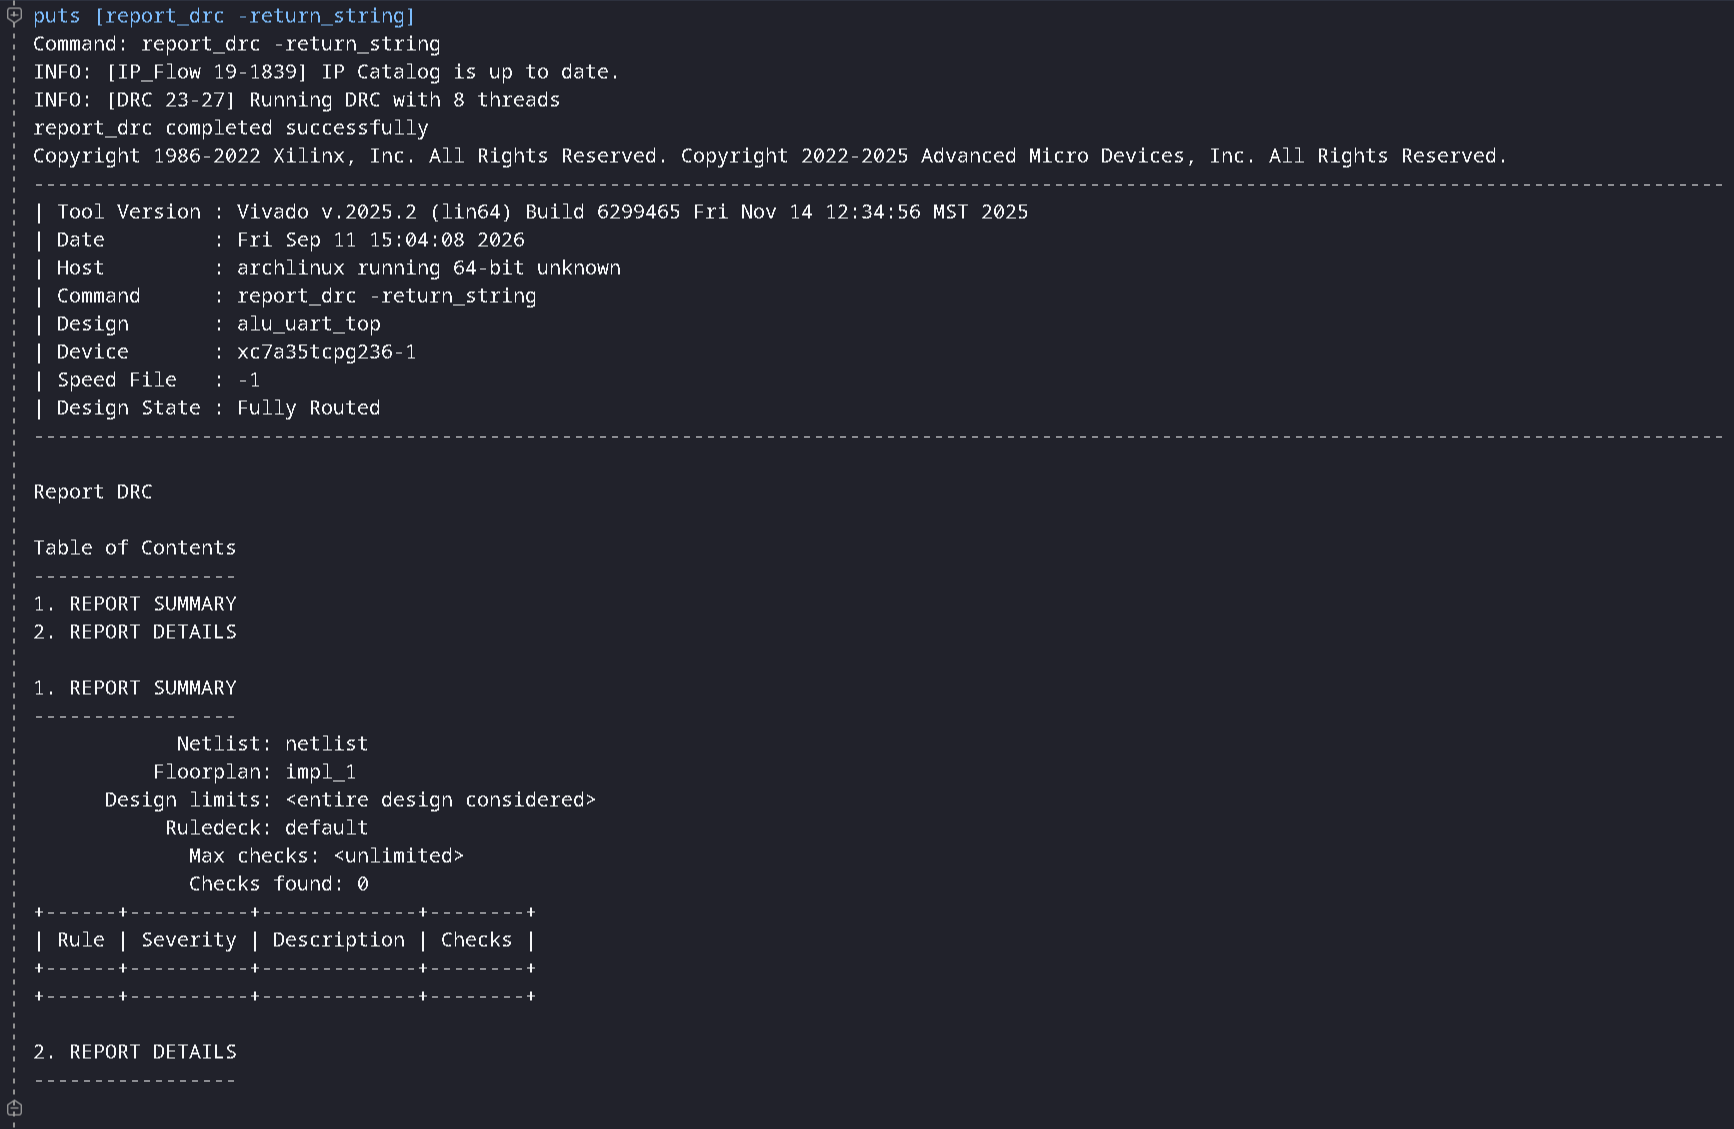
\includegraphics[width=0.72\textwidth]{img/vivado_drc.png}
  \caption{DRC del diseño completamente ruteado, sin violaciones.}%
  \label{fig:drc-vivado}
\end{figure}

Los reportes de metodología revisan otro aspecto del proceso. En este
caso, Vivado busca construcciones o decisiones que no respeten sus
re\-co\-men\-da\-cio\-nes para la síntesis y la
im\-ple\-men\-ta\-ción. El archivo
\texttt{reports/synthesis\allowbreak\_methodology.rpt} no contiene
hallazgos después de la síntesis. El archivo
\texttt{reports/implementation\allowbreak\_methodology.rpt} tampoco
presenta hallazgos después de completar la implementación.

Las figuras~\ref{fig:methodology-synthesis-vivado} y
\ref{fig:methodology-implementation-vivado} muestran los resúmenes de
ambos reportes.

Las capturas permiten observar los resultados principales, pero los
reportes conservan el detalle completo de cada análisis. Los archivos
utilizados son
{\color{technicalviolet}\path{reports/timing_summary.rpt}},
{\color{technicalviolet}\path{reports/cdc.rpt}},
{\color{technicalviolet}\path{reports/drc.rpt}},
{\color{technicalviolet}\path{reports/synthesis_methodology.rpt}} y
{\color{technicalviolet}\path{reports/implementation_methodology.rpt}}.

\clearpage

\begin{figure}[H]
  \centering
  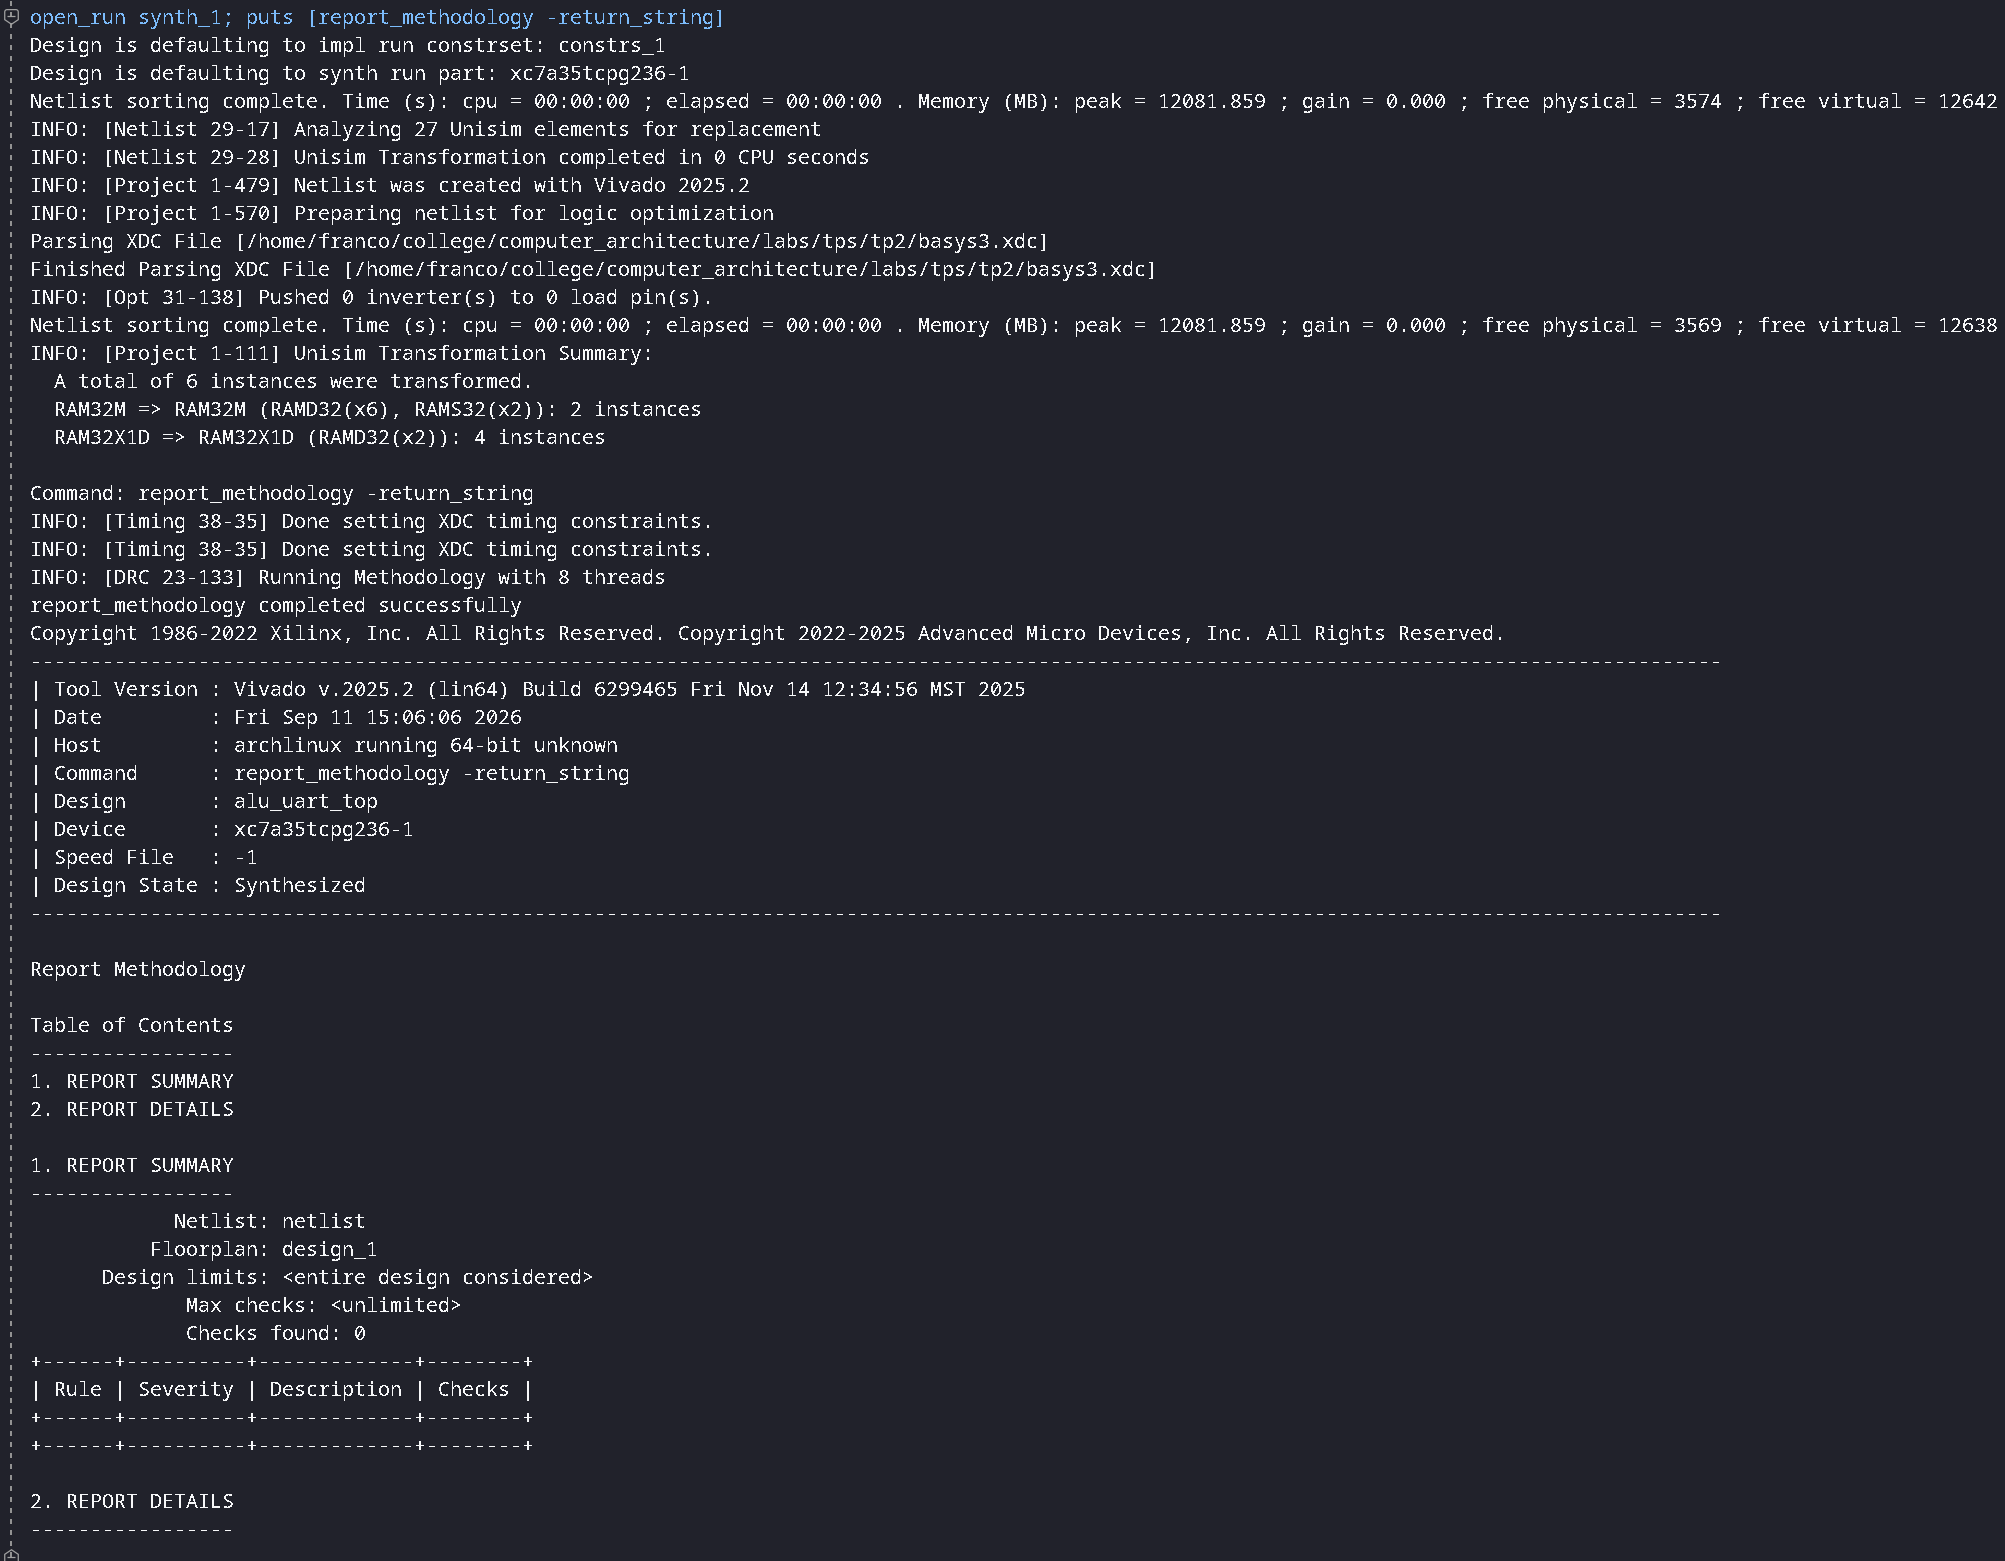
\includegraphics[width=0.74\textwidth]
  {img/vivado_methodology_synthesis.png}
  \caption{Reporte de metodología posterior a síntesis, sin hallazgos.}%
  \label{fig:methodology-synthesis-vivado}
\end{figure}

\begin{figure}[H]
  \centering
  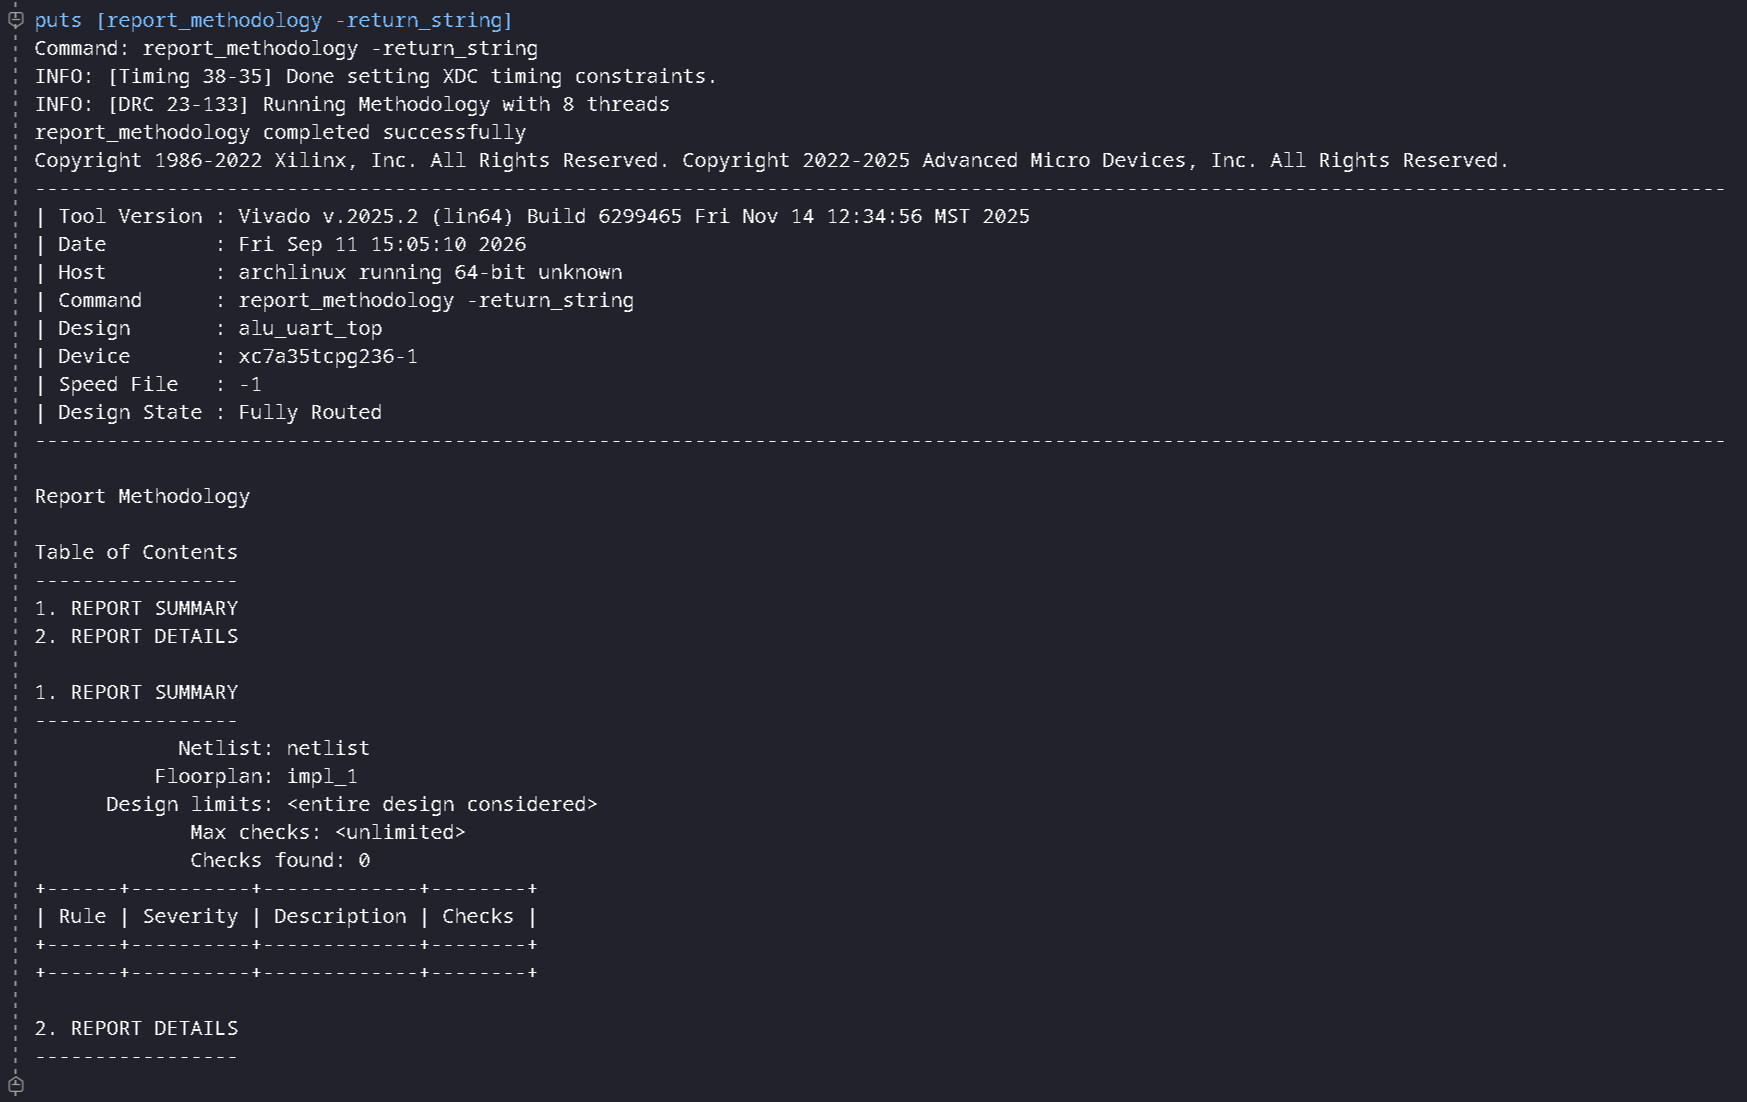
\includegraphics[width=0.82\textwidth]
  {img/vivado_methodology_implementation.png}
  \caption{Reporte de metodología posterior a implementación, sin hallazgos.}%
  \label{fig:methodology-implementation-vivado}
\end{figure}


\chapter{Validación física}\label{chap:validacion}
\section{Objetivo y montaje}

La validación física comprobó el funcionamiento del sistema completo sobre una
Basys 3. A diferencia de la simulación y del análisis posterior al ruteo, este
ensayo incluyó el cable Micro-USB, la interfaz JTAG, el puente USB--UART, el
oscilador de la placa y los LED utilizados como salida. El recorrido observado
comenzó en la interfaz gráfica de la computadora, atravesó el enlace serie y la
ALU implementada en la FPGA, y terminó tanto en la respuesta UART como en los
indicadores de la placa.

Con la placa apagada, el selector de alimentación se colocó en USB y el cable
Micro-USB se conectó a J4, identificado como \texttt{PROG}. Luego se accionó
SW16 y se comprobó el encendido de LD20. El mismo enlace proporcionó
alimentación, acceso JTAG y comunicación USB--UART, tal como se describe en el
\href{https://digilent.com/reference/_media/reference/programmable-logic/basys-3/basys3_rm.pdf}{manual de referencia de la Basys 3}.

\section{Programación y conexión}

El proyecto \texttt{vivado/tp2\_uart/tp2\_uart.xpr} se abrió en Vivado y se
estableció la conexión desde \textit{Open Hardware Manager} mediante
\textit{Open Target $\rightarrow$ Auto Connect}. Hardware Manager detectó el
dispositivo \texttt{xc7a35t\_0}, sobre el cual se cargó
\texttt{build/alu\_uart\_top.bit} con \textit{Program Device}. La
figura~\ref{fig:hardware-manager-placa} muestra el dispositivo en estado
\textit{Programmed}. El LED \texttt{DONE} de la placa permaneció encendido
durante los ensayos.

\begin{figure}[H]
	\centering
	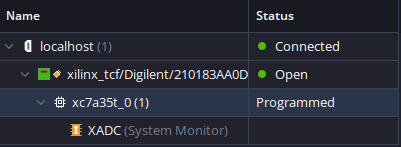
\includegraphics[width=0.60\textwidth]{img/vivado_hardware_manager_placa.png}
	\caption{Basys 3 detectada y programada desde Vivado Hardware Manager.}%
	\label{fig:hardware-manager-placa}
\end{figure}

Después de la programación se presionó y se soltó BTNC para llevar todos los
registros a su estado inicial. Para operar el sistema se inició la aplicación
gráfica desarrollada en Python:

\begin{codebox}
tools/.venv/bin/python tools/uart_alu_gui.py
\end{codebox}

La aplicación enumeró los puertos disponibles y reconoció el puente de
Digilent como \texttt{/dev/ttyUSB1}. Se seleccionaron \num{19200} baud, ocho
bits de datos, sin paridad, un bit de stop y sin control de flujo. Al presionar
\textit{Conectar}, el indicador cambió de \textit{Sin conexión} a
\textit{Conectado}, como se observa en la figura~\ref{fig:gui-conexion}. El
selector de baud configura el extremo de la computadora; no modifica el
bitstream, por lo que debe coincidir con el valor implementado en la FPGA.

\begin{figure}[H]
	\centering
	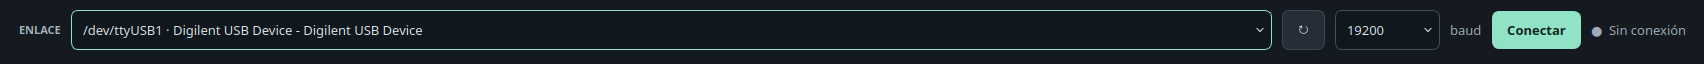
\includegraphics[width=0.98\textwidth]{img/uart_gui_port_selected.png}\par\vspace{0.25cm}
	
\includegraphics[width=0.98\textwidth]{img/uart_gui_connected.png}
	\caption{Selección del puente USB--UART y conexión de la GUI a
	\texttt{/dev/ttyUSB1} a \num{19200} baud.}%
	\label{fig:gui-conexion}
\end{figure}

\section{Pruebas realizadas}

\subsection{Casos dirigidos}

La primera ejecución aplicó los trece casos dirigidos provistos por la vista
\textit{Pruebas}. El conjunto cubrió las ocho operaciones, resultados nulos,
carry, overflow y un opcode inválido. Para cada fila, la aplicación calculó el
valor esperado con el modelo de referencia, envió los tres bytes
A--B--opcode y comparó el único byte recibido desde la placa.

La ejecución finalizó con 13 operaciones completadas, 13 correctas y ninguna
diferencia. La figura~\ref{fig:gui-dirigidos} conserva además los operandos, el
opcode, los valores esperado y recibido, y el tiempo de cada transacción.

\begin{figure}[H]
	\centering
	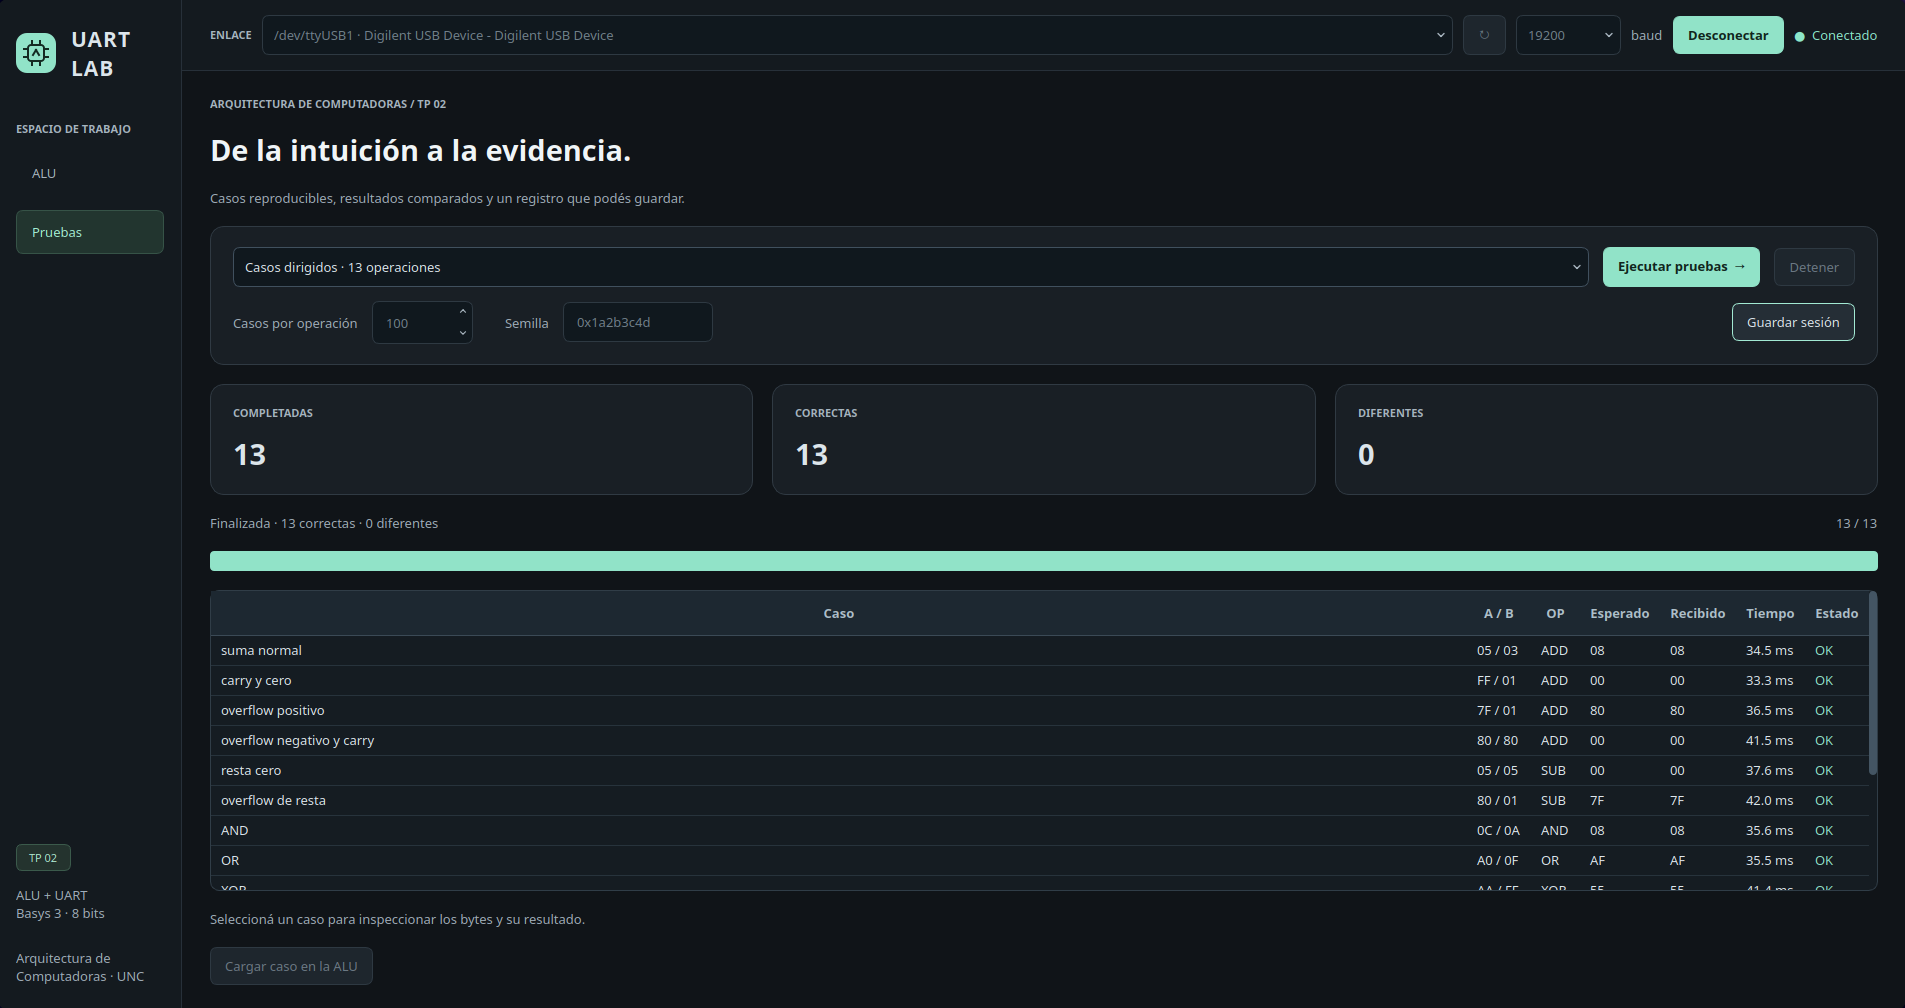
\includegraphics[width=\textwidth]{img/uart_gui_directed.png}
	\caption{Resultado de la suite dirigida ejecutada sobre la Basys 3: 13 de
	13 casos correctos.}%
	\label{fig:gui-dirigidos}
\end{figure}

\subsection{Casos pseudoaleatorios}

La segunda ejecución utilizó cien pares de operandos por cada una de las ocho
operaciones. La semilla \texttt{0x1a2b3c4d} fijó la secuencia y permitió que el
conjunto de 800 transacciones fuera reproducible. La prueba terminó con 800
respuestas correctas y ninguna diferencia respecto del modelo, según la
figura~\ref{fig:gui-aleatorios}.

\begin{figure}[H]
	\centering
	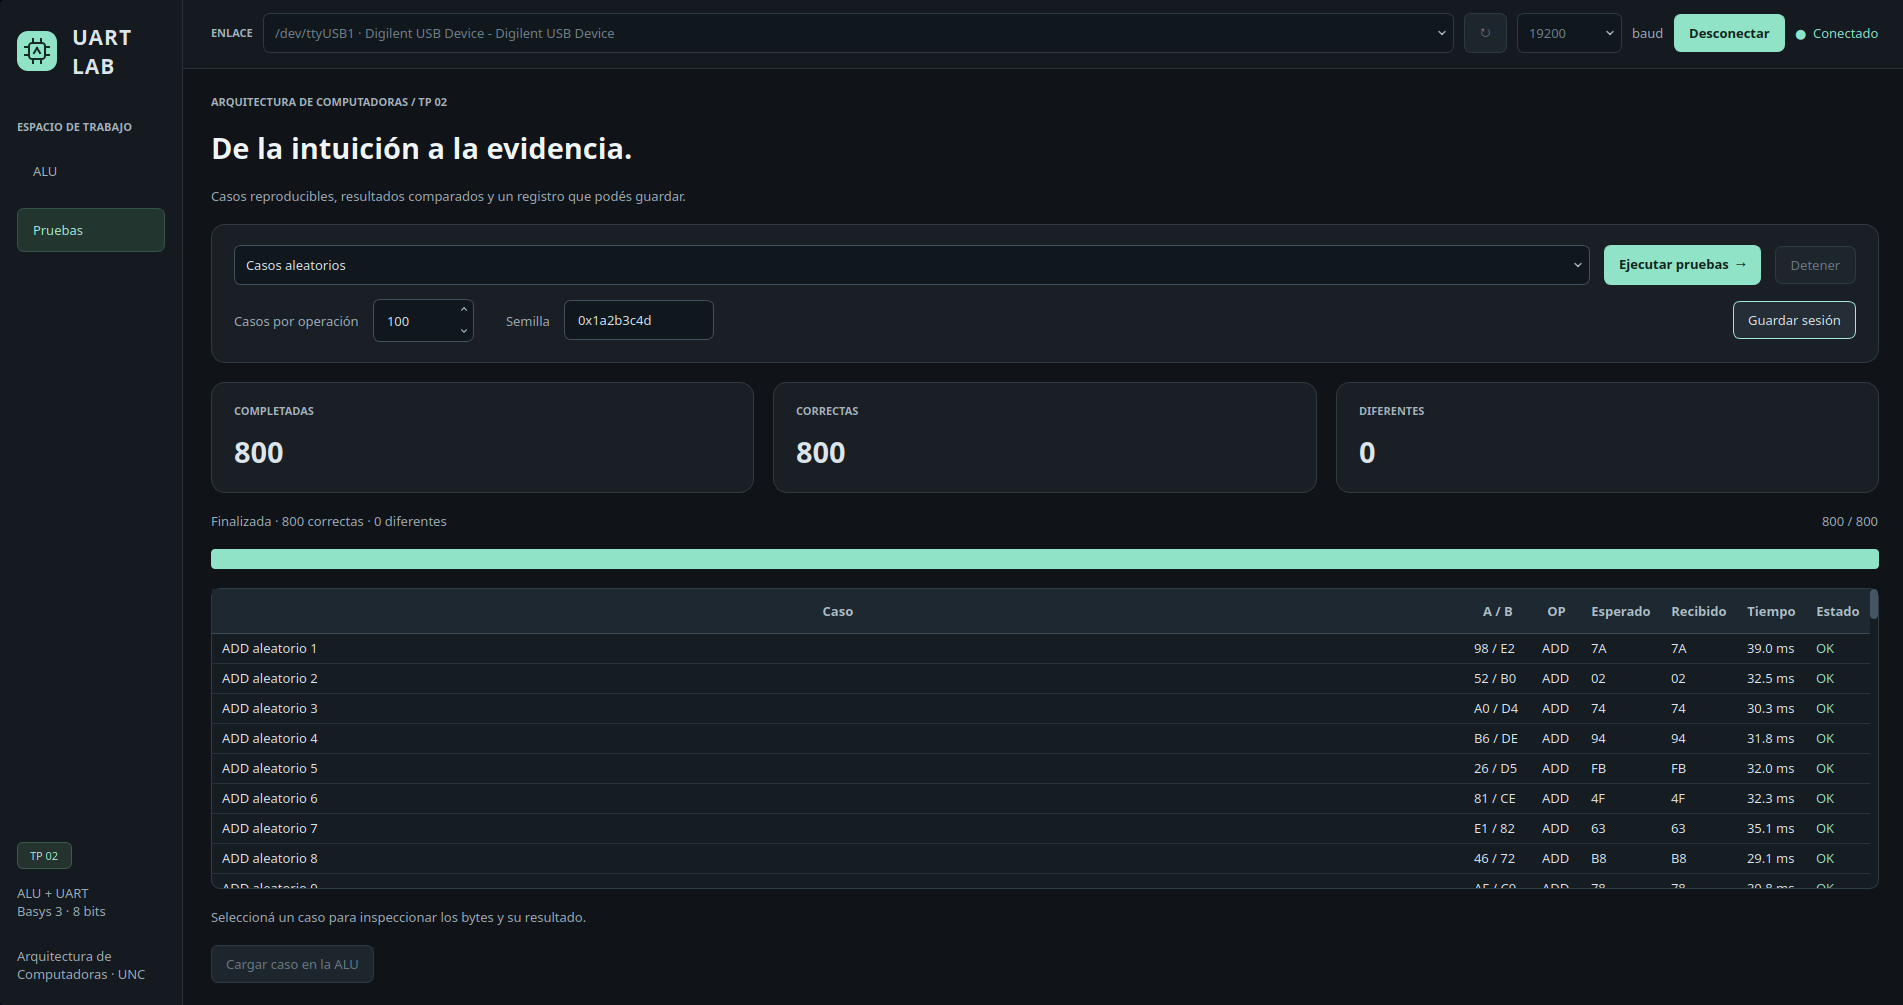
\includegraphics[width=\textwidth]{img/uart_gui_random.png}
	\caption{Resultado de la suite pseudoaleatoria: 800 de 800 respuestas
	coincidentes con el modelo.}%
	\label{fig:gui-aleatorios}
\end{figure}

\subsection{Correspondencia entre UART y LED}

La respuesta UART contiene únicamente el resultado de ocho bits. Las banderas
Z, C y V que presenta la GUI son los valores calculados por el modelo local y
no datos recibidos desde la FPGA. Por esa razón se repitieron manualmente dos
casos de frontera y se comparó la respuesta de la GUI con los LED físicos.

La operación \texttt{FF + 01} produjo la respuesta UART \texttt{00}. En la
GUI, el byte recibido coincidió con el esperado; en la placa quedaron
encendidos LD8 (Z) y LD9 (C), mientras que LD10 (V) y LD0--LD7 permanecieron
apagados. El patrón completo fue, por lo tanto, \texttt{0x300}. La
figura~\ref{fig:validacion-carry-zero} reúne ambas observaciones.

\begin{figure}[H]
	\centering
	\begin{minipage}[c]{0.58\textwidth}
		\centering
		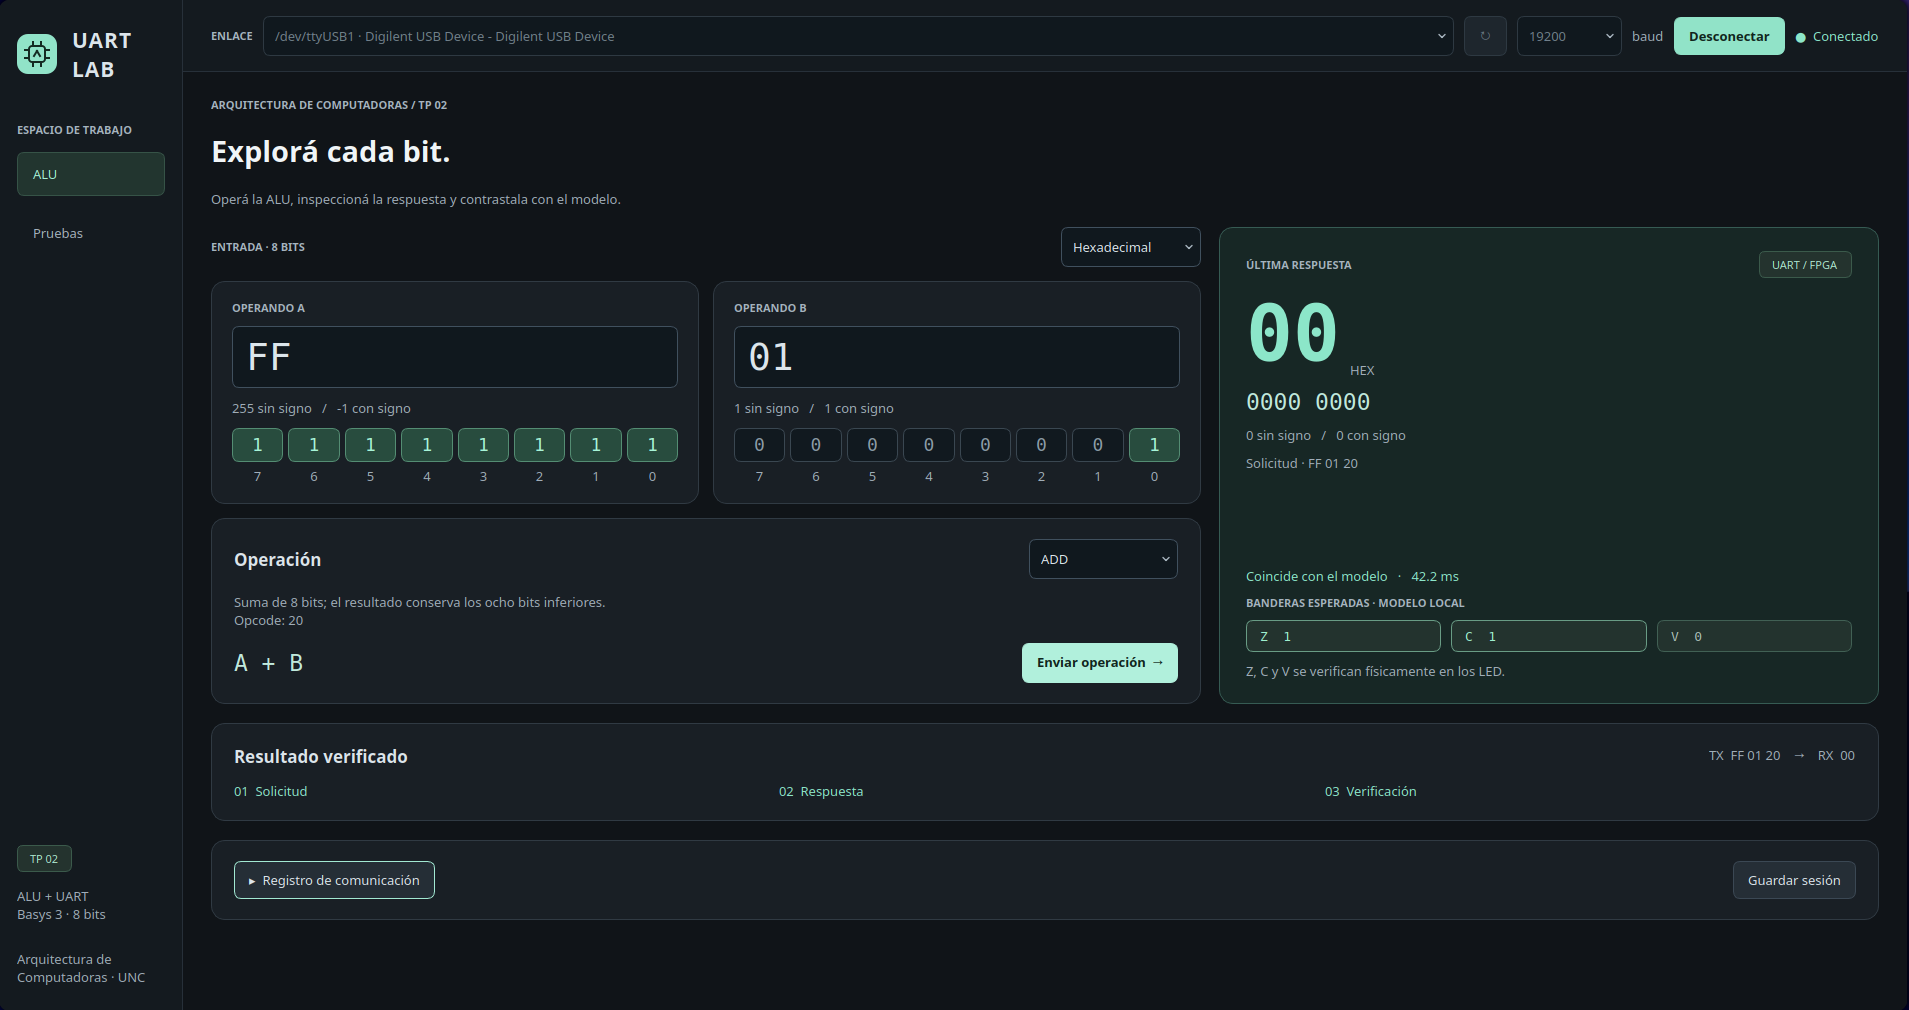
\includegraphics[width=\linewidth]{img/uart_gui_add_ff_01.png}
	\end{minipage}\hfill
	\begin{minipage}[c]{0.38\textwidth}
		\centering
		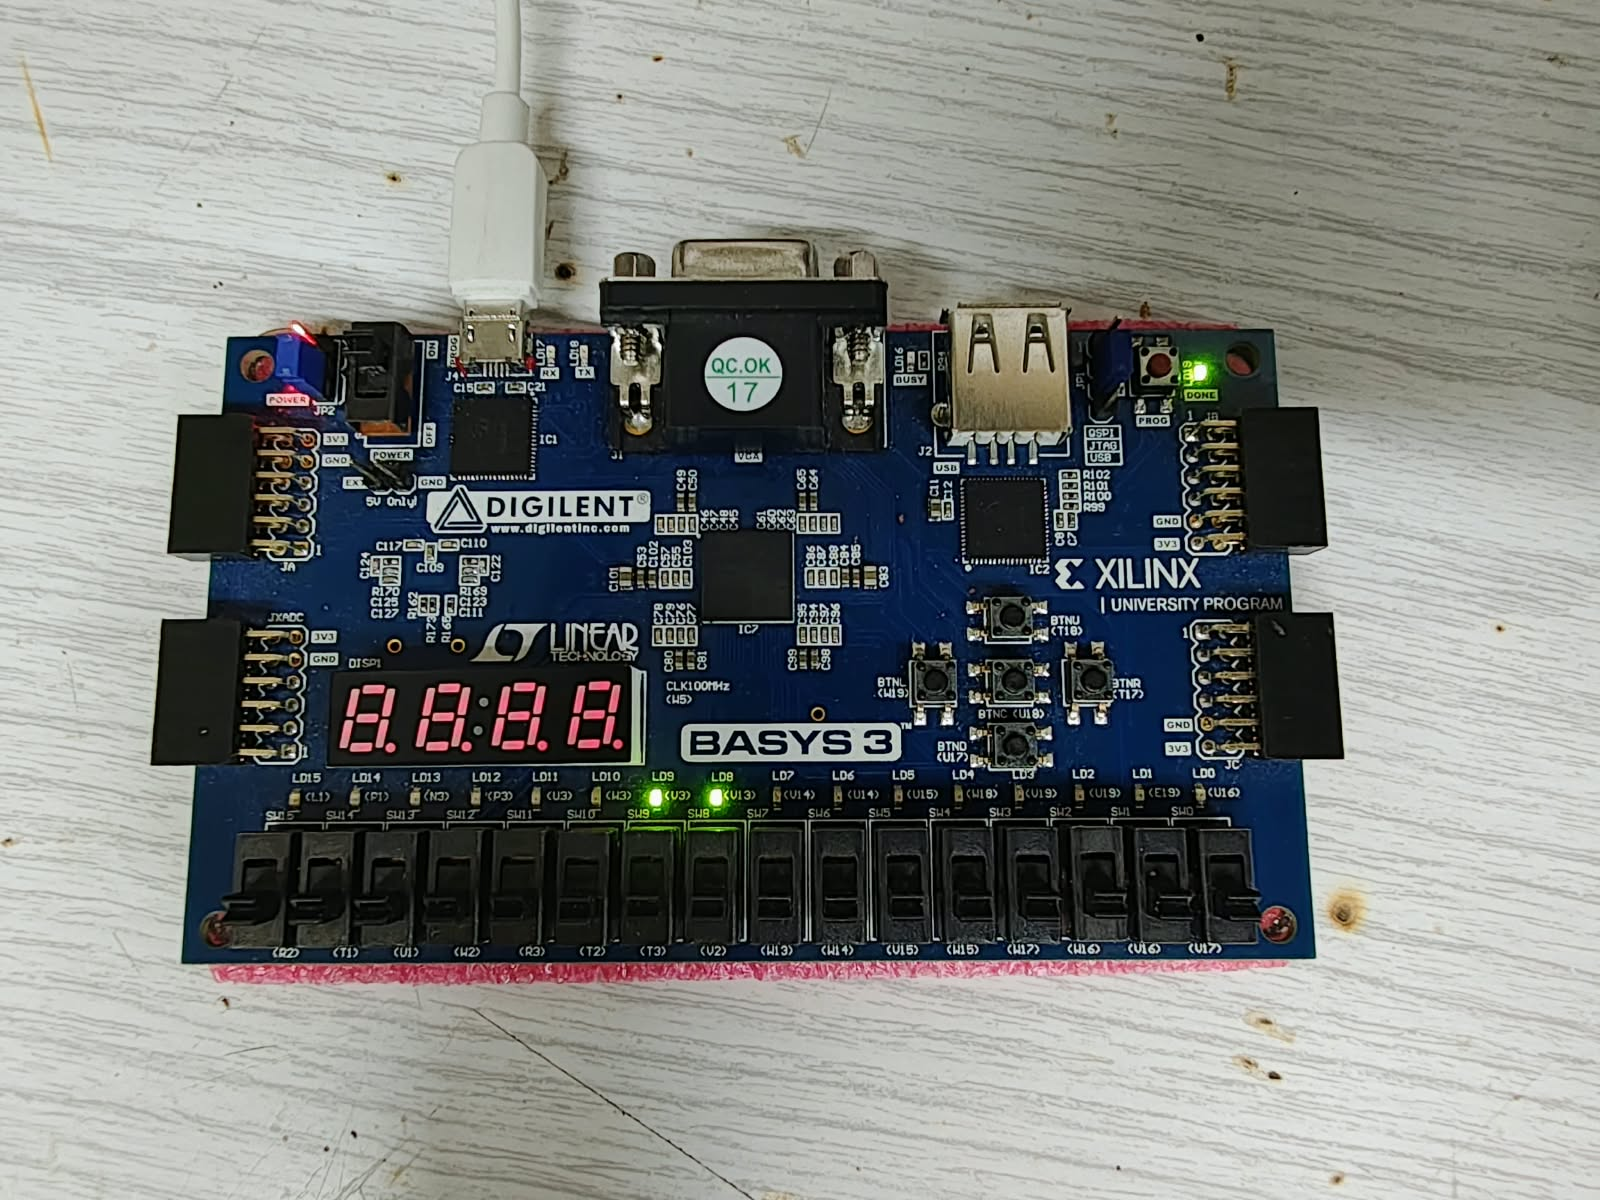
\includegraphics[width=\linewidth]{img/basys3_uart_carry_zero.jpg}
	\end{minipage}
	\caption{Suma \texttt{FF + 01}: respuesta \texttt{00} en la GUI y
	banderas Z y C activas en la placa.}%
	\label{fig:validacion-carry-zero}
\end{figure}

La operación \texttt{7F + 01} produjo la respuesta UART \texttt{80}. El bit
7 del resultado se reflejó en LD7 y el overflow en LD10; los demás LED
permanecieron apagados. La palabra observada fue \texttt{0x480}, en
correspondencia con el resultado y las banderas calculadas por el modelo. La
figura~\ref{fig:validacion-overflow} muestra la comprobación.

\begin{figure}[H]
	\centering
	\begin{minipage}[c]{0.58\textwidth}
		\centering
		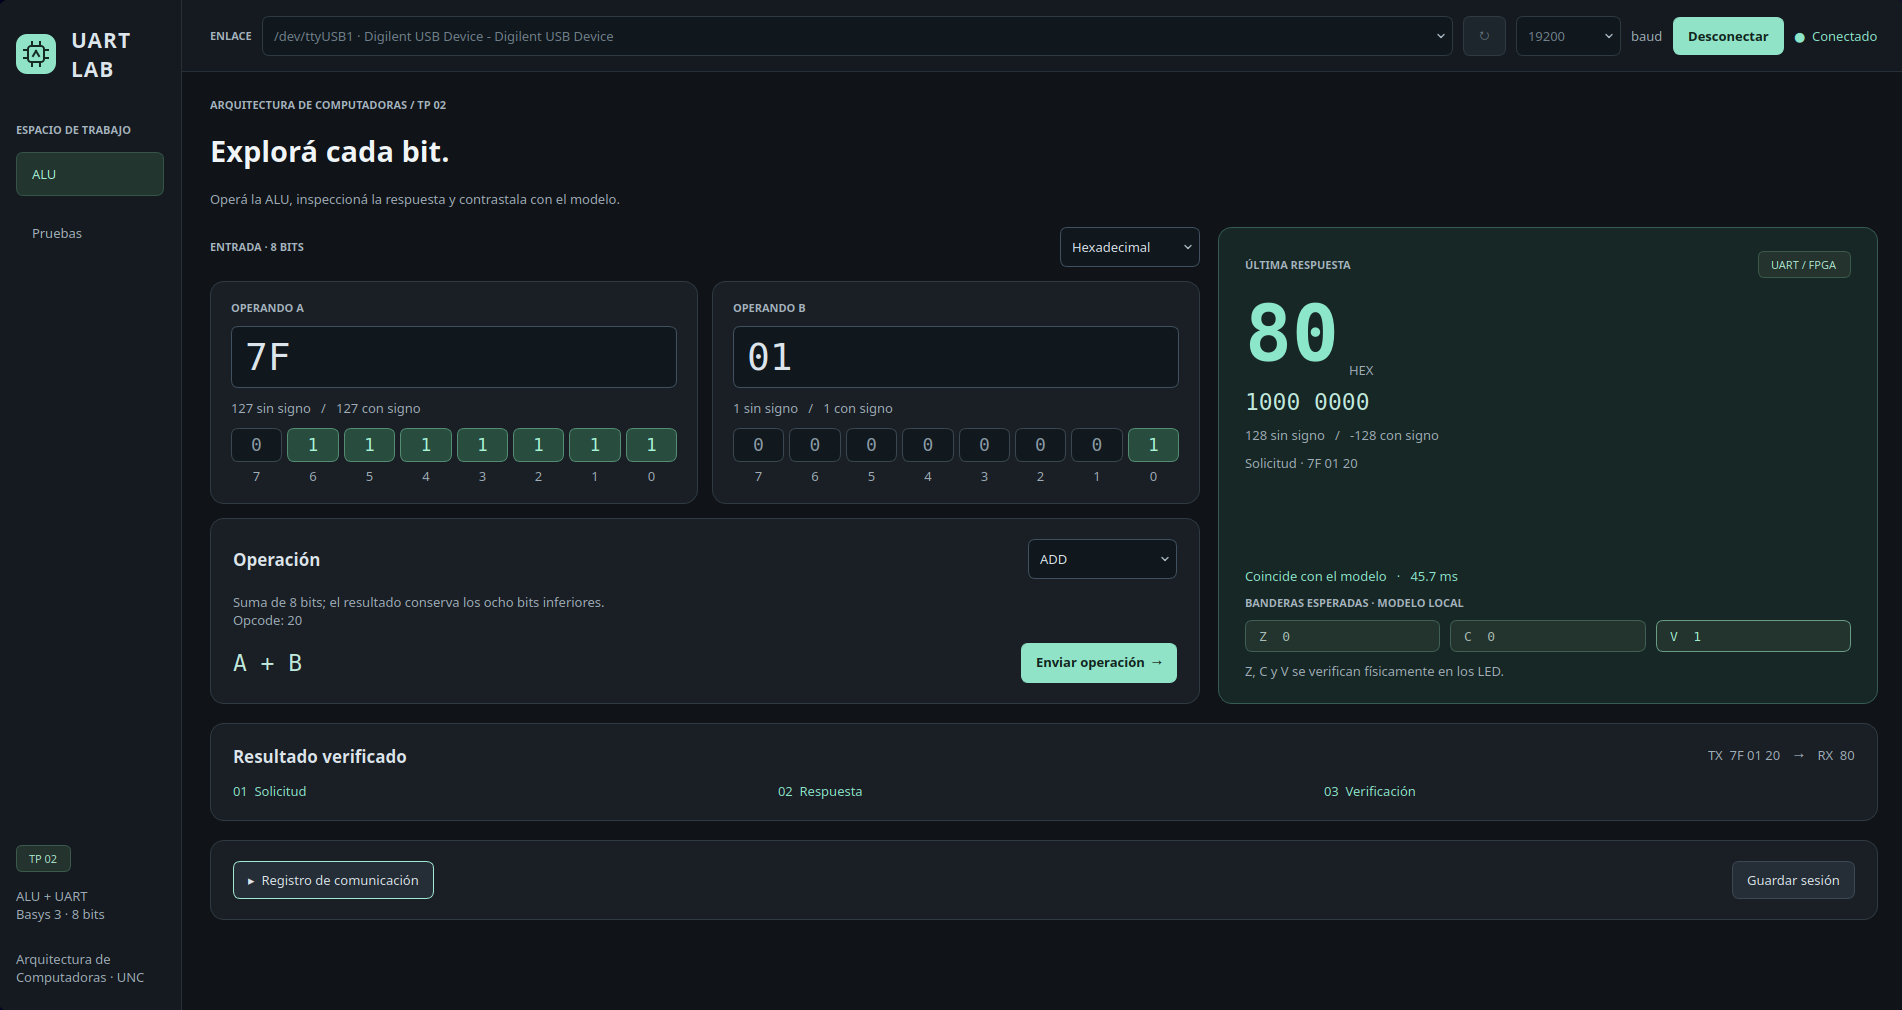
\includegraphics[width=\linewidth]{img/uart_gui_add_7f_01.png}
	\end{minipage}\hfill
	\begin{minipage}[c]{0.38\textwidth}
		\centering
		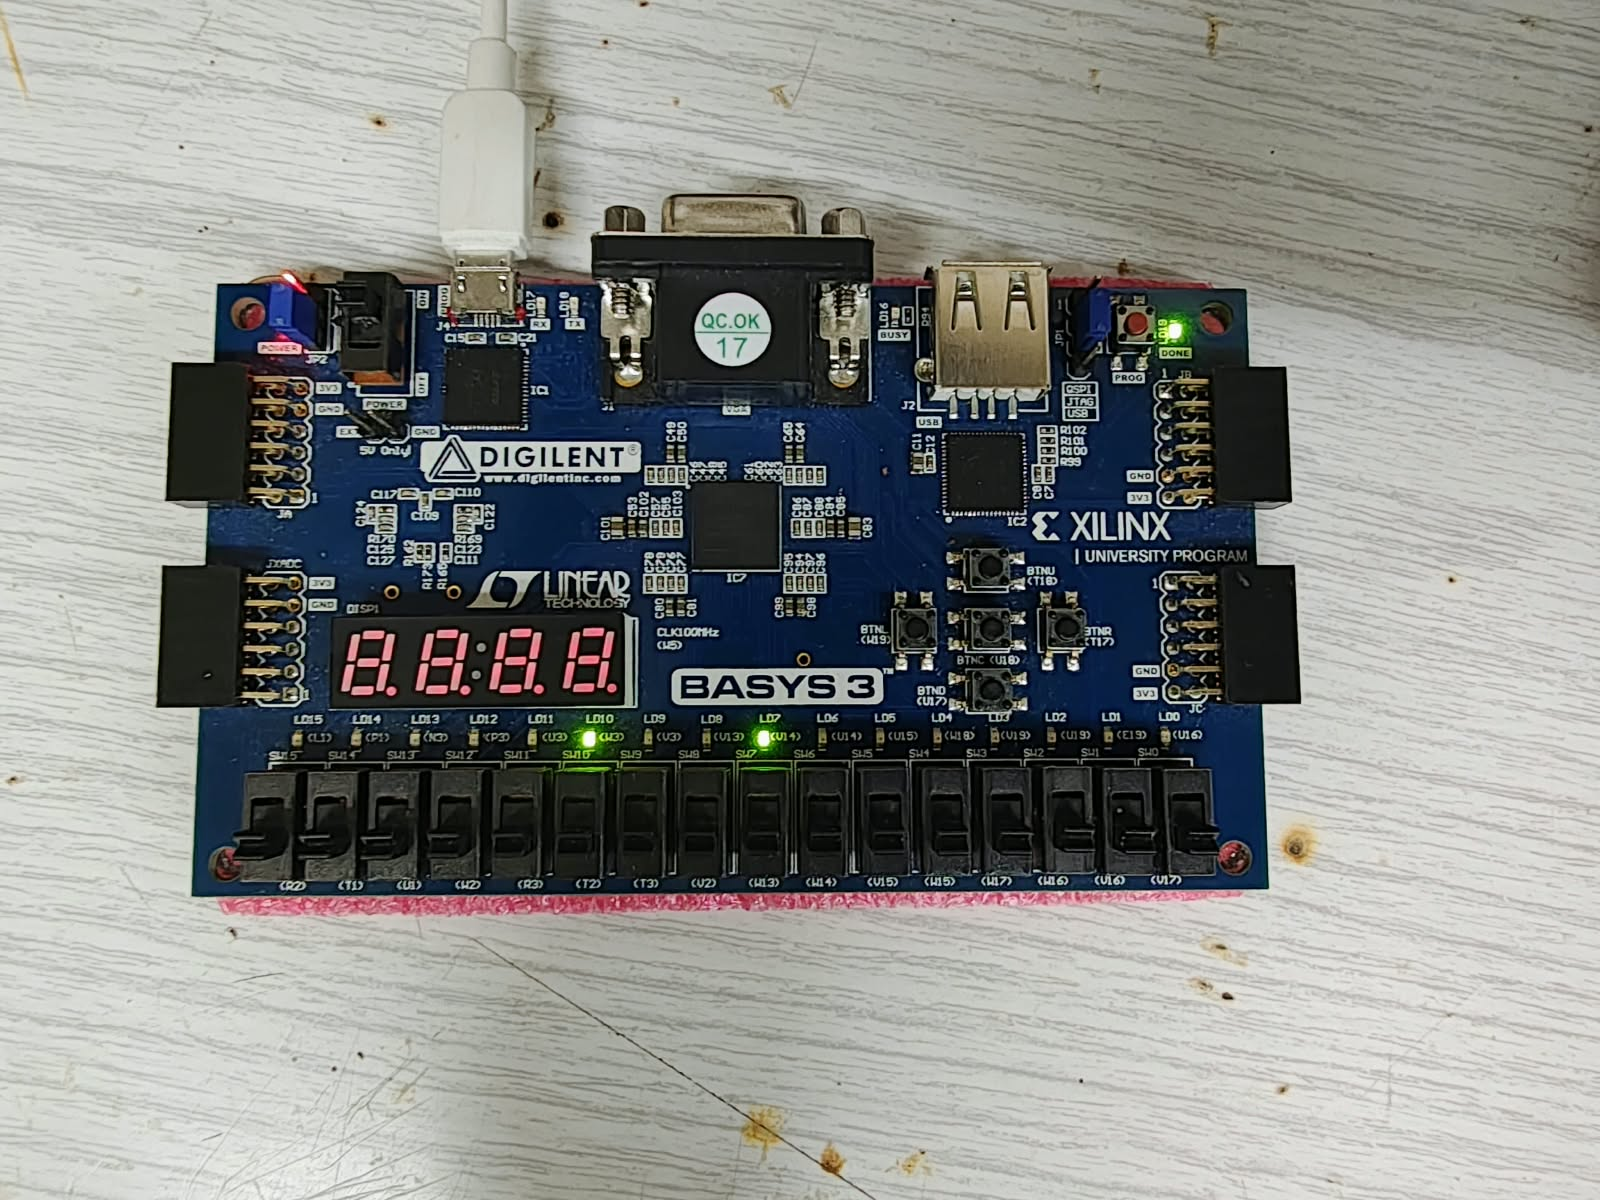
\includegraphics[width=\linewidth]{img/basys3_uart_overflow.jpg}
	\end{minipage}
	\caption{Suma \texttt{7F + 01}: respuesta \texttt{80} en la GUI y
	overflow activo en la placa.}%
	\label{fig:validacion-overflow}
\end{figure}

\section{Resultados y criterio de aceptación}

Antes de cada ensayo se fijó el resultado esperado. Se consideró aprobada una
suite cuando todas las respuestas coincidieron con el modelo, y una prueba
visual cuando el resultado UART y el patrón de LED representaron la misma
operación. La tabla~\ref{tab:validacion-fisica} resume las observaciones.

\begin{table}[H]
	\centering
	\small
	\begin{tabularx}{0.98\textwidth}{L{2.9cm}Y L{3.7cm}C{1.6cm}}
		\toprule
		\textbf{Prueba} & \textbf{Criterio} &
		\textbf{Resultado observado} & \textbf{Estado} \\
		\midrule
		Programación & Dispositivo programado y \texttt{DONE} activo. &
		\texttt{xc7a35t\_0} en estado \textit{Programmed}. & Aprobada \\
		Conexión UART & Enlace 8N1 establecido a \num{19200} baud. &
		\texttt{/dev/ttyUSB1}; GUI en estado \textit{Conectado}. & Aprobada \\
		Suite dirigida & 13 operaciones sin diferencias. &
		13 correctas; 0 diferentes. & Aprobada \\
		Suite aleatoria & 800 operaciones sin diferencias. &
		800 correctas; 0 diferentes. & Aprobada \\
		ADD \texttt{FF+01} & UART \texttt{00}; LED = \texttt{0x300}. &
		Respuesta \texttt{00}; LD8 y LD9 encendidos. & Aprobada \\
		ADD \texttt{7F+01} & UART \texttt{80}; LED = \texttt{0x480}. &
		Respuesta \texttt{80}; LD7 y LD10 encendidos. & Aprobada \\
		\bottomrule
	\end{tabularx}
	\caption{Resultados de la validación física.}%
	\label{tab:validacion-fisica}
\end{table}

La GUI transmite solicitudes completas de tres bytes y no ofrece una acción
para generar deliberadamente una trama parcial. En consecuencia, la
recuperación por timeout no formó parte de esta campaña física. Ese mecanismo
se verificó de manera específica en los bancos de prueba del controlador y del
sistema integrado, donde sí fue posible controlar con precisión el intervalo
entre bytes. Esta separación evita presentar como observación sobre la placa
una condición que no fue producida durante el ensayo.

\section{Interpretación}

Las pruebas físicas abarcaron la cadena completa: selección del puerto,
transmisión desde la GUI, recepción UART, almacenamiento temporal,
interpretación de la terna, ejecución de la ALU, transmisión de la respuesta y
retención del resultado en los LED. La suite dirigida ejercitó situaciones de
frontera y la suite pseudoaleatoria amplió el conjunto con 800 operaciones
reproducibles. En total se completaron 815 transacciones físicas sin diferencias
respecto del modelo de referencia.

Las comprobaciones visuales agregaron evidencia que el byte UART no puede
aportar por sí solo: demostraron que el resultado retenido y las banderas Z, C
y V correspondieron a la misma operación informada a la computadora. En
conjunto, los resultados de la tabla~\ref{tab:validacion-fisica} permiten dar
por aceptado el funcionamiento extremo a extremo del sistema en la Basys 3.


\chapter{Conclusiones}
\begingroup
\setlength{\parskip}{0.30em}
Como se planteó en la sección~\ref{chap:introduccion}, este trabajo
cambió el centro del problema respecto del TP1. La ALU siguió siendo
el bloque encargado de realizar las operaciones, pero ya no recibió
los operandos de forma directa mediante los switches de la placa. En
este caso fue necesario construir una UART capaz de recibirlos y
transmitir el resultado de manera serial. Esto hizo que el diseño
dejara de depender solamente de los valores presentes en las entradas
y pasara a depender también del orden en que llegan y del momento en
que se producen los distintos eventos.

Como se vio en la sección~\ref{chap:nucleo-uart}, dedicada al núcleo
UART, las máquinas de estado finitas permitieron organizar este
comportamiento temporal de una forma clara. En la recepción, la FSM
espera el inicio de una trama, valida el bit de start, reconstruye el
byte a medida que llegan sus bits y comprueba finalmente el bit de
stop. En la transmisión ocurre el recorrido inverso: a partir de un
byte se generan, en el orden y durante el tiempo correspondiente, el
start, los ocho bits de datos y el stop. El generador de ticks y el
sobremuestreo proporcionan la referencia temporal para que ambas
máquinas puedan avanzar por esas etapas y trabajar con una señal que
no comparte el reloj de la FPGA.

La tercera máquina de estados, presentada en la
sección~\ref{sec:controlador-transacciones}, unió la comunicación con
la ALU. Sus estados representan las distintas etapas de una
operación: esperar los dos operandos, recibir el código de operación,
registrar el resultado y entregarlo para su transmisión. Esta
separación permitió expresar de manera directa qué información debía
conservarse en cada momento y evitó que la interpretación del
protocolo quedara mezclada con la recepción bit a bit. De esta forma,
las tres FSM resolvieron partes diferentes del mismo intercambio y,
al trabajar en conjunto, hicieron posible completar el recorrido
desde la entrada RX hasta la respuesta por TX.

La implementación también permitió llevar a la práctica los criterios
de diseño de máquinas de estado estudiados en la consigna. La
distinción entre el estado actual, el próximo estado y las salidas
hizo más sencillo seguir las transiciones tanto en el código como en
las formas de onda. A su vez, la codificación one-hot resultó
adecuada para la FPGA y facilitó reconocer cada estado durante la
verificación. Las ramas de recuperación y los estados de espera
fueron igualmente importantes, porque una UART no solo debe procesar
tramas válidas, sino también volver a una situación conocida frente a
una entrada incompleta, un error de trama o un estado no contemplado.

Además de lo requerido para implementar la UART, se incorporaron
recursos que mejoraron la robustez del sistema. Los sincronizadores
acondicionaron las señales externas, mientras que las colas FIFO
permitieron desacoplar por un breve intervalo la comunicación y el
procesamiento. El timeout y el manejo de esperas completaron esa idea
al impedir que una operación incompleta o una salida momentáneamente
ocupada dejara al controlador en una situación indefinida. Si bien
estos elementos no constituyen el objetivo principal del trabajo,
ayudaron a integrar las máquinas de estado en un sistema más
confiable y cercano a una aplicación real.

Finalmente, las pruebas presentadas en las
secciones~\ref{chap:verificacion} y~\ref{chap:validacion} permitieron
observar las transiciones de cada FSM por separado y comprobar
después su funcionamiento conjunto. Las simulaciones mostraron la
recepción y transmisión de tramas, la secuencia seguida por el
controlador y la recuperación ante errores, mientras que los ensayos
sobre la Basys 3 confirmaron que una solicitud enviada desde la
computadora podía atravesar todo el sistema y producir la respuesta
esperada. En conjunto, el trabajo permitió comprender que una UART no
se reduce a desplazar bits: requiere modelar una secuencia completa
de acciones, conservar el progreso entre ciclos y definir con
precisión cómo avanzar o recuperarse. En ese sentido, las máquinas de
estado fueron la herramienta central que permitió transformar el
protocolo UART en un circuito digital ordenado, verificable y sintetizable.

\endgroup

\chapter*{Referencias}
\addcontentsline{toc}{chapter}{Referencias}
\begin{itemize}
    \raggedright
  \item Cátedra de Arquitectura de Computadoras, \textit{Máquinas de Estado
    Finitas --- TP: UART}, filminas y consigna provistas en
    \texttt{5 - Maquinas de Estado Finitas.pdf}.
  \item Arnaudo, F. A. y Perotti, F. J., \textit{Unidad
    Aritmético-Lógica}, Trabajo Práctico Nº 1, fuentes SystemVerilog,
    testbenches e informe incluidos en este repositorio.
  \item Pong P. Chu, \textit{FPGA Prototyping by Verilog Examples:
    Xilinx Spartan-3 Version}, capítulo sobre comunicación serie UART,
    Wiley, 2008.
  \item Digilent, \textit{Basys 3 Reference Manual}. Disponible en
    \url{https://digilent.com/reference/_media/reference/programmable-logic/basys-3/basys3_rm.pdf}.
  \item Digilent, \textit{Basys 3 Master XDC}. Disponible en
    \url{https://github.com/Digilent/digilent-xdc}.
  \item AMD, \textit{Vivado Design Suite User Guide: Programming and
    Debugging}, UG908, procedimiento de conexión y programación mediante
    Hardware Manager. Disponible en
    \url{https://docs.amd.com/r/2025.1-English/ug908-vivado-programming-debugging/Opening-Hardware-Target-Connections}.
  \item AMD, \textit{Vivado Design Suite User Guide: Using Constraints},
    UG903, documentación de restricciones y análisis temporal.
  \item IEEE, \textit{Standard for SystemVerilog---Unified Hardware Design,
    Specification, and Verification Language}, IEEE 1800.
\end{itemize}


\end{document}
